\documentclass[twoside, 12pt, openright, final]{memoir}

%%%%%%%%%%%%%%%%%%
% For margins etc, our text area has a height of 167.5mm and a width of 130mm
%%%%%%%%%%%%%%%%%%
\setstocksize{240mm}{170mm}
\settrimmedsize{\stockheight}{\stockwidth}{*}
\settrims{0mm}{0mm}
\setmarginnotes{0mm}{0mm}{0mm}
\setlrmarginsandblock{20mm}{20mm}{*}
\setulmarginsandblock{42.5mm}{30mm}{*}
\setheadfoot{10mm}{15mm}
\setheaderspaces{*}{7.5mm}{*}
\checkandfixthelayout

%%%%%%%%%%%%%%%%%%%%%%%%%%%%%%%%%%%%%
%For font
%%%%%%%%%%%%%%%%%%%%%%%%%%%%%%%%%%%%%
\usepackage{lmodern}
\usepackage[T1]{fontenc}
\renewcommand{\familydefault}{\sfdefault} 

%%%%%%%%%%%%%%%%%%%%%%%%%%%%%%%%%%%%%%
%For pagestyle, chapterstyle, bibliography
%%%%%%%%%%%%%%%%%%%%%%%%%%%%%%%%%%%%%%
\pagestyle{ruled}
\chapterstyle{bianchi}

%%%%%%%%%%%%%%%%%%%%%%%%%%%%%%%%%%%%%%
%For creating thumb indices
%%%%%%%%%%%%%%%%%%%%%%%%%%%%%%%%%%%%%%
%\usepackage{thumby}
%\thumbySides{two}
%\thumbyTotalChapters{2}

%%%%%%%%%%%%%%%%%%%%%%%%%%%%%%%%%%%%%%%
% Other packages
%%%%%%%%%%%%%%%%%%%%%%%%%%%%%%%%%%%%%%%
%For equations, the tbtags option puts line numbers at the last line of a multiline equation
\usepackage[final]{pdfpages}
\usepackage[tbtags]{amsmath}
\DeclareMathOperator{\argmax}{arg\,max}
\DeclareMathOperator{\argmin}{arg\,min}
%For \url
\usepackage{hyperref}
%For colored text
\usepackage{xcolor}
\definecolor{GREEN}{RGB}{51, 160, 44}

%For subsection numbering
\setsecnumdepth{subsection}

%For \includegraphics
\usepackage{graphicx}
%For small caption sizes of figures and tables
\usepackage{caption}
\captionsetup[figure]{font=small}
\captionsetup[table]{font=small}
%For Tikz figure used in the biometrics paper
\usepackage{tikz}
\usetikzlibrary{shapes.geometric, arrows, positioning}

\tikzstyle{startstop_big} = [rectangle, rounded corners, minimum width=3cm, minimum height=1cm,text centered, draw=black,text width = 8.5cm, fill=red!30]
\tikzstyle{startstop} = [rectangle, rounded corners, minimum width=3cm, minimum height=1cm,text centered, draw=black,text width = 5cm, fill=red!30]
\tikzstyle{io} = [trapezium, trapezium left angle=70, trapezium right angle=110, minimum width=2cm, minimum height=1cm, text centered, draw=black, fill=blue!30]
\tikzstyle{process} = [rectangle, minimum width=3cm, minimum height=1cm, text centered, text width = 3cm, draw=black, fill=orange!30]
\tikzstyle{process_wide_3pt5cm} = [rectangle, minimum width=3cm, minimum height=1cm, text centered, text width = 3.5cm, draw=black, fill=orange!30]
\tikzstyle{process_wide_4cm} = [rectangle, minimum width=3cm, minimum height=1cm, text centered, text width = 4cm, draw=black, fill=orange!30]
\tikzstyle{process_wide_4pt5cm} = [rectangle, minimum width=3cm, minimum height=1cm, text width = 4.5cm, draw=black, fill=orange!30]
\tikzstyle{process_wide_5cm} = [rectangle, minimum width=3cm, minimum height=1cm, text width = 5cm, draw=black, fill=orange!30]
\tikzstyle{decision} = [diamond, minimum width=1cm, minimum height=1cm,text centered,text width = 2.25cm, draw=black, fill=green!30]
\tikzstyle{arrow} = [thick,->,>=stealth]


%%%%%%%%%%%%%%%%%%
%For bibliography
%%%%%%%%%%%%%%%%%%%
\usepackage[sectionbib]{natbib}
\usepackage{chapterbib}
\renewcommand{\bibname}{References}

%%%%%%%%%%%%%%%%%%%%%%%%%%%%%%%%%%
%Document contents here onwards
%%%%%%%%%%%%%%%%%%%%%%%%%%%%%%%%%%
\begin{document}
%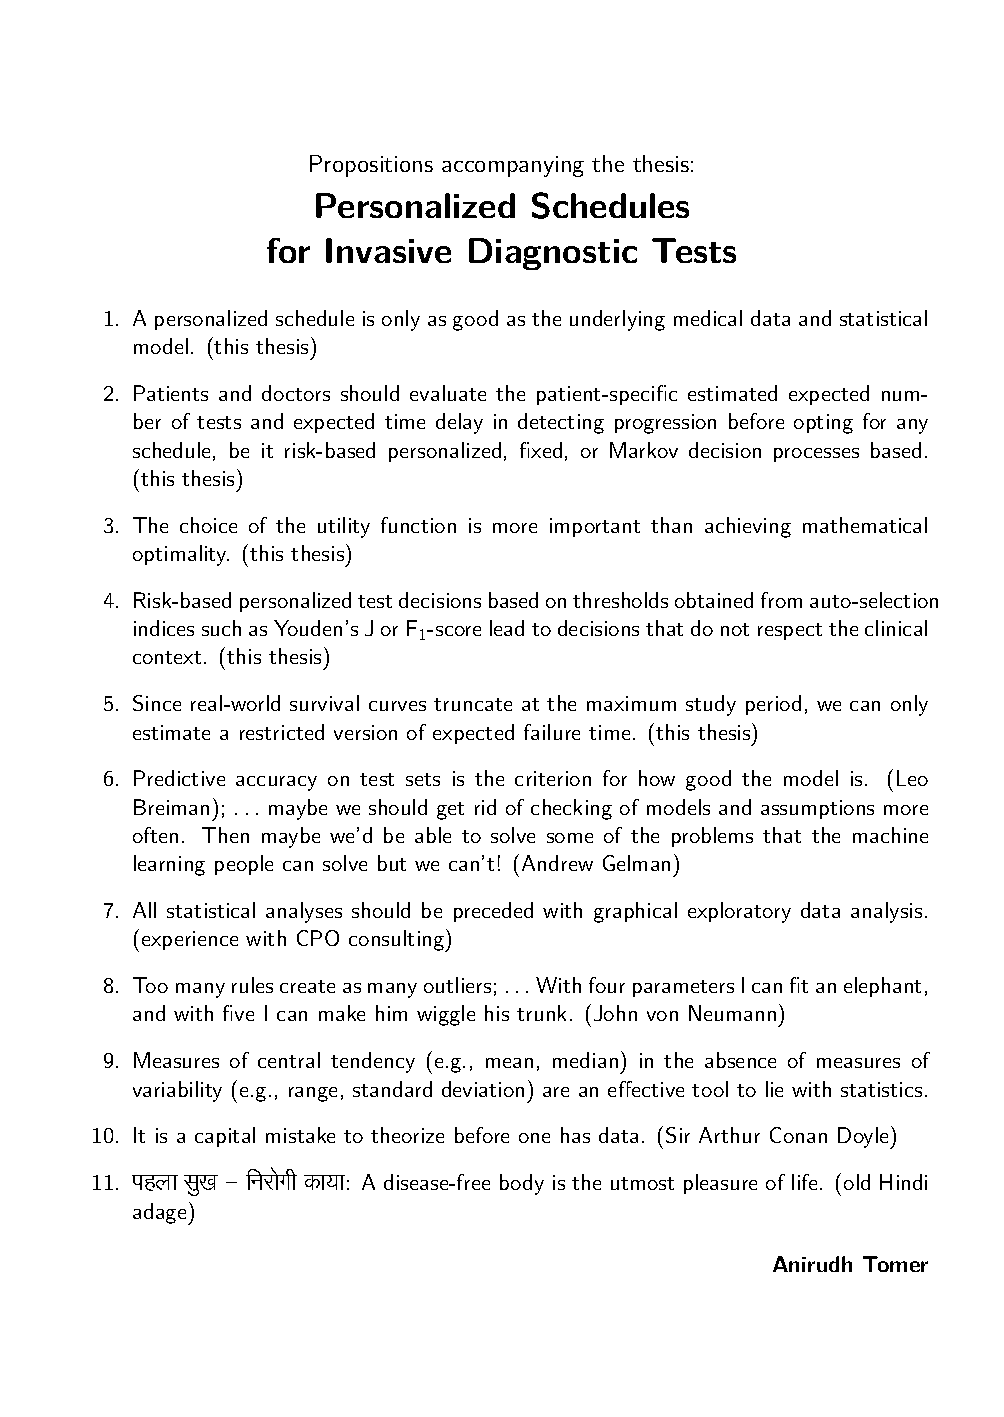
\includepdf{propositions.pdf}
\frontmatter

%Real title page
\begin{titlingpage} 
%\title{\emph{Title of your thesis Title of your thesis Title of your thesis Title of your thesis}}
%\author{Author of the thesis}
%\date{\today}

%\maketitle
\raggedleft
\vspace*{\baselineskip}
{\Huge\itshape Personalized Schedules for\\ Invasive Diagnostic Tests}\\[\baselineskip]
{\large\itshape With Applications in Surveillance \\of Chronic Non-Communicable Diseases}\\[0.2\textheight]
{\Large Anirudh Tomer}\par
\vfill
{\Large Rotterdam, \today}
\vspace*{\baselineskip}
\end{titlingpage}

\includepdf[pages=-]{title_page.pdf}
%Dedication page
\begin{titlingpage} 
\thispagestyle{plain}
\par\vspace*{.35\textheight}{\centering Dedicated to my parents,\\ medical science, and patients worldwide\par}
\end{titlingpage}

\tableofcontents
\mainmatter
\chapter[General Introduction][General Introduction]{General Introduction}
\label{c1}

\cleardoublepage

\section{Chronic Disease Surveillance}
\label{c1:sec:invasive_tests}
Non-communicable diseases (NCDs) such as cancer, diabetes, cardiovascular, and respiratory diseases are a 21st-century global pandemic. They affect men and women equally and cause 60\% to 70\% of all human deaths worldwide~\citep{world2014global, bennett2018ncd}. Often NCDs are chronic. Hence, in many \emph{low-risk} NCD diagnoses (e.g., localized prostate cancer, low-risk dysplasia), immediate serious treatments like surgery, radiotherapy, etc., can induce side-effects and reduce a patient's overall quality of life. A common alternative to immediate treatment is delaying it until the disease has \emph{progressed}, a curable non-terminal disease stage. In this regard, monitoring patients for progression, with curative intent, is called \emph{surveillance}. 

The goal of surveillance is to timely detect progression, upon which patients are typically removed and treated. However, the transition of a patient's \emph{disease state} from low-risk to progressed disease is not directly observable. Instead, auxiliary modalities such as biomarkers, physical examinations, medical imaging, biopsies, etc., are used to determine the disease state. Among these, the gold standard \emph{tests} for confirming progression are typically \emph{invasive} (e.g., biopsies). For timely observing the occurrence of progression, invasive tests are conducted repeatedly in surveillance. For example, biopsies are the benchmark test for verifying progression in surveillance of localized prostate cancer~\citep{bokhorst2015compliance}. Similarly, endoscopies are utilized in Barrett's esophagus~\citep{choi2012screening} and colonoscopies in colorectal cancer~\citep{krist2007timing} surveillance. Repeat bronchoscopies, and core biopsies are also employed to detect allograft deterioration in lung~\citep{mcwilliams2008surveillance} and kidney transplant~\citep{henderson2011surveillance} patients, respectively.

\subsection{Invasive Test: Burden versus Benefit}
Currently, repeated invasive tests are a necessary \emph{burden} for patients. They are indispensable for confirming progression, but they are also difficult to perform, may cause pain, and can lead to severe complications~\citep{loeb2013systematic,krist2007timing}. Consequently, invasive tests are usually planned with a considerable time gap between them. For example, in prostate cancer surveillance, it is recommended to maintain a time difference of one year between consecutive biopsies. However, a time gap between tests also leads to a \emph{time delay} in detecting progression (Figure~\ref{c1:fig:1}). When tests are conducted periodically, this delay can be reduced by scheduling tests frequently. The argument for lowering delay is that detecting progression earlier may provide a larger window of opportunity for curative treatment. Also, timely treatment may also have an impact on the patient's (quality-adjusted) life-years remaining. Hence, a balance between the number and frequency of tests (burden) and time delay in detecting progression (shorter is beneficial) is of crucial importance for patients.

\begin{figure}[tbp]
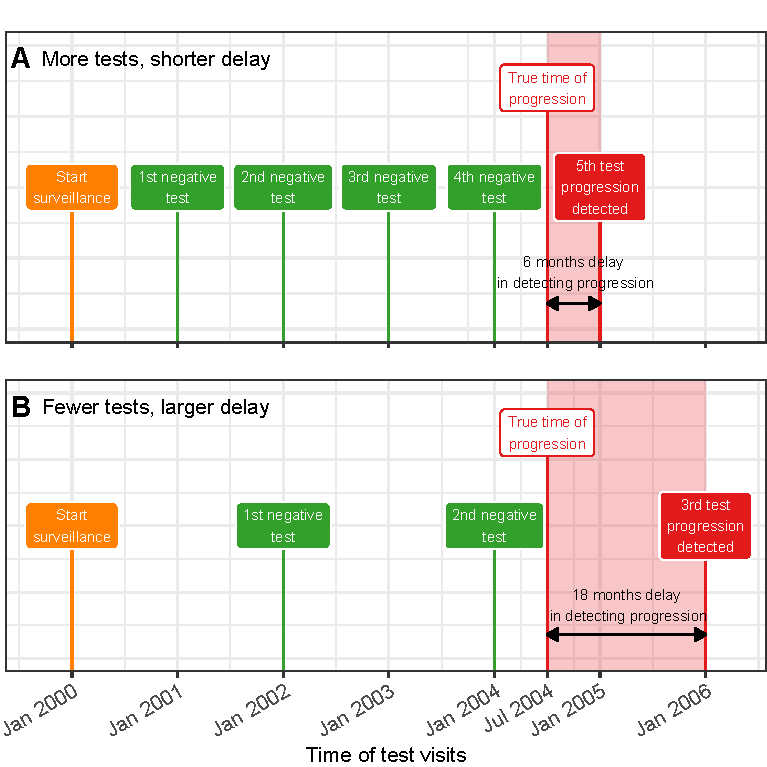
\includegraphics{contents/c1/images/c1_fig1.pdf}
\caption{\textbf{Trade-off between the test frequency and the time delay in detecting disease \emph{progression}:} The true time of disease progression for the patient in this figure is July 2008. More frequent tests in \textbf{Panel~A}, lead to a shorter time delay in detecting progression, than fewer tests in \textbf{Panel~B}. Due to the periodical nature of tests, the time of progression is always observed as an interval. For example, between Jan~2004--Jan~2005 in \textbf{Panel~A} and between Jan~2004--Jan~2006 in \textbf{Panel~B}.}
\label{c1:fig:1}
\end{figure}

\subsection{Schedules for Invasive Tests}
\label{c1:subsec:scheduling_methodologies}
The frequency of invasive tests varies across diseases and cohorts. However, within a cohort, usually a constant frequency or \emph{fixed schedule} (e.g., every six months) is employed for all patients~\citep{henderson2011surveillance,bokhorst2015compliance,krist2007timing}. The primary drawback of a fixed schedule is its \emph{one-size-fits-all} assumption. Specifically, high-frequency tests promise shorter delays in detecting progression at the cost of imposing an extra burden on patients who progress slowly and/or patients who never experience progression (e.g., due to comorbidities). The vice versa holds for infrequent tests. Schedules with a skewed burden benefit ratio are also prone to patient non-compliance~\citep{bokhorst2015compliance,LeClercq2015325}. Reduced compliance for invasive tests may lead to the original problem of delayed detection of disease progression, and reduce the effectiveness of surveillance. 

Several improvements have been proposed over one-size-fits-all fixed schedules. The underlying methodology of these advances can be broadly divided into three categories. Namely, sub-group specific fixed schedules, schedules cost-optimized using Markov decision processes, and schedules optimizing a specific utility function of the clinical parameters of interest. Two commonly used terms across these three methodologies are \emph{personalized/individualized/tailored} schedules, and \emph{optimal} schedules. Loosely, personalization means a unique schedule for each patient in a study population. Optimal refers to mathematical optimization of certain schedule-specific criteria to automatically derive a schedule.

\paragraph{Sub-group specific fixed schedules}
These schedules are typically prescribed based on observed patient data such as biomarkers, physical examinations, medical imaging, or previous test results. For example, in Barrett's esophagus patients observing low-risk dysplasia on a repeat endoscopy are prescribed future endoscopies every six to twelve months, rather than the standard once every three to five years~\citep{choi2012screening}. Sub-groups are also formed based on multiple results. For example, in the world's largest prostate cancer surveillance PRIAS, the time of biopsies is decided using observed \emph{prostate-specific antigen (PSA)} value, the average rate of change of PSA, the size and shape of the tumor, and previous biopsy results (Figure~\ref{c1:fig:c1_prias_biopsy_protocol}). There are two main shortcomings of such heuristic schedules. First, they often create sub-groups based on observed data without accounting for ascertainment biases and measurement error. Second, as illustrated in Figure~\ref{c1:fig:c1_prias_biopsy_protocol}, instead of utilizing complete observed data, they typically use only the latest observed value, that too after categorizing continuous ones.

\begin{figure}[tbp]
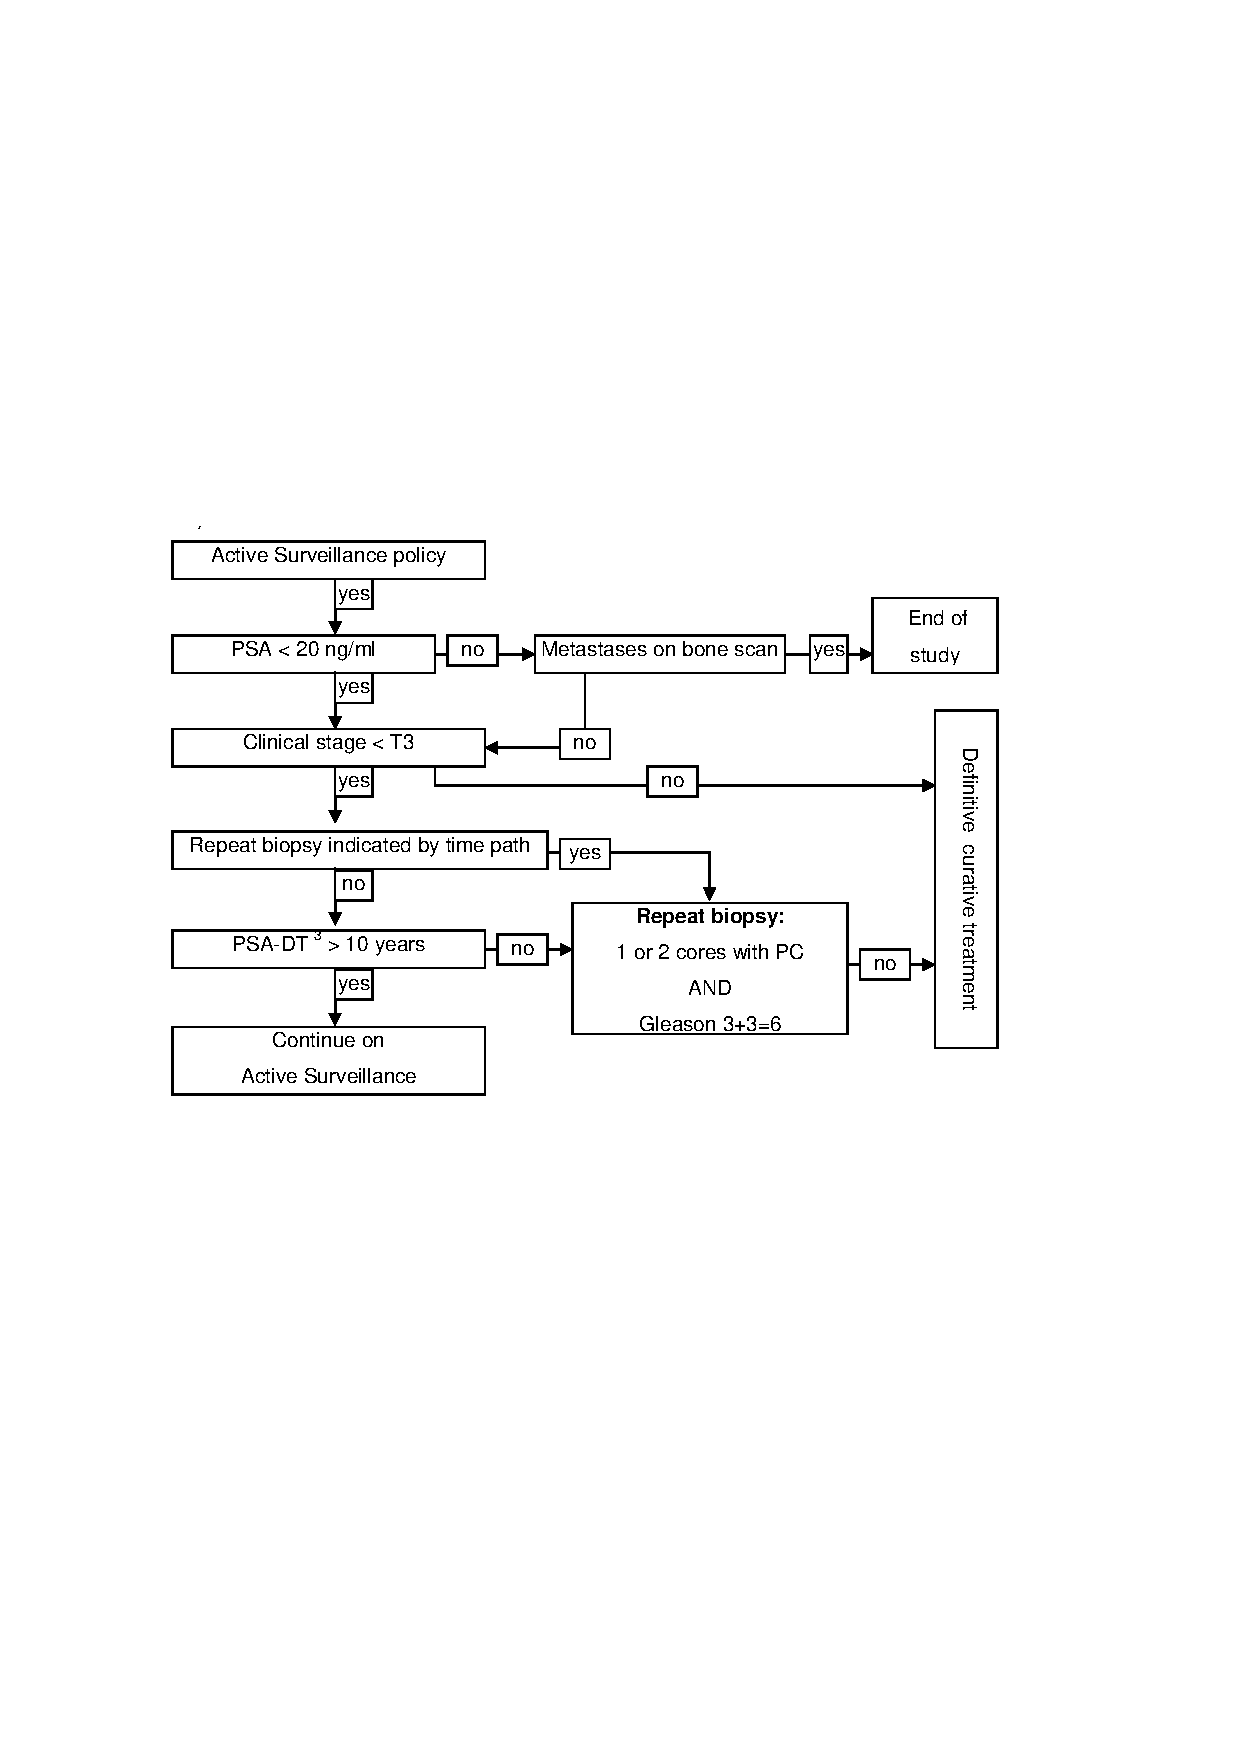
\includegraphics{contents/c1/images/c1_prias_biopsy_protocol.pdf}
\caption{\textbf{Treatment and biopsy protocol} of the world's largest localized prostate cancer surveillance program PRIAS. Source:~\url{https://www.prias-project.org}}
\label{c1:fig:c1_prias_biopsy_protocol}
\end{figure}

\paragraph{Partially observable Markov decision processes} or POMDPs have been utilized in numerous optimal screening and surveillance test schedules for chronic diseases~\citep{steimle2017markov,denton2018optimization}, and especially for nearly all types of cancers~\citep{alagoz2010operations}. A notable advantage of POMDPs is that they find an optimal schedule from all schedules possible over a set of follow-up visits. The criterion of optimality in POMDPs is the weighted cumulative reward. A reward is a number that is chosen manually for four possible outcomes (true-positive, false-positive, true-negative, and false-negative) of a binary test/no test decision in a schedule. The weighted cumulative reward of a schedule is the weighted sum of all rewards possible with all sequential test decisions in a schedule. The weights are probabilities from a joint probability distribution of the disease state of the patient and the auxiliary outcomes (e.g., biomarkers) that manifest this state. This joint distribution is allowed to change over time.

In general, POMDP algorithms suffer from the curse of dimensionality if continuous longitudinal outcomes or continuous time-space is used~\citep{sunberg2018online}. However, a more substantial drawback of POMDPs is their very flexible specification. Specifically, in a simple POMDP with binary test/no test decisions, and binary disease state (low-risk, progressed), it can be shown that there exist infinite possible rewards result in the same optimal schedule (Chapter~\ref{c4:appendix:pomdp}). Typically POMDP rewards are chosen based on survey results~\citep{denton2018optimization} and translated as quality-adjusted life-years saved. However, with infinite optimal reward sets, any reward set can be cherry-picked, including those that correspond to (improbable) thousands of quality-adjusted life-years saved. Last, to our knowledge, POMDPs are not currently personalized. Since they exploit population-level joint distributions of disease state (e.g., Kaplan-Meier curve) and auxiliary outcomes, the resulting schedules are not personalized.

\paragraph{Schedules optimized for clinical parameters of interest} An option to the POMDP framework is optimizing a utility function of the clinical parameters of interest directly~\citep{bebu2018optimal,parmigiani1996optimal}. Examples of clinical parameters are, namely, the financial cost for treating progression, reduction in lifespan due to delayed detection of progression, cost of invasive tests, reduction in quality of life due to invasive tests. Others have proposed optimizing test decision rules for the corresponding sensitivity and specificities in detecting progression~\citep{wang2019learning}. Alternatively, one may optimize information-theoretic measures such as Wasserstein distance~\citep{hanin2001optimal} or Kullback-Leibler divergence~\citep{rizopoulos2016personalized} between the disease state probability distribution at the beginning of surveillance and at a future time point. 

In all of these approaches, the expected utility is calculated using the probability distribution of the disease state of the patient. It is standard to use a time-varying disease state distribution. Although, this distribution can be either discrete (e.g., a Markov model with low-risk, medium-risk, progressed disease states) or continuous (e.g., Cox model).

\subsection{Goal: Developing Personalized Schedules}
\label{c1:subsec:goal}
The overall aim of this work was to develop personalized schedules that better balance the overall burden and benefit of repeated invasive tests in surveillance than one-size-fits-all fixed schedules. The subgoals and specific research questions that we intend to answer in this work are as follows.
\begin{itemize}
  \item To find a suitable statistical modeling framework to process observed patient data. 
  \item Evaluating the efficacy of different utility functions while planning tests by optimizing clinical parameters of interest (e.g., time delay in detecting progression).
  \item Evaluating the pros and cons of the widely used POMDP framework for scheduling tests.
  \item How to schedule invasive tests based on a patient's risk of progression?
  \item On which criteria should patients chose a personalized schedule over a fixed schedule and vice versa?
  \item Which factors (e.g., cohort, type of disease) affect the performance of a personalized schedule?
  \item Can the same test scheduling framework be used across different cohorts and diseases?
\end{itemize}
To answer our research questions and to develop personalized schedules, the process we followed consisted of four steps. First, processing the observed data of the patient. For example, directly using data via flowcharts (Figure~\ref{c1:fig:c1_prias_biopsy_protocol}), using summary statistics, and statistical modeling of observed data, etc. Second, choosing the reward/utility/loss function and the corresponding clinical parameters. Third, defining criteria and methodology for comparing proposed personalized schedules with currently practiced schedules. Fourth, implementing personalized schedules in a computer application for practitioners. 

\paragraph{Processing observed data} In surveillance, observed data consists of baseline patient characteristics, longitudinally measured outcomes, and previous invasive test results. Since all of these manifest the underlying disease state of the patient, they are usually correlated as well. To accommodate outcomes of various types, we utilized the framework of joint models for time-to-event and longitudinal data~\citep{rizopoulos2012joint, tsiatis2004joint}. The motivation of this choice was that joint models combine observed data into a patient-specific cumulative-risk of progression over the entire follow-up period. This risk profile manifests the underlying latent disease state of the patient.

\paragraph{Choosing of reward/utility/loss function and clinical parameters of interest} Once a risk profile for progression is available, the next step is to utilize it for optimizing clinical parameters of interest. Examples of these parameters are the time of disease progression, time delay in detecting disease progression given a schedule (Figure~\ref{c1:fig:1}), number and timing of tests in a schedule, cumulative-risk of disease progression, sensitivity/specificity of an invasive test and their derivatives such as Youden index and F1score~\citep{lopez2014optimalcutpoints}. We optimized these parameters via both standard utility functions such as squared loss, absolute loss, multilinear loss~\citep{robertBayesianChoice}, and custom utility functions that are a linear sum of multiple clinical parameters of interest.

\paragraph{Comparing personalized versus fixed schedules} There are no single perfect criteria to compare schedules. Some important ones, though, are how many patient deaths and/or progression to an advanced disease state (e.g., metastasis) are saved. Reliable data on such metrics are difficult to obtain in low-grade diseases. This is because, in such diseases, the prevalence of death from disease can be quite low (e.g., almost zero in low-grade prostate cancer active surveillance). Hence in this work, we used two other criteria for comparing the performance of proposed personalized schedules with existing fixed schedules; Specifically, the number and timing of invasive tests (burden of tests) and time delay in the detecting progression (shorter is beneficial). Our choice of these criteria is motivated by two reasons. First, we argue that time delay in detection of progression is an easily-quantifiable surrogate for important clinical aspects such as the window of opportunity for curative treatment, risk of adverse downstream outcomes, quality-adjusted remaining lifetime, and additional complications in treating a delayed progression. Similarly, the number and timing of tests manifest financial costs of tests, risk of side-effects, and reduction in quality of life, etc. Second, both the number of tests and time delay in detecting progression are easy to understand for both patients/doctors and can better facilitate \emph{shared decision making} of test schedules.

\paragraph{Computer application implementing personalized schedules} While there is no lack of existing methodologies for making invasive test schedules, presenting them in a user-friendly computer/web/phone application may increase their awareness and/or adoption. In this regard, we implemented personalized schedules in a web-application for real patients of the seven largest prostate cancer active surveillance programs. Also, we provide our scheduling methodology as a generic R application programming interface for surveillance of other diseases.
\section{A Joint Model for Time-to-progression and Longitudinal Data}
\label{c1:sec:jm}
The first step in developing personalized schedules is processing a patient's surveillance data. This data includes baseline patient features, longitudinally measured outcomes of different types, and previous invasive test results. There are several challenges in modeling such data. First, longitudinal outcomes can be of different types (e.g., binary, continuous), are measured with error, and possibly correlated with each other. Second, usually, longitudinal measurements are not available after the patient is removed from surveillance upon observing progression. Third, patients who observe progression can have more adverse longitudinal data values. Fourth, time of progression is interval-censored (Figure~\ref{c1:fig:1}). Last, combining all this data to obtain a patient's personalized risk of progression. To overcome these challenges, we utilize the framework of joint models for time-to-event and longitudinal data~\citep{rizopoulos2012joint, tsiatis2004joint}.

\begin{figure}[tbp]
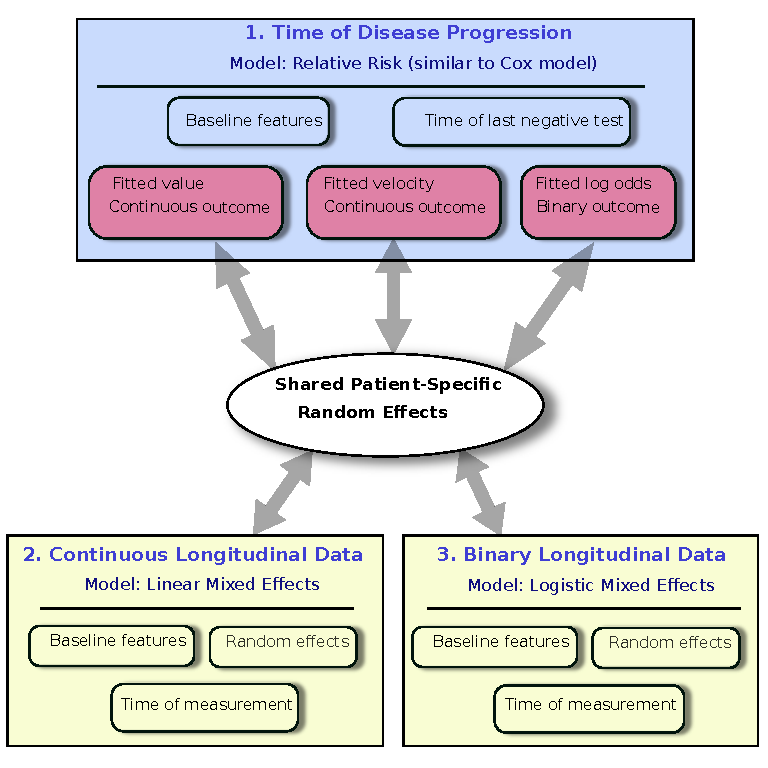
\includegraphics{contents/c1/images/c1_jm_blockdiag.pdf}
\caption{\textbf{Block diagram of a joint model for time-to-progression and longitudinal data}. Typically mixed effect sub-models are utilized for longitudinally measured data, and a relative-risk sub-model is employed for the interval-censored time of progression. The outcomes in these sub-models are conditionally independent of each other, given the common source of correlation patient-specific random-effects~\citep{laird1982random}. Different features of the longitudinal outcomes such as their fitted value, rate of change, fitted log-odds can be included in the relative-risk sub-model for predicting the risk of progression.} 
\label{c1:fig:c1_jm_blockdiag}
\end{figure}

The primary component in joint models is patient-specific random effects~\citep{laird1982random}. They represent the underlying state of disease, as well as act as the common source of correlation between different outcomes (Figure~\ref{c1:fig:c1_jm_blockdiag}) of a patient. Each outcome has a separate sub-model. Usually, mixed-effect sub-models are used for longitudinal outcomes, and a relative risk sub-model is employed for time-to-progression data. The parameters of the different sub-models are estimated jointly. Given a patient's data, the key output from the fitted joint model is a patient's personalized cumulative-risk of progression.

\subsection{Cumulative-risk of Progression}
Consider a joint model is fitted to a particular dataset. Given a new patient's accumulated data, the fitted joint model can predict his cumulative-risk of progression over his entire follow-up period starting from the time of his last negative test. This risk profile manifests the transition of a patient's disease state over time from low-risk to progressed. Hence, it can be used to guide the timing of invasive tests. In this regard, we have not only used the cumulative-risk to create personalized schedules but also for calculating a patient's expected time of progression. Although we estimate cumulative-risk using joint models, such estimates can also be obtained via other methods such as landmarking~\citep{hansVan2007dynamic}. In this regard, the scheduling methodology that we propose in this thesis is generic for use with any model that provides the cumulative-risk of progression.
\section{Motivating Studies}
\label{c1:sec:motivating_studies}

\subsection{PRIAS: Prostate Cancer Research International Active Surveillance}
\label{c1:subsec:PRIAS}
Our first motivating study is PRIAS~\citep{bul2013active}, the world's largest ongoing prostate cancer surveillance study for low- and very-low grade prostate cancer patients. More than 100 medical centers from 17 countries contributed to PRIAS, using a common protocol (\url{https://www.prias-project.org}). In PRIAS the state of cancer is evaluated via PSA (ng/mL), a blood test; digital rectal examinations (DRE), indicating the shape and size of the tumor; repeat biopsy Gleason grade group (1 to 5), an invasive test; and recently magnetic resonance imaging (MRI). Among these, the biopsy Gleason grade~\citep{epsteinGG2014} is the strongest indicator of cancer-related outcomes. Consequently, a trigger for treatment in PRIAS is observing an increase in biopsy Gleason grade on repeat biopsy, also informally termed as progression. 

\begin{table}
\small
\centering
\caption{\textbf{Summary of the PRIAS dataset}. The primary event of interest is cancer progression (increase in biopsy Gleason grade group from grade group~1~to~2 or higher). Abbreviations: PSA is prostate-specific antigen; DRE is digital rectal examination, with level T1c~\citep{schroder1992tnm} indicating a clinically inapparent tumor which is not palpable or visible by imaging, whereas tumors with $\mbox{DRE} > \mbox{T1c}$ are palpable; IQR is interquartile range; \#PSA, \#DRE, \#biopsies are the number of PSA, DRE, and biopsies conducted, respectively. Chapters~\ref{c2}~and~\ref{c3} use the December~2016 version of the dataset, but Chapters~\ref{c4}~and~\ref{c5} utilize the updated April~2019 version.}
\label{c1:table:1}
\begin{tabular}{p{5cm}rr}
\toprule
\textbf{Characteristic} & \textbf{Dec 2016 Version} & \textbf{Apr 2019 Version}\\
\midrule
Total patients & 5270 & 7813\\
\emph{Progression (primary event)}  & 866 & 1134\\
Treatment  & 1488 & 2250\\
Watchful waiting  &  179 & 334\\
Lost to follow-up  & 72 & 203\\
Discontinued on request   & 8 & 46\\
Death (other)  & 61 & 95\\
Death (prostate cancer)  & 2 & 2\\
\midrule
Total DRE measurements & 25606 & 37326 \\
Total PSA measurements  & 46015 & 67578\\
Total biopsies  & 11042 & 15686\\
Median age at diagnosis (years)  & 70 (IQR: 65--75) & 66 (IQR: 61--71)\\
Median PSA (ng/mL)  & 5.6 (IQR: 4.0--7.5) & 5.7 (IQR: 4.1--7.7)\\
$\mbox{DRE} = \mbox{T1c}$ (\%) & 23538/25606 (92\%) & 34883/37326 (94\%) \\
\midrule
Median maximum follow-up per patient (years)  & 1.9 (IQR: 1.0--3.8) &  1.8 (IQR: 0.9--4.0)\\
Median \#PSA per patient  & 7 (IQR: 5--12) &  6 (IQR: 4--12)\\
Median \#DRE per patient & 4 (IQR: 3--7) & 4 (IQR: 2--7)\\
Median \#biopsies per patient  & 2 (IQR: 1--3) &  2 (IQR: 1--2)\\
\bottomrule
\end{tabular}
\end{table}

\paragraph{Current schedule of biomarkers and biopsies} Upon inclusion in PRIAS, PSA (ng/mL) was measured quarterly for the first two years of follow-up and semiannually after that. The DRE was also measured semiannually. The MRI data on tumor volume was very sparsely available in PRIAS. Hence, in this work, we were unable to use it. Biopsies were scheduled at year one, four, seven, and ten of follow-up. Additional yearly biopsies were scheduled when PSA doubling time was between zero and ten years (Figure~\ref{c1:fig:c1_prias_biopsy_protocol}). The PSA doubling time or PSA-DT is an indicator of the average rate of change of PSA over follow-up. It is measured as the inverse of the slope of the regression line through the base two logarithm of the observed PSA values. Unlike PRIAS's dynamically changing biopsy schedule, in the majority of the prostate cancer surveillance studies worldwide, yearly biopsies are the norm~\citep{loeb2014heterogeneity,nieboer2018active}.

\subsection{Bio-SHiFT: The Role of Biomarkers and Echocardiography in Prediction of Prognosis of Chronic Heart Failure Patients}
Our second motivating study is called Bio-SHiFT~\citep{van2018toward}, a prospective ongoing study with currently 263 patients followed-up over a period of 30 months. The goal of Bio-SHiFT is to evaluate the performance of blood biomarkers in the prognosis of chronic heart failure. In this thesis, we focused only on one such biomarker, called NT-proBNP~\citep{bhalla2004b}. Measuring NT-proBNP requires only a blood sample, and thus it less burdensome than biopsies or endoscopies. However, when measured repeatedly for the prognosis of heart failure, the overall burden accumulates over time. Currently, NT-proBNP is measured once every three months. Since only 70 out of 263 patients had adverse heart failure related events (cardiac death, cardiac transplantation, left ventricular assist device implantation, or heart failure hospitalization), many patients may not require some of the NT-proBNP measurements prescribed in the fixed schedule. Hence, we aimed to reduce patient burden by providing them a personalized schedule for measuring NT-proBNP. To this end, we used an existing scheduling methodology~\citep{rizopoulos2016personalized}. This approach balances information gained from an extra NT-proBNP measurement and the risk of missing an adverse event if NT-proBNP is not measured.

\begin{table}
\small
\centering
\caption{\textbf{Summary of the Bio-SHiFT dataset}. The primary study endpoint (PE) was defined as the composite of cardiac death, cardiac transplantation, left ventricular assist device implantation, or hospitalization for heart failure, whichever occurred first. Abbreviations: NYHA is New York Heart Association Classification~\citep{bredy2018new}; IQR is interquartile range.}
\label{c1:table:2}
\begin{tabular}{p{8cm}r}
\toprule
\textbf{Characteristic} & Value\\
\midrule
Total patients & 263\\
\emph{PE (primary endpoint)}  & 70\\
\midrule
Total NT-proBNP measurements & 2022\\
Median NT-proBNP (pg/mL)  & 110.3 (IQR: 38.5--240.9)\\
Median age at inclusion (years)  & 67.9 (IQR: 58.9--75.8)\\
Median BMI at inclusion  & 26.5 (IQR: 24.4--30.1)\\
Median NYHA (assumed continuous) & 2 (IQR: 1--3)\\
$\mbox{Gender} = \mbox{Female}$ (\%) & 74/263 (28.1\%)\\
$\mbox{Renal failure history} = \mbox{Yes}$ (\%) & 136/263 (51.7\%)\\
$\mbox{Type-II diabetes mellitus} = \mbox{Yes}$ (\%) & 81/263 (30.8\%)\\
\midrule
Median maximum follow-up per patient (years)  & 2.1 (IQR: 1.2--2.4)\\
Median \#NT-proBNP per patient  & 9 (IQR: 5--10)\\
\bottomrule
\end{tabular}
\end{table}
\section{Outline of Thesis}
\label{c1:sec:thesis_outline}
The outline of the rest of this thesis is as follows. In Chapter~\ref{c2}, using loss functions from Bayesian decision theory, we develop a methodology for personalized biopsy decisions in prostate cancer active surveillance. In Chapter~\ref{c3}, we extend the joint model proposed in Chapter~\ref{c2} to account for both PSA and DRE longitudinal outcomes. Also, we focus exclusively on progression-risk based personalized biopsy decisions and conduct a more realistic simulation study than Chapter~\ref{c2}. In Chapter~\ref{c4}, we generalize our model for use surveillance across different chronic diseases and extend single optimal biopsy decisions to full optimal biopsy schedules. To this end, we define and utilize two measures of performance of a schedule. These are, namely, the expected number of invasive tests and the expected time delay in detecting progression. We evaluate the POMDP framework in Chapter~\ref{c4:appendix:pomdp}. We also apply our model and methodology in a real-world scenario. Specifically, in Chapter~\ref{c5}, we first externally validate a joint model fitted to the PRIAS prostate cancer dataset in six largest cohorts of the Movember Foundation's Global Action Plan Prostate Cancer Active Surveillance (GAP3) database. Then we implement the validated models and personalized schedules in a web-application. Lastly, in Chapter~\ref{c6}, we demonstrate the use of personalized schedules for planning biomarker measurements.

\clearpage
\bibliographystyle{apalike}
\bibliography{c1_bib}
\part{Methodology}
\chapter[Personalized Schedules for Surveillance of Low-risk Prostate Cancer Patients][Personalized Schedules]{Personalized Schedules for Surveillance of Low-risk Prostate Cancer Patients}
\label{c2}

\vspace*{\fill}
\textbf{This chapter is based on the paper}\\
\underline{Tomer, A.}, Nieboer, D., Roobol, M.J., Steyerberg, E.W., and Rizopoulos, D. (2019), Personalized schedules for surveillance of low-risk prostate cancer patients. \emph{Biometrics}, 75: 153--162. doi: \url{https://doi.org/10.1111/biom.12940}

\clearpage
\begin{abstract}
Low-risk prostate cancer patients enrolled in active surveillance (AS) programs commonly undergo biopsies on a frequent basis for examination of cancer progression. AS programs employ a fixed schedule of biopsies for all patients. Such fixed and frequent schedules may schedule unnecessary biopsies. Since biopsies are burdensome, patients do not always comply with the schedule, which increases the risk of delayed detection of cancer progression. Motivated by the world's largest AS program, Prostate Cancer Research International Active Surveillance (PRIAS), we present personalized schedules for biopsies to counter these problems. Using joint models for time-to-event and longitudinal data, our methods combine information from historical prostate-specific antigen levels and repeat biopsy results of a patient, to schedule the next biopsy. We also present methods to compare personalized schedules with existing biopsy schedules.
\end{abstract}
\clearpage
\section{Introduction}
\label{c2:sec:introduction}
Prostate cancer (PCa) is the second most frequently diagnosed cancer (14\% of all cancers) in males worldwide~\citep{GlobalCancerStats2012}. The increase in the diagnosis of low-grade PCa has been attributed to an increase in life expectancy and an increase in the number of screening programs~\citep{potoskyPSAcancer}. An issue of screening programs that has also been established in other types of cancers (e.g., breast cancer) is over-diagnosis. To avoid overtreatment, patients diagnosed with low-grade PCa are commonly advised to join active surveillance (AS) programs. In order to delay serious treatments such as surgery, chemotherapy, or radiotherapy, in AS PCa progression is routinely examined via serum prostate-specific antigen (PSA) levels, digital rectal examination, medical imaging, and biopsy, etc.

Biopsies are the most painful, prone to medical complications~\citep{loeb2013systematic} and yet also the most reliable PCa progression examination technique used in AS. When a patient's biopsy Gleason grading becomes larger than 6 (Gleason reclassification or GR), he is advised to switch from AS to active treatment~\citep{bokhorst2015compliance}. Hence the timing of biopsies has significant medical implications. The world's largest AS program, Prostate Cancer Research International Active Surveillance (PRIAS) conducts biopsies at year one, year four, year seven and year ten of follow-up, and every five years thereafter. However, it switches to a more frequent, annual biopsy schedule for faster-progressing patients. These are patients with PSA doubling time (PSA-DT) between 0 and 10 years, which is measured as the inverse of the slope of the regression line through the base two logarithm of PSA values. In contrast, many AS programs use annual schedule for all patients~\citep{tosoian2011active,welty2015extended}. Consequently, for slowly-progressing PCa patients, many unnecessary biopsies are scheduled. Furthermore, patients may not always comply with such schedules~\citep{bokhorst2015compliance}, which can lead to delayed detection of PCa and reduce the effectiveness of AS.

This paper is motivated by the need to reduce the medical burden of repeat biopsies while simultaneously avoiding the late detection of PCa progression. To this end, we intend to develop personalized schedules for biopsies using historical PSA measurements and biopsy results of patients. Personalized schedules for screening have received much interest in the literature, especially in the medical decision making context. For example, Markov decision process (MDP) models have been used to create personalized screening schedules for diabetic retinopathy~\citep{bebu2017OptimalScreening}, breast cancer~\citep*{ayer2012or}, cervical cancer~\citep*{akhavan2017markov}, and colorectal cancer~\citep*{erenay2014optimizing}. Another type of model called a joint model for time-to-event and longitudinal data~\citep{tsiatis2004joint,rizopoulos2012joint} has also been used to create personalized schedules for the measurement of longitudinal biomarkers~\citep{drizopoulosPersScreening}. In the context of PCa,~\citet{zhang2012optimization} have used partially observable MDP models to personalize the decision of (not) deferring a biopsy to the next check-up time during the screening process. This decision is based on the baseline characteristics as well as a discretized PSA level of the patient at the current check-up time.

In comparison to the work referenced above, the schedules we propose in this paper account for the latent between-patient heterogeneity. We achieve this by using joint models, which are inherently patient-specific because they utilize random effects. Secondly, joint models allow a continuous time scale and utilize the entire history of PSA levels. Lastly, instead of making a binary decision of (not) deferring a biopsy to the next pre-scheduled check-up time, we schedule biopsies at a per-patient optimal future time. To this end, using joint models, we first obtain a full specification of the joint distribution of PSA levels and time of GR. We then use it to define a patient-specific posterior predictive distribution of the time of GR, given the observed PSA measurements and repeat biopsies up to the current check-up time. Using the general framework of Bayesian decision theory, we propose a set of loss functions that are minimized to find the optimal time of conducting a biopsy. These loss functions yield us two categories of personalized schedules, those based on the expected time of GR and those based on the risk of GR. In addition, we analyze an approach where the two types of schedules are combined. We also present methods to evaluate and compare the various schedules for biopsies.

The rest of the paper is organized as follows. Section~\ref{c2:sec:jm_framework} briefly covers the joint modeling framework. Section~\ref{c2:sec:pers_sched_approaches} details the personalized scheduling approaches we have proposed in this paper. In Section~\ref{c2:sec:choosing_schedule} we discuss methods for evaluation and selection of a schedule. In Section~\ref{c2:sec:pers_schedule_PRIAS} we demonstrate the personalized schedules by employing them for the patients from the PRIAS program. Lastly, in Section~\ref{c2:sec:simulation_study}, we present the results of a simulation study we conducted to compare personalized schedules with PRIAS and annual schedule.
\section{Joint Model for Time-to-Event and Longitudinal Outcomes}
\label{c2:sec:jm_framework}
We start with a short introduction of the joint modeling framework we will use in our following developments. Let~$T_i^*$ denote the true GR time for the~$i$-th patient and let~$S$ be the schedule of his biopsies. Let the vector of the time of biopsies be denoted by~$T_i^S = \{T^S_{i0}, T^S_{i1}, \ldots, T^S_{i{N_i^S}}; T^S_{ij} < T^S_{ik}, \forall j<k\}$, where~$N_i^S$ are the total number of biopsies conducted. Because biopsy schedules are periodical,~$T_i^*$ cannot be observed directly and it is only known to fall in an interval~$l_i < T_i^* \leq r_i$, where~$l_i = T^S_{i{N_i^S - 1}}, r_i = T^S_{i{N_i^S}}$ if GR is observed, and~$l_i = T^S_{i{N_i^S}}, r_i=\infty$ if GR is not observed yet. Further let~$\boldsymbol{y}_i$ denote the~$n_i \times 1$ vector of PSA levels for the~$i$-th patient. For a sample of~$n$ patients the observed data is denoted by~$\mathcal{D}_n = \{l_i, r_i, \boldsymbol{y}_i; i = 1, \ldots, n\}$.

The longitudinal outcome of interest, namely PSA level, is continuous in nature and thus to model it the joint model utilizes a linear mixed effects model (LMM) of the form:
\begin{equation*}
\begin{split}
y_i(t) &= m_i(t) + \varepsilon_i(t)\\
&=\boldsymbol{x}_i^T(t) \boldsymbol{\beta} + \boldsymbol{z}_i^T(t) \boldsymbol{b}_i + \varepsilon_i(t),
\end{split}
\end{equation*}
where~$\boldsymbol{x}_i(t)$ and~$\boldsymbol{z}_i(t)$ denote the row vectors of the design matrix for fixed and random effects, respectively. The fixed and random effects are denoted by~$\boldsymbol{\beta}$ and~$\boldsymbol{b}_i$, respectively. The random effects are assumed to be normally distributed with mean zero and~$q \times q$ covariance matrix~$\boldsymbol{D}$. The true and unobserved, error free PSA level at time~$t$ is denoted by~$m_i(t)$. The error~$\varepsilon_i(t)$ is assumed to be t-distributed with three degrees of freedom and scale~$\sigma$, and is independent of the random effects~$\boldsymbol{b}_i$.

To model the effect of PSA on hazard of GR, joint models utilize a relative risk sub-model. The hazard of GR for patient~$i$ at any time point~$t$, denoted by~$h_i(t)$, depends on a function of subject specific linear predictor~$m_i(t)$ and/or the random effects:
\begin{align*}
h_i(t \mid \mathcal{M}_i(t), \boldsymbol{w}_i) &= \lim_{\Delta t \to 0} \frac{\mbox{Pr}\big\{t \leq T^*_i < t + \Delta t \mid T^*_i \geq t, \mathcal{M}_i(t), \boldsymbol{w}_i\big\}}{\Delta t}\\
&=h_0(t) \exp\big[\boldsymbol{\gamma}^T\boldsymbol{w}_i + f\{\mathcal{M}_i(t), \boldsymbol{b}_i, \boldsymbol{\alpha}\}\big], \quad t>0,
\end{align*}
where~$\mathcal{M}_i(t) = \{m_i(v), 0\leq v \leq t\}$ denotes the history of the underlying PSA levels up to time~$t$. The vector of baseline covariates is denoted by~$\boldsymbol{w}_i$, and~$\boldsymbol{\gamma}$ are the corresponding parameters. The function~$f(\cdot)$ parametrized by vector~$\boldsymbol{\alpha}$ specifies the functional form of PSA levels~\citep{brown2009assessing,rizopoulos2012joint,taylor2013real,rizopoulos2014bma} that is used in the linear predictor of the relative risk model. Some functional forms relevant to the problem at hand are the following: 
\begin{eqnarray*}
\left \{
\begin{array}{l}
f\{\mathcal{M}_i(t), \boldsymbol{b}_i, \boldsymbol{\alpha}\} = \alpha m_i(t),\\
f\{\mathcal{M}_i(t), \boldsymbol{b}_i, \boldsymbol{\alpha}\} = \alpha_1 m_i(t) + \alpha_2 m'_i(t),\quad \text{with}\  m'_i(t) = \frac{\mathrm{d}{m_i(t)}}{\mathrm{d}{t}}.\\
\end{array}
\right.
\end{eqnarray*}
These formulations of~$f(\cdot)$ postulate that the hazard of GR at time~$t$ may be associated with the underlying level~$m_i(t)$ of the PSA at~$t$, or with both the level and velocity~$m'_i(t)$ of the PSA at~$t$. Lastly,~$h_0(t)$ is the baseline hazard at time~$t$, and is modeled flexibly using P-splines. More specifically:
\begin{equation*}
\log{h_0(t)} = \gamma_{h_0,0} + \sum_{q=1}^Q \gamma_{h_0,q} B_q(t, \boldsymbol{v}),
\end{equation*}
where~$B_q(t, \boldsymbol{v})$ denotes the~$q$-th basis function of a B-spline with knots ${\boldsymbol{v} = v_1, \ldots, v_Q}$ and vector of spline coefficients~$\gamma_{h_0}$. To avoid choosing the number and position of knots in the spline, a relatively high number of knots (e.g., 15 to 20) are chosen and the corresponding B-spline regression coefficients~$\gamma_{h_0}$ are penalized using a differences penalty~\citep{eilers1996flexible}. Parameter estimation using the Bayesian approach is presented in Appendix~\ref{c2:appendix:A}.
\section{Personalized Schedules for Repeat Biopsies}
\label{c2:sec:pers_sched_approaches}
We intend to use the joint model fitted to~$\mathcal{D}_n$, to create personalized schedules of biopsies. To this end, let us assume that a schedule is to be created for a new patient~$j$, who is not present in~$\mathcal{D}_n$. Let~$t$ be the time of his latest biopsy, and~$\mathcal{Y}_j(s)$ denote his historical PSA measurements up to time~$s$. The goal is to find the optimal time~$u > \mbox{max}(t,s)$ of the next biopsy.

\subsection{Posterior Predictive Distribution for Time to GR}
\label{c2:subsec:ppd_time_to_GR}
The information from~$\mathcal{Y}_j(s)$ and repeat biopsies is manifested by the posterior predictive distribution~$g(T^*_j)$, given by (baseline covariates~$\boldsymbol{w}_i$ are not shown for brevity hereafter):
\begin{equation*}
\label{c2:eq:dyn_dist_fail_time}
\begin{split}
g(T^*_j) &= p\big\{T^*_j \mid T^*_j > t, \mathcal{Y}_j(s), \mathcal{D}_n\big\}\\
&= \int p\big\{T^*_j \mid T^*_j > t, \mathcal{Y}_j(s), \boldsymbol{\theta}\big\}p\big(\boldsymbol{\theta} \mid \mathcal{D}_n\big) \mathrm{d} \boldsymbol{\theta}\\
&= \int \int p\big(T^*_j \mid T^*_j > t, \boldsymbol{b}_j, \boldsymbol{\theta}\big)p\big\{\boldsymbol{b}_j \mid T^*_j>t, \mathcal{Y}_j(s), \boldsymbol{\theta}\big\}p\big(\boldsymbol{\theta} \mid \mathcal{D}_n\big) \mathrm{d} \boldsymbol{b}_j \mathrm{d} \boldsymbol{\theta}.
\end{split}
\end{equation*}
The distribution~$g(T^*_j)$ depends on~$\mathcal{Y}_j(s)$ and~$\mathcal{D}_n$ via the posterior distribution of random effects~$\boldsymbol{b}_j$ and posterior distribution of the vector of all parameters~$\boldsymbol{\theta}$, respectively.


\subsection{Loss Functions}
\label{c2:subsec:loss_functions}
To find the time~$u$ of the next biopsy, we use principles from statistical decision theory in a Bayesian setting~\citep{bergerDecisionTheory,robertBayesianChoice}. More specifically, we propose to choose~$u$ by minimizing the posterior expected loss~$E_g\big\{L(T^*_j, u)\big\}$, where the expectation is taken with respect to~$g(T^*_j)$. The former is given by:
\begin{equation*}
E_g\big\{L(T^*_j, u)\big\} = \int_t^\infty L(T^*_j, u) p\big\{T^*_j \mid T^*_j > t, \mathcal{Y}_j(s), \mathcal{D}_n\big\} \mathrm{d} T^*_j.
\end{equation*}
Various loss functions~$L(T^*_j, u)$ have been proposed in literature~\citep{robertBayesianChoice}. The ones we utilize, and the corresponding motivations are presented next.

Given the burden of biopsies, ideally only one biopsy performed at the exact time of GR is sufficient. Hence, neither a time which overshoots the true GR time~$T^*_j$, nor a time which undershoots it, is preferred. In this regard, the squared loss function~$L(T^*_j, u) = (T^*_j - u)^2$ and the absolute loss function~$L(T^*_j, u) = \left|{T^*_j - u}\right|$ have the properties that the posterior expected loss is symmetric on both sides of~$T^*_j$. Secondly, both loss functions have well known solutions available. The posterior expected loss for the squared loss function is given by:
\begin{equation}
\label{c2:eq:posterior_squared_loss}
\begin{split}
E_g\big\{L(T^*_j, u)\big\} &= E_g\big\{(T^*_j - u)^2\big\}\\
&=E_g\big\{(T^*_j)^2\big\} + u^2 -2uE_g(T^*_j).
\end{split}
\end{equation}
The posterior expected loss in (\ref{c2:eq:posterior_squared_loss}) attains its minimum at~$u = E_g(T^*_j)$, that is, the expected time of GR. The posterior expected loss for the absolute loss function is given by:
\begin{equation}
\label{c2:eq:posterior_absolute_loss}
\begin{split}
E_g\big\{L(T^*_j, u)\big\} &= E_g\big(\left|{T^*_j - u}\right|\big)\\
&= \int_u^\infty (T^*_j - u) g(T^*_j)\mathrm{d} T^*_j + \int_t^u (u - T^*_j) g(T^*_j)\mathrm{d} T^*_j.
\end{split}
\end{equation}
The posterior expected loss in (\ref{c2:eq:posterior_absolute_loss}) attains its minimum at~$u=\mbox{median}_g(T^*_j)$, that is, the median time of GR. It can also be expressed as~$\pi_j^{-1}(0.5 \mid t,s)$, where~$\pi_j^{-1}(\cdot)$ is the inverse of dynamic survival probability~$\pi_j(u \mid t, s)$ of patient~$j$~\citep{rizopoulos2011dynamic}. It is given by:
\begin{equation*}
\label{c2:eq:dynamic_surv_prob}
\pi_j(u \mid t, s) = \mbox{Pr}\big\{T^*_j \geq u \mid  T^*_j >t, \mathcal{Y}_j(s), D_n\big\}, \quad u \geq t.
\end{equation*}

Even though~$E_g(T^*_j)$ or~$\mbox{median}_g(T^*_j)$ may be obvious choices from a statistical perspective, from the viewpoint of doctors or patients, it could be more intuitive to make the decision for the next biopsy by placing a cutoff~$1 - \kappa$, where~$0 \leq \kappa \leq 1$, on the dynamic incidence/risk of GR. This approach would be successful if~$\kappa$ can sufficiently well differentiate between patients who will obtain GR in a given period of time versus others. This approach is also useful when patients are apprehensive about delaying biopsies beyond a certain risk cutoff. Thus, a biopsy can be scheduled at a time point~$u$ such that the dynamic risk of GR is higher than a certain threshold~$1 - \kappa$ beyond~$u$. To this end, the posterior expected loss for the following multilinear loss function can be minimized to find the optimal~$u$:
\begin{equation*}
\label{c2:eq:loss_dynamic_risk}
L_{k_1, k_2}(T^*_j, u) =
    \begin{cases}
      k_2(T^*_j-u), k_2>0 & \text{if } T^*_j > u,\\
      k_1(u-T^*_j), k_1>0 & \text{otherwise},
    \end{cases}       
\end{equation*}
where~$k_1, k_2$ are constants parameterizing the loss function. The posterior expected loss~$E_g\big\{L_{k_1, k_2}(T^*_j, u)\big\}$ obtains its minimum at~$u = \pi_j^{-1}\big\{k_1/{(k_1 + k_2)} \mid t,s \big\}$~\citep{robertBayesianChoice}. The choice of the two constants~$k_1$ and~$k_2$ is equivalent to the choice of~$\kappa = {k_1}/{(k_1 + k_2)}$.

In practice, for some patients, we may not have sufficient information to estimate their PSA profile accurately. The resulting high variance of~$g(T^*_j)$ could lead to a mean (or median) time of GR, which overshoots the true~$T_j^*$ by a big margin. In such cases, the approach based on the dynamic risk of GR with smaller risk thresholds is more risk-averse. It thus could be more robust to large overshooting margins. This consideration leads us to a hybrid approach, namely, to select~$u$ using the dynamic risk of GR based approach when the spread of~$g(T_j^*)$ is large, while using~$E_g(T^*_j)$ or~$\mbox{median}_g(T^*_j)$ when the spread of~$g(T_j^*)$ is small. What constitutes a large spread will be application-specific. In PRIAS, within the first ten years, the maximum possible delay in detection of GR is three years. Thus we propose that if the difference between the 0.025 quantile of~$g(T^*_j)$, and~$E_g(T^*_j)$ or~$\mbox{median}_g(T^*_j)$ is more than three years, then proposals based on the dynamic risk of GR be used instead.

\subsection{Estimation}
\label{c2:subsec:estimation}
Since there is no closed form solution available for~$E_g(T^*_j)$, for its estimation we utilize the following relationship between~$E_g(T^*_j)$ and~$\pi_j(u \mid t, s)$:
\begin{equation}
\label{c2:eq:expected_time_survprob}
E_g(T^*_j) = t + \int_t^\infty \pi_j(u \mid t, s) \mathrm{d} u.
\end{equation}
However, as mentioned earlier, selection of the optimal biopsy time based on~$E_g(T_j^*)$ alone will not be practically useful when the~$\mbox{var}_g(T^*_j)$ is large, which is given by:
\begin{equation}
\label{c2:eq:var_time_survprob}
\mbox{var}_g(T^*_j) = 2 \int_t^\infty {(u-t) \pi_j(u \mid t, s) \mathrm{d} u} - \Big\{\int_t^\infty \pi_j(u \mid t, s) \mathrm{d} u\Big\}^2.
\end{equation}
Since there is no closed form solution available for the integrals in (\ref{c2:eq:expected_time_survprob}) and (\ref{c2:eq:var_time_survprob}), we approximate them using Gauss-Kronrod quadrature. The variance depends both on the last biopsy time~$t$ and the PSA history~$\mathcal{Y}_j(s)$, as demonstrated in Section~\ref{c2:subsec:demo_prias_pers_schedule}.

For schedules based on the dynamic risk of GR, the choice of threshold~$\kappa$ has important consequences because it dictates the timing of biopsies. Often it may depend on the amount of risk that is acceptable to the patient (if the maximum acceptable risk is 5\%,~$\kappa = 0.95$). When~$\kappa$ cannot be chosen based on the input of the patients, we propose to automate its choice. More specifically, given the time~$t$ of the latest biopsy, we propose to choose a~$\kappa$ for which a binary classification accuracy measure~\citep{lopez2014optimalcutpoints}, discriminating between cases (patients who experience GR) and controls, is maximized. In joint models, a patient~$j$ is predicted to be a case in the time window~$\Delta t$ if~$\pi_j(t + \Delta t \mid t,s) \leq \kappa$, or a control if~$\pi_j(t + \Delta t \mid t,s) > \kappa$~\citep*{rizopoulosJMbayes, landmarking2017}. We choose~$\Delta t$ to be one year. This is because, in AS programs at any point in time, it is of interest to identify and provide extra attention to patients who may obtain GR in the next one year. As for the choice of the binary classification accuracy measure, we chose~$\mbox{F}_1$ score since it is in line with our goal to focus on potential cases in time window~$\Delta t$. The~$\mbox{F}_1$ score combines both sensitivity and positive predictive value (PPV) and is defined as:
\begin{align*}
\mbox{F}_1(t, \Delta t, s, \kappa) &= 2\frac{\mbox{TPR}(t, \Delta t, s, \kappa)\ \mbox{PPV}(t, \Delta t, s, \kappa)}{\mbox{TPR}(t, \Delta t, s, \kappa) + \mbox{PPV}(t, \Delta t, s, \kappa)},\\
\mbox{TPR}(t, \Delta t, s, \kappa) &= \mbox{Pr}\big\{\pi_j(t + \Delta t \mid t,s) \leq \kappa \mid t < T^*_j \leq t + \Delta t\big\},\\
\mbox{PPV}(t, \Delta t, s, \kappa) &= \mbox{Pr}\big\{t < T^*_j \leq t + \Delta t \mid \pi_j(t + \Delta t \mid t,s) \leq \kappa \big\},
\end{align*}
where~$\mbox{TPR}(\cdot)$ and~$\mbox{PPV}(\cdot)$ denote time-dependent true positive rate (sensitivity) and positive predictive value (precision), respectively. The estimation for both is similar to the estimation of~$\mbox{AUC}(t, \Delta t, s)$ given by~\citet{landmarking2017}. Since a high~$\mbox{F}_1$ score is desired, the corresponding value of~$\kappa$ is~$\argmax_{\kappa} \mbox{F}_1(t, \Delta t, s, \kappa)$. We compute the latter using a grid search approach. That is, first, the~$\mbox{F}_1$ score is computed using the available dataset over a fine grid of~$\kappa$ values between 0 and 1, and then~$\kappa$ corresponding to the highest~$\mbox{F}_1$ score is chosen. Furthermore, in this paper, we use~$\kappa$ chosen only based on the~$\mbox{F}_1$ score.

\subsection{Algorithm}
\label{c2:subsec:pers_sched_algorithm}
When a biopsy gets scheduled at a time~$u < T^*_j$, then GR is not detected at~$u$, and at least one more biopsy is required at an optimal time~$u^{new} > \mbox{max}(u,s)$. This process is repeated until GR is detected. To aid in medical decision making, we elucidate this process via an algorithm in Figure~\ref{c2:fig:1}. AS programs strongly advise that two biopsies have a gap of at least one year. Thus, when~$u - t < 1$, the algorithm postpones~$u$ to~$t + 1$ because it is the time nearest to~$u$, at which the one-year gap condition is satisfied.
\begin{figure}
\input{contents/c2/images/c2_fig1}
\caption{\textbf{Algorithm for creating a personalized schedule} for patient~$j$. The time of the latest biopsy is denoted by~$t$. The time of the latest available PSA measurement is denoted by~$s$. The proposed personalized time of biopsy is denoted by~$u$. The time at which a repeat biopsy was proposed on the last visit to the hospital is denoted by~$u^{pv}$. The time of the next visit for the measurement of PSA is denoted by~$s^{nv}$.} 
\label{c2:fig:1}
\end{figure}
\section{Evaluation of Schedules}
\label{c2:sec:choosing_schedule}
In order to compare various schedules of biopsies, we require measures of their efficacy. We propose to use two measures, namely the number of biopsies (burden) $N^S_j \geq 1$ a schedule $S$ conducts for the $j$-th patient to detect GR, and the offset $O^S_j \geq 0$ by which it overshoots $T^*_j$. The offset $O^S_j$ is defined as $O^S_j = T^S_{j{N^S_j}} - T^*_j$, where $T^S_{j{N^S_j}} \geq T^*_j$ is the time at which GR is detected. Our interest lies in the joint distribution $p(N^S_j, O^S_j)$ of the number of biopsies and the offset. The least burdensome scenario is when $N^S_j=1$ and $O^S=0$. Hence, realistically we should select a schedule with a low mean number of biopsies $E(N^S_j)$ as well a low mean offset $E(O^S_j)$. It is also desired that a schedule has a low variance for both the number of biopsies $\mbox{var}(N^S_j)$ and offset $\mbox{var}(O^S_j)$ so that the schedule works similarly for most patients. 

\subsection{Choosing a Schedule}
\label{c2:subsec:optimal_schedule}
Given the multiple schedules of biopsies, it is of clinical interest to choose a suitable schedule. Using principles from compound optimal designs~\citep{lauter1976optimal} we propose to choose a schedule $S$ which minimizes a loss function of the following form:
\begin{equation}
\label{c2:eq:loss_func_sim_study_generic}
L(S) = \sum_{r=1}^R \eta_r \mathcal{R}_r(N^S_j),
\end{equation}
where $\mathcal{R}_r(\cdot)$ is a function of either $N^S_j$ or $O^S_j$ (for brevity, only $N^S_j$ is used in the equation above). Some examples of $\mathcal{R}_r(\cdot)$ are mean, median, variance and quantile function. Constants $\eta_1, \ldots, \eta_R$, where $0 \leq \eta_r \leq 1$ and $\sum_{r=1}^R \eta_r = 1$, are weights to differentially weigh-in the contribution of each of the $R$ criteria. An example loss function is:
\begin{equation}
\label{c2:eq:loss_func_sim_study}
L(S) = \eta_1 E(N^S_j) + \eta_2 E(O^S_j).
\end{equation}
The choice of $\eta_1$ and $\eta_2$ is not easy, because the burden of a biopsy cannot be compared to a unit increase in offset easily. To obviate this problem we utilize the equivalence between compound and constrained optimal designs~\citep{cook1994equivalence}. More specifically, it can be shown that for any $\eta_1$ and $\eta_2$ there exists a constant $C>0$ for which minimization of the loss function in (\ref{c2:eq:loss_func_sim_study}) is equivalent to minimization of the loss function subject to the constraint that $E(N^S_j) < C$. That is, a schedule which conducts at most $C$ biopsies on average and detects GR earliest should be chosen. The choice of $C$ could be based on the number of biopsies a patient is willing to undergo. In the more generic case in (\ref{c2:eq:loss_func_sim_study_generic}), a schedule can be chosen by minimizing $\mathcal{R}_R(\cdot)$ under the constraint $\mathcal{R}_r(\cdot) < C_r; r=1, \ldots, R-1$.
\section{Demonstration of Personalized Schedules}
\label{c2:sec:pers_schedule_PRIAS}
To demonstrate the personalized schedules, we apply them to the patients enrolled in the PRIAS study. To this end, we divide the PRIAS dataset into a training part (5264 patients) and a demonstration part (three patients). We fit a joint model to the training dataset and then use it to create schedules for the demonstration patients. We fit the joint model using the R package \textbf{JMbayes}~\citep{rizopoulosJMbayes}, which uses the Bayesian approach for parameter estimation.

\subsection{Fitting the Joint Model to the PRIAS Dataset}
\label{c2:subsec:jm_fit_prias}
For each of the PRIAS patients, we know their age at the time of inclusion in AS, PSA history and the time interval in which GR is detected. For the longitudinal analysis of PSA we use $\log_2 (\mbox{PSA} + 1)$ measurements instead of the raw data~\citep{lin2000latent,pearson1994mixed}. The longitudinal sub-model of the joint model we fit is given by:
\begin{equation}
\label{c2:eq:long_model_prias}
\begin{split}
    \log_2 (\mbox{PSA}_i + 1)(t) &= \beta_0 + \beta_1 (\mbox{Age}_i-70) + \beta_2 (\mbox{Age}_i-70)^2\\ &+ \sum_{k=1}^4 \beta_{k+2} B_k(t,\mathcal{K})\\ 
    &+  b_{i0} + b_{i1} B_7(t, 0.1) + b_{i2} B_8(t, 0.1) +
    \varepsilon_i(t),
\end{split}
\end{equation}
where $B_k(t, \mathcal{K})$ denotes the $k$-th basis function of a B-spline with three internal knots at $\mathcal{K} =\{0.1, 0.5, 4\}$ years, and boundary knots at zero and seven (0.99 quantile of the observed follow-up times) years. The spline for the random effects consists of one internal knot at 0.1 years and boundary knots at zero and seven years. For the relative risk sub-model the hazard function we fit is given by:
\begin{equation}
\label{c2:eq:hazard_prias}
\begin{split}
h_i(t) &= h_0(t) \exp\big\{\gamma_1 (\mbox{Age}_i-70) + \gamma_2 (\mbox{Age}_i-70)^2 \\&+ \alpha_1 m_i(t) + \alpha_2 m'_i(t)\big\},
\end{split}
\end{equation}
where $\alpha_1$ and $\alpha_2$ are measures of strength of the association between hazard of GR and $\log_2 (\mbox{PSA}_i + 1)$ value $m_i(t)$ and $\log_2 (\mbox{PSA}_i + 1)$ velocity $m'_i(t)$, respectively.

From the fitted joint model, we found that $\log_2 (\mbox{PSA} + 1)$ velocity and the age at the time of inclusion in AS were significantly associated with the hazard of GR. For any patient, an increase in $\log_2 (\mbox{PSA} + 1)$ velocity from -0.06 to 0.14 (first and third quartiles of the fitted velocities, respectively) corresponds to a 2.05 fold increase in the hazard of GR. In terms of the predictive performance, we found that the area under the receiver operating characteristic curves~\citep{landmarking2017} was 0.61, 0.65, and 0.59 at year one, year two, and year three of follow-up, respectively. Parameter estimates are presented in detail in Appendix~\ref{c2:appendix:A}.

In PRIAS, the interval $l_i < T_i^* \leq r_i$ in which GR is detected depends on the PSA-DT of the patient. However, because the parameters are estimated using a full likelihood approach~\citep{tsiatis2004joint}, the joint model gives valid estimates for all of the parameters, under the condition that the model is correctly specified (Appendix~\ref{c2:appendix:B}). To this end, we performed several sensitivity analyses in our model (e.g., changing the position of the knots, etc.) to investigate the fit of the model and also the robustness of the results. In all of our attempts, the same conclusions were reached, namely that the velocity of the longitudinal outcome is more strongly associated with the hazard of GR than the value.

\subsection{Personalized Schedules for a Demonstration Patient}
\label{c2:subsec:demo_prias_pers_schedule}
We now demonstrate the functioning of the personalized schedules for the first demonstration patient. The fitted and observed $\log_2 (\mbox{PSA + 1})$ profile, time of latest biopsy and proposed biopsy times $u$ for him are shown in Figure~\ref{c2:fig:2ab}. We can see that with a consistently decreasing PSA and negative repeat biopsy between year 3 (Panel~A of Figure~\ref{c2:fig:2ab}) and year 4.5 (Panel~B of Figure~\ref{c2:fig:2ab}), the proposed time of biopsy based on the dynamic risk of GR has increased from 3.05 years ($\kappa=0.94$) to 14.73 years ($\kappa=0.96$) in this period. The proposed time of biopsy based on the expected time of GR has also increased from 14.53 years to 16.05 years. We can also see in Figure~\ref{c2:fig:2c} that after each negative repeat biopsy, $\mbox{SD}(T^*_j) = \sqrt{\mbox{var}_g(T^*_j)}$ decreases sharply. Thus, if the expected time of GR based approach is used, then the offset $O^S_j$ will be smaller on average for biopsies scheduled after the second repeat biopsy than those scheduled after the first repeat biopsy.

\begin{figure}
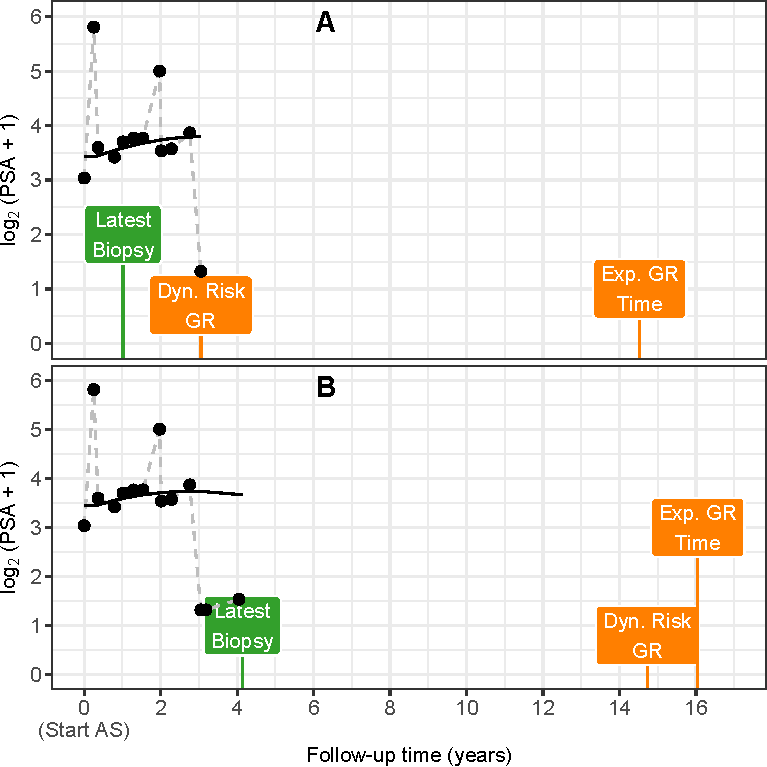
\includegraphics{contents/c2/images/c2_fig2ab.pdf}
\caption{\textbf{Demonstration of personalized schedules at two different visits}. Panels~A and B show fitted (solid black line) versus observed $\log_2 (\mbox{PSA} + 1)$ profile, time of latest biopsy, and personalized time of biopsies for the first demonstration patient. \textbf{Types of personalized schedules}: Exp.~GR~Time schedules a biopsy at the expected time of GR (Gleason reclassification) and Dyn.~Risk~GR schedules a biopsy when the dynamic risk of GR is higher than a certain threshold.}
\label{c2:fig:2ab}
\end{figure}

\begin{figure}
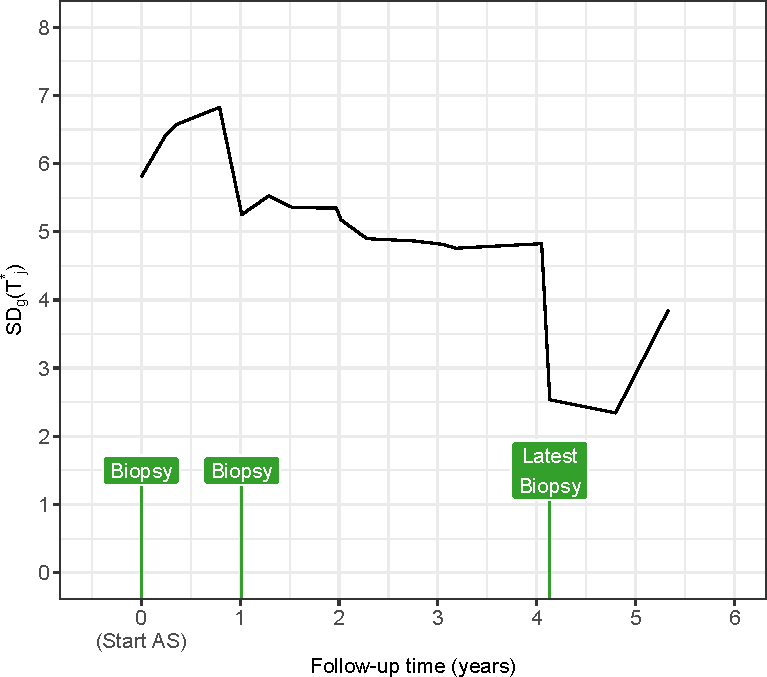
\includegraphics{contents/c2/images/c2_fig2c.pdf}
\caption{History of repeat biopsies and standard deviation ${\mbox{SD}_g(T^*_j) = \sqrt{\mbox{var}_g(T^*_j)}}$ of the posterior predictive distribution of time of Gleason reclassification (see Section~\ref{c2:subsec:ppd_time_to_GR}), over time, for the first demonstration patient.}
\label{c2:fig:2c}
\end{figure}
\section{Simulation Study}
\label{c2:sec:simulation_study}
In Section~\ref{c2:subsec:demo_prias_pers_schedule} we demonstrated that the personalized schedules, schedule future biopsies according to the historical data of each patient. However, we could not perform a full-scale comparison between personalized and PRIAS schedules, because the true time of GR was not known for the PRIAS patients. To this end, we conducted a simulation study comparing personalized schedules with PRIAS and annual schedule, whose details are presented next.

\subsection{Simulation Setup}
\label{c2:subsec:simulation_setup}
The population of AS patients in this simulation study is assumed to have the same entrance criteria as that of PRIAS. The PSA and hazard of GR for these patients follow a joint model of the form postulated in Section~\ref{c2:subsec:jm_fit_prias}, with the only change that $\log_2 \mbox{PSA}$ levels are used as the outcome. The population joint model parameters are equal to the posterior mean of parameters estimated from the corresponding joint model fitted to the PRIAS dataset. We intend to test the efficacy of different schedules for a population which has patients with both faster as well as slowly-progressing PCa. This rate of progression is not only manifested via PSA profiles but also via the baseline hazard. We assume that there are three equal sized subgroups $G_1$, $G_2$ and $G_3$ of patients in the population, each with a baseline hazard from a Weibull distribution, with the following shape and scale parameters $(k, \lambda$): $(1.5, 4)$, $(3, 5)$ and $(4.5, 6)$ for $G_1, G_2$ and $G_3$, respectively. The effect of these parameters is that the mean GR time is lowest in $G_1$ (fast PCa progression) and highest in $G_3$ (slow PCa progression).

From this population, we have sampled 500 datasets with 1000 patients each. We generate a true GR time for each of the patients, and then sample a set of PSA measurements at the same time points as given in PRIAS protocol (quarterly for the first two years of AS, semiannually thereafter). We then split the dataset into a training (750 patients) and a test (250 patients) part, and generate a random and non-informative censoring time for the training patients. We next fit a joint model of the specification given in (\ref{c2:eq:long_model_prias}) and (\ref{c2:eq:hazard_prias}) to each of the 500 training datasets and obtain MCMC samples from the 500 sets of the posterior distribution of the parameters. Using these fitted joint models, we obtain the posterior predictive distribution of time of GR for each of the $500 \times 250$ test patients. This distribution is further used to create personalized biopsy schedules for the test patients. For every test patient we conduct hypothetical biopsies using the following six types of schedules (abbreviated names in parenthesis): personalized schedules based on expected time of GR (Exp.~GR~Time) and median time of GR (Med.~GR~Time), personalized schedules based on dynamic risk of GR (Dyn.~Risk~GR), a hybrid approach between median time of GR and dynamic risk of GR (Hybrid), PRIAS schedule and the annual schedule. The biopsies are conducted as per the algorithm in Figure~\ref{c2:fig:1}. 

To compare the aforementioned schedules we require estimates of the various measures of efficacy described in Section~\ref{c2:sec:choosing_schedule}. To this end, for schedule $S$, we compute pooled estimates of mean offset $E(O^S_j)$ and variance of offset $\mbox{var}(O^S_j)$, as below (estimates for $N^S_j$ are similar):
\begin{align*}
\widehat{E(O^S_j)} &= \frac{\sum_{k=1}^{500} n_k \widehat{E(O^S_k)}}{\sum_{k=1}^{500} n_k}, \\
\widehat{\mbox{var}(O^S_j)} &= \frac{\sum_{k=1}^{500} (n_k - 1) \widehat{\mbox{var}(O^S_k)}}{\sum_{k=1}^{500} (n_k-1)}, 
\end{align*}
where $n_k$ denotes the number of test patients, $\widehat{E(O^S_k)} = {\sum_{l=1}^{n_k}O^S_{kl}}/{n_k}$ is the estimated mean and $\widehat{\mbox{var}(O^S_k)} = {\sum_{l=1}^{n_k}\big\{O^S_{kl} - \widehat{E(O^S_k)}\big\}^2}/(n_k-1)$ is the estimated variance of the offset for the $k$-th simulation. The offset for the $l$-th test patient of the $k$-th dataset is denoted by $O^S_{kl}$.

\subsection{Results}
The pooled estimates of the aforementioned measures are summarized in Table~\ref{c2:table:sim_study_pooled_estimates_all} and Table~\ref{c2:table:sim_study_pooled_estimates_subgroup}. In addition, estimated values of $E(O^S_j)$ are plotted against $E(N^S_j)$ in Figure~\ref{c2:fig:3}. The figure shows that across the schedules, there is an inverse relationship between number $E(O^S_j)$ and $E(N^S_j)$. For example, the annual schedule conducts, on average, 5.2 biopsies to detect GR, which is the highest among all schedules. However, it has the least average offset of 6 months as well. On the other hand, the schedule based on the expected time of GR conducts only 1.9 biopsies on average to detect GR, the least among all schedules, but it also has the highest average offset of 15 months (similar for the median time of GR). Since the annual schedule attempts to contain the offset within a year it has the least $\mbox{SD}(O^S_j) = \sqrt{\mbox{var}(O^S_j)}$. However to achieve this, it conducts a wide range of number of biopsies from patient to patient, i.e., highest $\mbox{SD}(N^S_j) = \sqrt{\mbox{var}(N^S_j)}$. In this regard, schedules based on expected and median time of GR perform the opposite of the annual schedule.

\begin{figure}
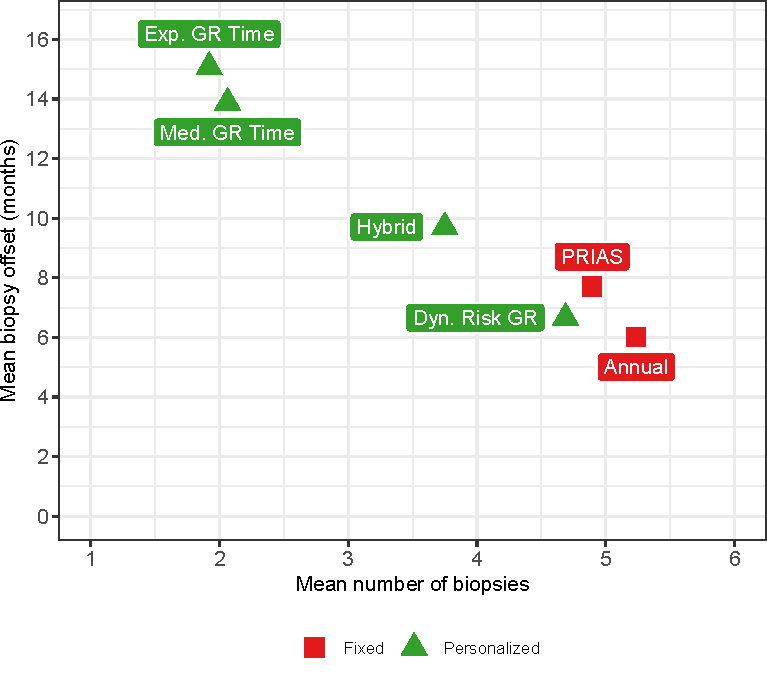
\includegraphics{contents/c2/images/c2_fig3.pdf}
\caption{\textbf{Estimated mean number of biopsies and offset (in months)}. Biopsies are conducted until Gleason reclassification (GR) is detected. Offset is the difference in time at which GR is detected and the true time of GR. Results are based on the simulated (500 datasets) test patients. \textbf{Types of personalized schedules}: Exp.~GR~Time (expected time of GR), Med.~GR~Time (median time of GR), Dyn.~Risk~GR (schedules based on the dynamic risk of GR), Hybrid (a hybrid approach between Med.~GR~Time and Dyn.~Risk~GR). \textbf{Annual}: yearly biopsies. \textbf{PRIAS}: biopsies as per PRIAS protocol.}
\label{c2:fig:3}
\end{figure}

%124781 = 41484 + 41423 + 41874
\begin{table}
\small
\centering
\caption{\textbf{Estimated mean and standard deviation (SD), of the number of biopsies $N^S_j$ and offset $O^S_j$}. Offset (in months) is defined as difference in time at which GR (Gleason reclassification) is detected and the true time of GR. Results are based on all simulated (500 datasets) test patients. \textbf{Types of personalized schedules}: Exp.~GR~Time (expected time of GR), Med.~GR~Time (median time of GR), Dyn.~Risk~GR (schedules based on dynamic risk of GR), Hybrid (a hybrid approach between Med.~GR~Time and Dyn.~Risk~GR). \textbf{Annual}: yearly biopsies. \textbf{PRIAS}: biopsies as per PRIAS protocol.}
\label{c2:table:sim_study_pooled_estimates_all}
\begin{tabular}{lrrrr}
\toprule
Schedule          & $E(N^S_j)$ & $E(O^S_j)$ & ${\mbox{SD}(N^S_j)}$ & ${\mbox{SD}(O^S_j)}$ \\
\midrule
Annual         & 5.24            & 6.01                & 2.53          & 3.46              \\
PRIAS          & 4.90            & 7.71                & 2.36          & 6.31\\
Dyn.~Risk~GR       & 4.69            & 6.66                & 2.19           & 4.38              \\
Hybrid       & 3.75            & 9.70                & 1.71          & 7.25              \\
Med.~GR~Time & 2.06            & 13.88               & 1.41          & 11.80              \\
Exp.~GR~Time & 1.92            & 15.08               & 1.19          & 12.11             \\
\bottomrule
\end{tabular}
\end{table}

\begin{table}
\small
\centering
\caption{\textbf{Subgroup Estimated mean and standard deviation (SD), of the number of biopsies $N^S_j$ and offset $O^S_j$}. Offset (in months) is defined as difference in time at which GR (Gleason reclassification) is detected and the true time of GR. Results based on simulated (500 datasets) test patients, with \textbf{Subgroup $G_1$} and \textbf{Subgroup $G_3$} having the fastest, and slowest progressing cancer patients, respectively. \textbf{Types of personalized schedules}: Exp.~GR~Time (expected time of GR), Med.~GR~Time (median time of GR), Dyn.~Risk~GR (schedules based on dynamic risk of GR), Hybrid (a hybrid approach between Med.~GR~Time and Dyn.~Risk~GR). \textbf{Annual}: yearly biopsies. \textbf{PRIAS}: biopsies as per PRIAS protocol.}
\label{c2:table:sim_study_pooled_estimates_subgroup}
\begin{tabular}{lrrrr}
\toprule
\multicolumn{5}{c}{b) Hypothetical subgroup $G_1$}\\
\midrule
Schedule        & $E(N^S_j)$ & $E(O^S_j)$ & ${\mbox{SD}(N^S_j)}$ & ${\mbox{SD}(O^S_j)}$ \\
\midrule
Annual         & 4.32            & 6.02                & 3.13          & 3.44              \\
PRIAS          & 4.07            & 7.44                & 2.88          & 6.11    \\
Dyn.~Risk~GR       & 3.85            & 6.75                & 2.69          & 4.44              \\
Hybrid       & 3.25            & 10.25               & 2.16          & 8.07              \\
Med.~GR~Time & 1.84            & 20.66               & 1.76          & 14.62             \\
Exp.~GR~Time & 1.72            & 21.65               & 1.47          & 14.75             \\
\midrule     
\multicolumn{5}{c}{c) Hypothetical subgroup $G_2$}\\
\midrule
Schedule        & $E(N^S_j)$ & $E(O^S_j)$ & ${\mbox{SD}(N^S_j)}$ & ${\mbox{SD}(O^S_j)}$ \\
\midrule
Annual         & 5.18            & 5.98                & 2.13          & 3.47              \\
PRIAS          & 4.85            & 7.70                & 2.00          & 6.29        \\
Dyn.~Risk~GR       & 4.63            & 6.66                & 1.82          & 4.37              \\
Hybrid       & 3.68            & 10.32                & 1.37          & 7.45              \\
Med.~GR~Time & 1.89             & 12.33               & 1.16          & 9.44              \\
Exp.~GR~Time & 1.77            & 13.54               & 0.98          & 9.83              \\
\midrule    
\multicolumn{5}{c}{d) Hypothetical subgroup $G_3$}\\
\midrule
Schedule        & $E(N^S_j)$ & $E(O^S_j)$ & ${\mbox{SD}(N^S_j)}$ & ${\mbox{SD}(O^S_j)}$ \\
\midrule
Annual         & 6.20             & 6.02                & 1.76          & 3.46              \\
PRIAS          & 5.76             & 7.98                & 1.71         & 6.51        \\
Dyn.~Risk~GR       & 5.58            & 6.58                & 1.56          & 4.33              \\
Hybrid       & 4.32            & 8.55                & 1.26          & 5.91              \\
Med.~GR~Time & 2.45            & 8.70                & 1.15          & 6.32              \\
Exp.~GR~Time & 2.27            & 10.09               & 0.99          & 7.47              \\
\bottomrule    
\end{tabular}
\end{table}

The PRIAS schedule conducts only 0.3 biopsies less than the annual schedule, but with a higher $\mbox{SD}(O^S_j)$, early detection is not always guaranteed. In comparison, the dynamic risk of GR based schedule performs slightly better than the PRIAS schedule in all four criteria. The hybrid approach combines the benefits of methods with low $E(N^S_j)$ and $\mbox{SD}(N^S_j)$, and methods with low $E(O^S_j)$ and $\mbox{SD}(O^S_j)$. It conducts 1.5 biopsies less than the annual schedule on average, and with a $E(O^S_j)$ of 9.7 months, it detects GR within a year since its occurrence. Moreover, it has both $\mbox{SD}(N^S_j)$ and $\mbox{SD}(O^S_j)$ comparable to PRIAS.

The performance of each schedule differs for the three subgroups $G_1, G_2$, and $G_3$. The annual schedule remains the most consistent across subgroups in terms of the offset, but it conducts two extra biopsies for the subgroup $G_3$ (slowly-progressing PCa) than $G_1$ (faster-progressing PCa). The performance of schedule based on expected time of GR is the most consistent in terms of the number of biopsies, but it detects GR a year later on average in subgroup $G_1$ than $G_3$. For the dynamic risk of GR based schedule and the hybrid schedule, the dynamics are similar to that of the annual schedule. Unlike the latter two schedules, the PRIAS schedule not only conducts more biopsies in $G_3$ than $G_1$ but also detects GR later in $G_3$ than $G_1$.

\begin{figure}
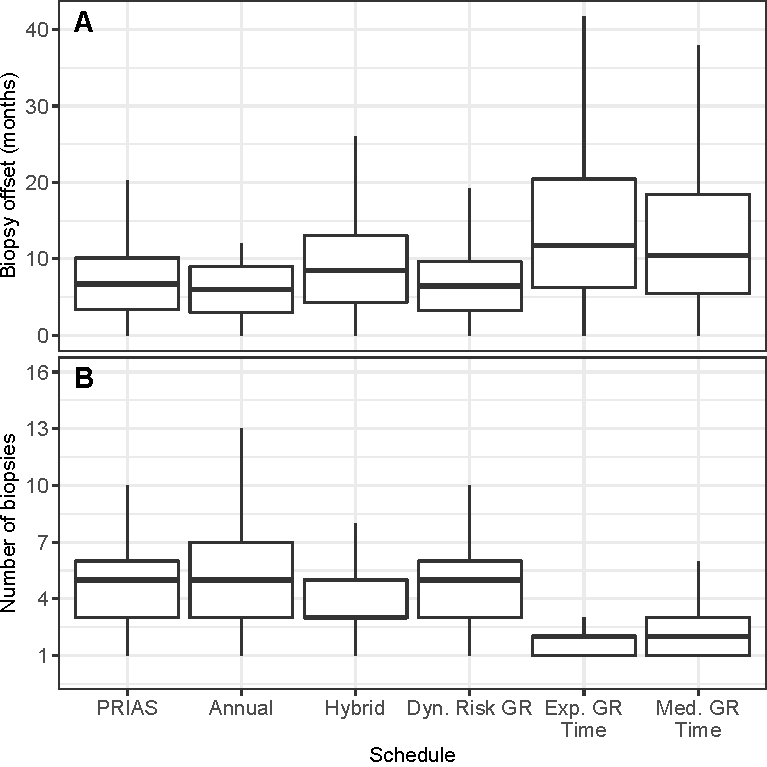
\includegraphics{contents/c2/images/c2_fig4.pdf}
\caption{Variation in the number of biopsies and biopsy offset (difference in time at which Gleason reclassification / GR is detected and the true time of GR, in months). Results are based on the simulated (500 datasets) test patients. Biopsies are conducted until Gleason reclassification (GR) is detected. \textbf{Types of personalized schedules}: Exp.~GR~Time (expected time of GR), Med.~GR~Time (median time of GR), Dyn.~Risk~GR (schedules based on the dynamic risk of GR), Hybrid (a hybrid approach between Med.~GR~Time and Dyn.~Risk~GR). \textbf{Annual}: yearly biopsies. \textbf{PRIAS}: biopsies as per PRIAS protocol.}
\label{c2:fig:4}
\end{figure}

The choice of a suitable schedule using (\ref{c2:eq:loss_func_sim_study_generic}) depends on the chosen measure for evaluation of schedules. In this regard, the schedules we compared either have high $\mbox{SD}(O^S_j)$ and low $\mbox{SD}(N^S_j)$, or vice versa (Table~\ref{c2:table:sim_study_pooled_estimates_all} and Table~\ref{c2:table:sim_study_pooled_estimates_subgroup}). Thus, applying a cutoff on $E(O^S_j)$ when $\mbox{SD}(O^S_j)$ is high may not be as fruitful (same for $N^S_j$) as applying a cutoff on $\mbox{SD}(O^S_j)$ or quantile(s) of $O^S_j$. For example, the schedule based on the dynamic risk of GR is suitable if, on average, the least number of biopsies are to be conducted to detect GR, while simultaneously making sure that at least 90\% of the patients have an average offset less than one year.
\section{Discussion}
\label{c2:sec:discussion}
In this paper, we presented personalized schedules based on joint models for time-to-event and longitudinal data for the surveillance of PCa patients. These schedules are dynamic, and at any given follow-up time, utilize a patient's historical PSA measurements and repeat biopsies conducted up to that time. We proposed two types of personalized schedules, namely those based on expected and median time of GR of a patient, and those based on the dynamic risk of GR. We also proposed a combination (hybrid approach) of these two approaches, which is useful in scenarios where the variance of time of GR for a patient is high. We then proposed criteria for the evaluation of various schedules and a method to select a suitable schedule.

We demonstrated the dynamic and personalized nature of our schedules using the PRIAS dataset. We observed that a recent biopsy impacts the schedules more than recent PSA measurements, which correlates with biopsies being more reliable. Since true GR time is not known for PRIAS patients, we conducted a simulation study to compare personalized schedules with PRIAS and annual schedules. The latter two schedules are already in practice. Hence it can be argued that the maximum possible offsets due to these schedules (one and three years, respectively) are acceptable to doctors. Thus, less frequent schedules with offset under one year may reduce the burden of biopsies while simultaneously being practical. For example, for slowly-progressing patients in our simulation study, we observed that the schedule based on the expected time of GR conducts on average two biopsies and has an average offset of 10 months. In comparison, the annual schedule conducts six biopsies on average and gives an offset smaller by only four months, making the personalized schedule a suitable alternative. For high-risk patients, however, early detection (annual or PRIAS schedule) may be necessary, given the rapidness of progression. When it is not known in advance, if a patient will have a fast or slow-progression of PCa, the hybrid approach may be used. It conducts one biopsy less than the annual schedule in faster-progressing PCa patients and has an average offset of 10.25 months. For slowly-progressing PCa patients, it conducts two biopsies less than the annual schedule and has an average offset of 8.55 months.

More personalized schedules can be added to the current set, using loss functions that asymmetrically penalize overshooting/undershooting the target GR time. For dynamic risk of GR based schedules, more simulations are required to compare data-driven $\kappa$ values (e.g., $\mbox{F}_1$ score), with $\kappa$ chosen using decision analytic approaches such as the net benefit measure~\citep{vickers2006decision}, and with various fixed $\kappa$ values used by doctors in practice. In general, the Gleason scores are susceptible to inter-observer variation~\citep{Gleason_interobs_var}. Schedules that account for error in the measurement of time of GR will be interesting to investigate further~\citep{coley2017}. Lastly, there is potential for including diagnostic information from magnetic resonance imaging (MRI) or DRE. When such information is not continuous, our proposed methodology can be easily extended by utilizing the framework of generalized linear mixed models.

\paragraph{Acknowledgements}
The first and last authors would like to acknowledge support by the Netherlands Organization for Scientific Research's VIDI grant nr. 016.146.301, and Erasmus MC funding. The authors also thank the Erasmus MC Cancer Computational Biology Center for giving access to their IT-infrastructure and software that was used for the computations and data analysis in this study. Lastly, we thank Frank-Jan H. Drost from the Department of Urology, Erasmus University Medical Center, for helping us in accessing the PRIAS data set.

\section*{Appendix}

\begin{subappendices}
\section{Parameter Estimation}
\label{c2:appendix:A}
We estimate parameters of the joint model using Markov chain Monte Carlo (MCMC) methods under the Bayesian framework. Let $\boldsymbol{\theta}$ denote the vector of the parameters of the joint model. The joint model postulates that given the random effects, time to GR and longitudinal responses taken over time are all mutually independent. Under this assumption the posterior distribution of the parameters is given by:
\begin{align*}
p(\boldsymbol{\theta}, \boldsymbol{b} \mid \mathcal{D}_n) & \propto \prod_{i=1}^n p(l_i, r_i, \boldsymbol{y}_i \mid \boldsymbol{b}_i, \boldsymbol{\theta}) p(\boldsymbol{b}_i \mid \boldsymbol{\theta}) p(\boldsymbol{\theta})\\
& \propto \prod_{i=1}^n p(l_i, r_i \mid \boldsymbol{b}_i, \boldsymbol{\theta}) p(\boldsymbol{y}_i \mid \boldsymbol{b}_i, \boldsymbol{\theta}) p(\boldsymbol{b}_i \mid \boldsymbol{\theta}) p(\boldsymbol{\theta}),\\
p(\boldsymbol{b}_i \mid \boldsymbol{\theta}) &= \frac{1}{\sqrt{(2 \pi)^q \text{det}(\boldsymbol{D})}} \exp(\boldsymbol{b}_i^T \boldsymbol{D}^{-1} \boldsymbol{b}_i),
\end{align*}
where the likelihood contribution of longitudinal outcome conditional on random effects is:
\begin{align*}
p(\boldsymbol{y}_i \mid \boldsymbol{b}_i, \boldsymbol{\theta}) &= \frac{1}{\big(\sqrt{2 \pi \sigma^2}\big)^{n_i}} \exp\bigg(-\frac{{\lVert{\boldsymbol{y}_i - \boldsymbol{X}_i\boldsymbol{\beta} - \boldsymbol{Z}_i\boldsymbol{b}_i}\rVert}^2}{\sigma^2}\bigg),\\
\boldsymbol{X}_i &= \{\boldsymbol{x}_i(t_{i1})^T, \ldots, \boldsymbol{x}_i(t_{in_i})^T\}^T,\\
\boldsymbol{Z}_i &= \{\boldsymbol{z}_i(t_{i1})^T, \ldots, \boldsymbol{z}_i(t_{in_i})^T\}^T.
\end{align*}
The likelihood contribution of the time to GR outcome is given by:
\begin{equation}
\label{c2:eq:likelihood_survival_part}
\begin{split}
p(l_i,r_i\mid \boldsymbol{b}_i,\boldsymbol{\theta}) &= \exp\Big\{-\int_0^{l_i} h_i(s \mid \mathcal{M}_i(s), \boldsymbol{w}_i)\mathrm{d}{s}\Big\} \\ & \quad - \exp\Big\{-\int_0^{r_i}h_i(s \mid \mathcal{M}_i(s), \boldsymbol{w}_i)\mathrm{d}{s}\Big\}.
\end{split}
\end{equation}
The integral in (\ref{c2:eq:likelihood_survival_part}) does not have a closed-form solution, and therefore we use a 15-point Gauss-Kronrod quadrature rule to approximate it.

We use independent normal priors with zero mean and variance 100 for the fixed effects $\boldsymbol{\beta}$, and inverse Gamma prior with shape and rate both equal to 0.01 for the parameter $\sigma^2$. For the variance-covariance matrix $\boldsymbol{D}$ of the random effects, we take inverse Wishart prior with an identity scale matrix and degrees of freedom equal to $q$ (number of random effects). For the relative risk model's parameters $\boldsymbol{\gamma}$ and the association parameters $\boldsymbol{\alpha}$, we use independent normal priors with zero mean and variance 100.

\subsection{Parameter Estimates}
The longitudinal evolution of $\log_2 (\mbox{PSA} + 1)$ is modeled with non-linear terms. Hence, the interpretation of the coefficients in this model is not straightforward. Instead of the parameter estimates, in Figure~\ref{c2:fig:app1}, we present the fitted marginal evolution of $\log_2 (\mbox{PSA} + 1)$ over a period of 10 years for a hypothetical patient who is included in AS at the age of 70 years. 

%In addition we present plots of observed versus fitted PSA profiles for nine randomly selected PRIAS patients in Figure~\ref{c2:fig:app2}. Lastly, the quantile-quantile plot of subject-specific residuals in Figure~\ref{c2:fig:app3} shows that the assumption of t-distributed (df=3) errors is reasonably met by the fitted model.

\begin{figure}
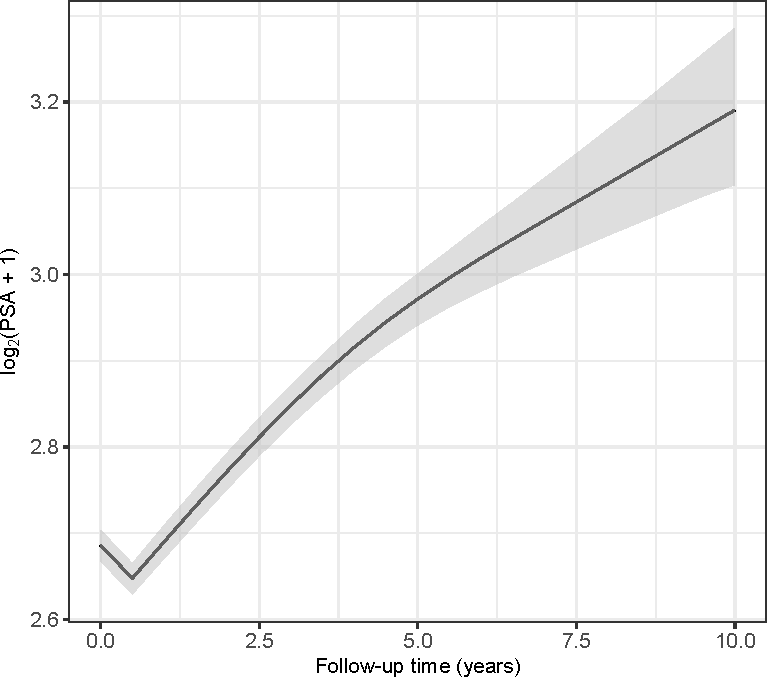
\includegraphics{contents/c2/images/c2_fig_app1.pdf}
\caption{\textbf{Fitted marginal evolution} of $\log_2(\mbox{PSA} + 1)$ measurements over a period of 10 years with 95\% credible interval, for a hypothetical patient who is included in AS at the age of 70 years.}
\label{c2:fig:app1}
\end{figure}

%\begin{figure}
%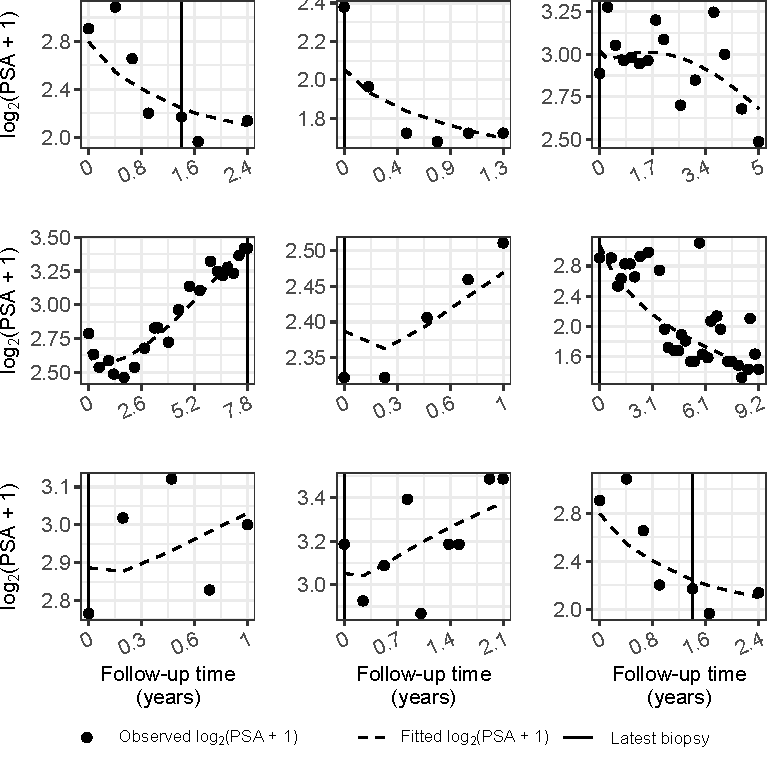
\includegraphics{contents/c2/images/c2_fig_app2.pdf}
%\caption{\textbf{Fitted versus observed} ${\log_2(\mbox{PSA} + 1)}$ profiles for nine randomly selected PRIAS patients. The fitted profiles utilize information from the observed PSA measurements, and time of the latest biopsy.}
%\label{c2:fig:app2}
%\end{figure}

%\begin{figure}
%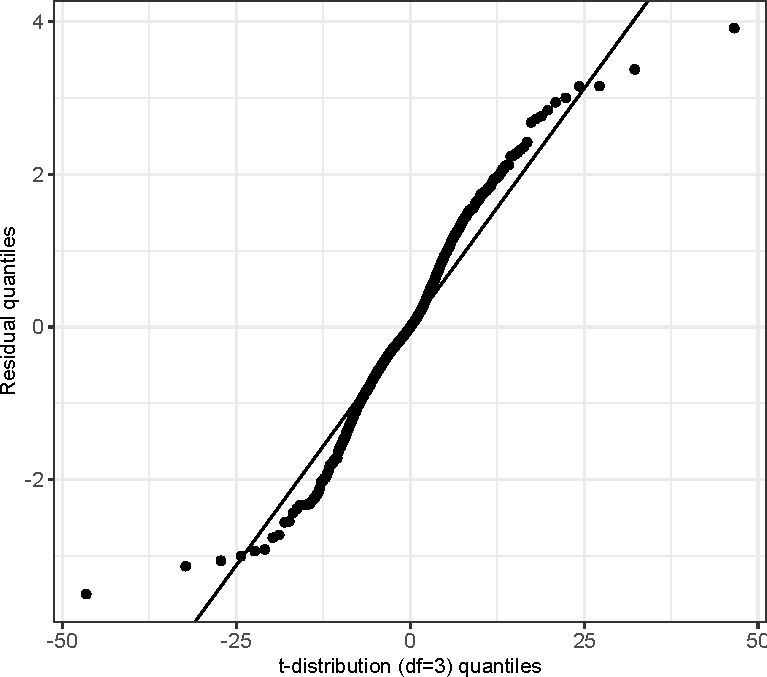
\includegraphics{contents/c2/images/c2_fig_app3.pdf}
%\caption{\textbf{Quantile-quantile plot} of subject-specific residuals of PSA obtained from the joint model fitted to the PRIAS dataset.}
%\label{c2:fig:app3}
%\end{figure}

For the relative risk sub-model, the parameter estimates in Table~\ref{c2:table:app1} show that ${\log_2 (\mbox{PSA} + 1)}$ velocity and the age at the time of inclusion in AS are strongly associated with the hazard of GR. For any patient, an increase in $\log_2 (\mbox{PSA} + 1)$ velocity from -0.061 to 0.136 (first and third quartiles of the fitted velocities, respectively) corresponds to a 2.046 fold increase in the hazard of GR. An increase in age at the time of inclusion in AS from 65 years to 75 years (first and third quartiles of age in PRIAS dataset) corresponds to a 1.428 fold increase in the hazard of GR.

\begin{table}
\small
\centering
\caption{\textbf{Parameters of the relative-risk sub-model}: Estimated mean and 95\% credible interval. Age is median centered.}
\label{c2:table:app1}
\begin{tabular}{lrrrrr}
\toprule
Variable                      & Mean   & Std. Dev & 2.5\%  & 97.5\%                 & P              \\ 
\midrule
$(\mbox{Age} - 70)$                  & 0.036 & 0.006 & 0.024 & 0.047 & \textless0.000 \\
$(\mbox{Age} - 70)^2$   & -0.001 & 0.001 & -0.003 & 7.861 $\times 10^{-5}$ & 0.084          \\
$\log_2 (\mbox{PSA} + 1)$                  & -0.084 & 0.080 & -0.241 & 0.072 & 0.296         \\
Slope($\log_2 (\mbox{PSA} + 1)$)           & 3.580 & 0.403 & 2.815 & 4.373 & \textless0.000 \\
\bottomrule
\end{tabular}
\end{table}

\section{Ascertainment Bias: PSA Doubling Time-Dependent Biopsies and Competing Events}
\label{c2:appendix:B}
\textbf{PSA dependent interval-censored time of upgrading:} The true time of upgrading $T^*_i$ is not known for any of the patients in PRIAS. To detect upgrading, PRIAS uses a fixed schedule of biopsies wherein biopsies are conducted at year one, year four, year seven and year ten of follow-up, and every five years after that. However, PRIAS switches to a more frequent annual biopsy schedule for faster-progressing patients. These are patients with PSA doubling time (PSA-DT) between 0 and 10 years, which is measured as the inverse of the slope of the regression line through the base two logarithm of PSA values. Thus, the interval $l_i < T_i^* \leq r_i$ in which upgrading is detected depends on the observed PSA values. 

\textbf{Competing events:} The primary event of interest in this paper is upgrading observed via a positive biopsy. There are three types of competing events, namely death, removal of patients from AS on the basis of their observed DRE and PSA measurements, watchful-waiting, and loss to follow-up of patients because of patient anxiety or unknown reasons.

The number of patients obtaining the event death is small compared to the number of patients who obtain the primary event upgrading. Hence in this paper, considering death as non-informative censoring may be viable. We also consider the loss to follow-up as non-informative censoring, which may not always be true. This is especially the case when the reason for loss to follow-up is unknown. However, when the reason for loss to follow-up is patient anxiety, it is often on the basis of their observed results. Given the large number of loss to follow-up patients, considering these patients as censored is a limitation of our work. However, the problem of the unknown reason for dropout is not specific to only our model. For the remaining patients who are removed from AS on the basis of their observed longitudinal data (e.g., treatment, watchful-waiting), in the next paragraph, we show that the removal of these patients is non-informative about the parameters of the model for the true time of upgrading.

Given the aforementioned issues of PSA dependent interval censoring and removal of patients on the basis of their observed longitudinal data is natural to question in this scenario if the parameters of the joint model are affected by these two. However, because the parameters of the joint model are estimated using a full likelihood approach~\citep{tsiatis2004joint}, the joint model allows the schedule of biopsies, as well as censoring to depend upon the observed PSA measurements (e.g., via PSA-DT), under the condition that the model is correctly specified. To show this, consider the following full general specification of the joint model that we use. Let $\boldsymbol{y}_i$ denote the observed PSA measurements for the $i$-th patient, and $l_i, r_i$ denote the two time points of the interval in which upgrading occurs for the $i$-th patient. In addition, let $T_i^S$ and $\mathcal{V}_i$ denote the schedule of biopsies, and the schedule PSA measurements, respectively. Let $G^*_i$ denote the time of removal from AS without observing upgrading. Under the assumption that $T_i^S, G^*_i, \mathcal{V}_i$ may depend upon only the observed data $\boldsymbol{y}_i$, the joint likelihood of the various processes is given by:
\begin{equation*}
p(\boldsymbol{y}_i, l_i, r_i, T_i^S, G^*_i, \mathcal{V}_i \mid \boldsymbol{\theta}, \boldsymbol{\psi}) = p(\boldsymbol{y}_i, l_i, r_i \mid \boldsymbol{\theta}) \times p(T_i^S, G^*_i, \mathcal{V}_i \mid \boldsymbol{y}_i, \boldsymbol{\psi}).
\end{equation*}
where, $\boldsymbol{\psi}$ is the vector of parameters for the processes $T_i^S, G^*_i, \mathcal{V}_i$. From this decomposition, we can see that even if the processes $T_i^S, G^*_i, \mathcal{V}_i$ may be determined from $\boldsymbol{y}_i$, if we are interested in the parameters $\boldsymbol{\theta}$ of the joint distribution of longitudinal and event outcomes, we can maximize the likelihood based on the first term and ignore the second term. In other words, the second term will not carry information for $\boldsymbol{\theta}$. Lastly, since we use a full likelihood approach with an interval censoring specification, the estimates that we obtain are consistent and asymptotically unbiased \citep{gentleman1994maximum}, despite the interval censoring observed. 

We also demonstrate the validity of our argument via a simulated dataset of 750 patients. The true event times $T^*_i$ for these patients were generated using parameters from a joint model fitted to the PRIAS dataset (with the only change that $\log_2 \mbox{PSA}$ levels are used as the outcome). However, this joint model did not include the association between the velocity of log PSA values and the hazard of GR. That is, the hazard of GR $h_i(t)$ at any time $t$ was dependent only on the underlying $\log_2 \mbox{PSA}$ value $m_i(t)$ at that time. Furthermore, for these patients, we used the schedule of PRIAS to generate the interval $l_i \leq T^*_i \leq r_i$ in which GR is detected. Thus the observed data for $i$-th patient is $\{\boldsymbol{y}_i, l_i, r_i\}$. Our aim is to show that if there is no association between $h_i(t)$ and velocity of log PSA value $m'_i(t)$, then even though the biopsy schedule depends on PSA-DT (which is a crude measure of PSA velocity), a joint model fitted with both value and velocity associations will have an insignificant velocity association. In the fitted joint model, we found the value association (95\% credible interval in brackets) to be 0.182~[0.090,~0.274], and the velocity association to be -0.001~[-0.295,~0.254]. That is, even though the schedule of biopsies depended upon observed PSA values, it did not lead to a spurious velocity association. 

\section{Source Code}
The source code for fitting the joint model is available at \url{https://raw.githubusercontent.com/anirudhtomer/prias/master/src/chapter2_biometricspaper/Gleason%20as%20event/log2psaplus1_and_pluspt1.R}. 

The code generating the simulation population is available at \url{https://github.com/anirudhtomer/prias/blob/master/src/chapter2_biometricspaper/simulation_study/SimulateJM.R}. 

The code for scheduling biopsies using fixed schedules and utility functions is available at \url{https://github.com/anirudhtomer/prias/blob/master/src/chapter2_biometricspaper/simulation_study/nbAndOffset.R}.

\end{subappendices}

\clearpage
\bibliographystyle{apalike}
\bibliography{c2_bib}
\chapter[Personalized Decision Making for Biopsies in Prostate Cancer Active Surveillance Programs][Personalized Decision Making]{Personalized Decision Making for Biopsies in Prostate Cancer Active Surveillance Programs}
\label{c3}

\vspace*{\fill}
\textbf{This chapter is based on the paper}\\
\underline{Tomer, A.}, Rizopoulos, D., Nieboer, D., Drost, F.J., Roobol, M.J., and Steyerberg, E.W. (2019). Personalized decision making for biopsies in prostate cancer active surveillance programs. \emph{Medical Decision Making}, 39(5): 499--508. doi: \url{https://doi.org/10.1177/0272989X19861963}

\clearpage
\begin{abstract}
\textbf{Background.} Low-risk prostate cancer patients enrolled in active surveillance programs commonly undergo biopsies for examination of cancer progression. Biopsies are conducted as per a fixed and frequent schedule (e.g., annual biopsies). Since biopsies are burdensome, patients do not always comply with the schedule, which increases the risk of delayed detection of cancer progression.

\textbf{Objective.} Our aim is to better balance the number of biopsies (burden) and the delay in detection of cancer progression (less is beneficial), by personalizing the decision of conducting biopsies.

\textbf{Data Sources.} We use patient data of the world's largest active surveillance program (PRIAS). It enrolled 5270 patients, had 866 cancer progressions, and an average of nine prostate-specific antigen (PSA) and five digital rectal examination (DRE) measurements per patient.

\textbf{Methods.} Using joint models for time-to-event and longitudinal data, we model the historical DRE and PSA measurements, and biopsy results of a patient at each follow-up visit. This results in a visit and patient-specific cumulative-risk of cancer progression. If this risk is above a certain threshold, we schedule a biopsy. We compare this personalized approach with the currently practiced biopsy schedules via an extensive and realistic simulation study, based on a replica of the patients from the PRIAS program.

\textbf{Results.} The personalized approach saved a median of six biopsies (median:~4,~IQR:~2--5), compared to the annual schedule (median:~10,~IQR:~3--10). However, the delay in detection of progression (years) is similar for the personalized (median:~0.7,~IQR:~0.3--1.0) and the annual schedule (median:~0.5,~IQR:~0.3--0.8).

\textbf{Conclusions.} We conclude that personalized schedules provide substantially better balance in the number of biopsies per detected progression for men with low-risk prostate cancer.
\end{abstract}
\clearpage
% !TEX root =  ../chapter1.tex
\section{Introduction}
\label{c3:sec:introduction}
Prostate cancer is the second most frequently diagnosed cancer in men worldwide~\citep{GlobalCancerStats2012}. In prostate cancer screening programs, many of the diagnosed tumors are clinically insignificant/over-diagnosed~\citep{etzioni2002overdiagnosis}. To avoid further over-treatment, patients diagnosed with low-grade prostate cancer are commonly advised to join active surveillance (AS) programs. In AS, invasive treatments such as surgery are delayed until cancer progresses. Cancer progression is routinely monitored via serum prostate-specific antigen (PSA) measurements, a protein biomarker; digital rectal examination (DRE) measurements, a measure of the size and location of the tumor; and biopsies.

While larger values for PSA and/or DRE, may indicate cancer progression, biopsies are the most reliable cancer progression examination technique used in AS. When a patient's biopsy Gleason score becomes larger than 6 (positive biopsy, cancer progression detected), AS is stopped, and the patient is advised treatment~\citep{bokhorst2015compliance}. However, biopsies are invasive, painful, and prone to medical complications~\citep{ehdaie2014impact,fujita2009serial}. Hence, they are conducted intermittently until a positive biopsy. Consequently, at the time of a positive biopsy, cancer progression may be observed with a delay of unknown duration. This delay is defined as the difference between the time of the positive biopsy and the unobserved true time of cancer progression. Thus, the decision to conduct biopsies requires a compromise between the burden of biopsy and the potential delay in the detection of cancer progression.

In AS, a delay in the detection of cancer progression around 12 to 14 months is assumed to be unlikely to substantially increase the risk of adverse downstream outcomes~\citep{inoue2018comparative,carvalho}. However, for biopsies, there is little consensus on the time gap between them~\citep{loeb2014heterogeneity,bruinsma2016active,nieboer2018active}. Many AS programs focus on minimizing the delay in the detection of cancer progression by scheduling biopsies annually for all patients. A drawback of annual biopsies, and other currently practiced fixed/heuristic schedules~\citep{loeb2014heterogeneity,bruinsma2016active,nieboer2018active}, is that they ignore the large variation in the time of cancer progression of AS patients. While they may work well for patients who progress early (\emph{fast progressing}) in AS, but for a large proportion of patients who do not progress, or progress late (\emph{slow progressing}) in AS, many unnecessary, burdensome biopsies are scheduled. To mediate the burden between the \emph{fast} and \emph{slow progressing} patients, the world's largest AS program, Prostate Cancer Research International Active Surveillance, PRIAS,~\citep{bokhorst2016decade}, schedules annual biopsies only for patients with a low PSA doubling time~\citep{bokhorst2015compliance}. For everyone else, PRIAS schedules biopsies at following fixed follow-up times: year one, four, seven, and ten, and every five years thereafter. Despite this effort in PRIAS, patients may get scheduled for four to ten biopsies over a period of ten years. Therefore, compliance for biopsies is low in PRIAS~\citep{bokhorst2015compliance}. This can lead to a delay in the detection of cancer progression and reduce the effectiveness of AS.

We aim to better balance the number of biopsies (more are burdensome), and the delay in the detection of cancer progression (less is beneficial), than currently practiced schedules. We intend to achieve this by personalizing the decision to conduct biopsies (see Figure~\ref{c3:fig:1}). These decisions are made at a patient's pre-scheduled follow-up visits for DRE and PSA measurements. To develop the personalized decision-making methodology, we utilize the data of the patients enrolled in the PRIAS study. We model this data and develop the personalized approach using joint models for time-to-event and longitudinal data~\citep{tsiatis2004joint,rizopoulos2012joint}. In order to compare the personalized approach with current schedules, we conduct an extensive simulation study based on a replica of the patients from the PRIAS program. 

\begin{figure}
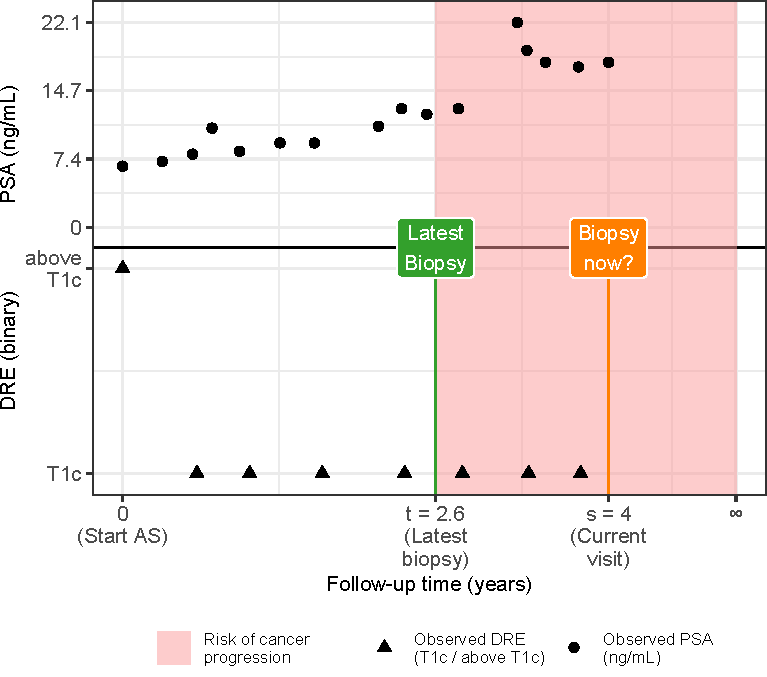
\includegraphics{contents/c3/images/c3_fig1.pdf}
\caption{\textbf{The personalized decision-making problem:} Available data of a patient $j$, who had his latest negative biopsy at $t=2.6$ years. The shaded region shows the time period in which the patient is at risk of cancer progression. His current pre-scheduled follow-up visit for measurement of DRE and PSA is at $s=4$ years. Using his entire history of DRE $\mathcal{Y}_{dj}(s)$ and PSA $\mathcal{Y}_{pj}(s)$ measurements up to the current visit $s$, and the time of the latest biopsy $t$, we intend to make a decision on scheduling a biopsy at the current visit.}
\label{c3:fig:1}
\end{figure}
% !TEX root =  ../c3.tex
\section{Methods}
\label{c3:sec:methods}
\subsection{Study Population}
\label{c3:subsec:study_population}
To develop our methodology, we use the data (see Table~\ref{c3:table:1}) of prostate cancer patients from the world's largest AS study called PRIAS~\citep{bokhorst2016decade}. More than 100 medical centers from 17 countries worldwide contribute to the collection of data, utilizing a common study protocol and a web-based tool, both available at \url{www.prias-project.org}. We use data collected over ten years, between December 2006 (beginning of PRIAS study) and December 2016. The primary event of interest is cancer progression detected upon a positive biopsy. The time of cancer progression is interval-censored because biopsies are scheduled periodically. Biopsies are scheduled as per the PRIAS protocol (see Section~\ref{c3:sec:introduction}). There are three types of competing events, namely death, removal of patients from AS based on their observed DRE and PSA measurements, and loss to follow-up. We assume these three types of events to be censored observations. However, our model allows the removal of patients to depend on observed longitudinal data and baseline covariates of the patient. Under the aforementioned assumption of censoring, Figure~\ref{c3:fig:2} shows the cumulative-risk of cancer progression over the study follow-up period.

\begin{table}
\small
\centering
\caption{\textbf{Summary of the PRIAS dataset}. The primary event of interest is cancer progression. A DRE measurement equal to T1c~\citep{schroder1992tnm} indicates a clinically inapparent tumor which is not palpable or visible by imaging, while tumors with $\mbox{DRE} > \mbox{T1c}$ are palpable. IQR: interquartile range.}
\label{c3:table:1}
\begin{tabular}{lr}
\toprule
Data & Value\\
\midrule
Total patients & 5270\\
Cancer progression (primary event) & 866\\
Loss to follow-up (anxiety or unknown) & 685\\
Removal on the basis of PSA and DRE & 464\\
Death (unrelated to prostate cancer) & 61\\
Death (related to prostate cancer) & 2\\
\midrule
Median Age (years) & 70 (IQR: 65--75)\\
Total PSA measurements & 46015\\
Median number of PSA measurements per patient &  7 (IQR: 5--12)\\
Median PSA value (ng/mL) & 5.6 (IQR: 4.0--7.5)\\
Total DRE measurements & 25606\\
Median number of DRE measurements per patient & 4 (IQR: 3--7)\\
$\mbox{DRE} = \mbox{T1c}$ (\%) & 23538/25606 (92\%) \\
\bottomrule
\end{tabular}
\end{table}

\begin{figure}
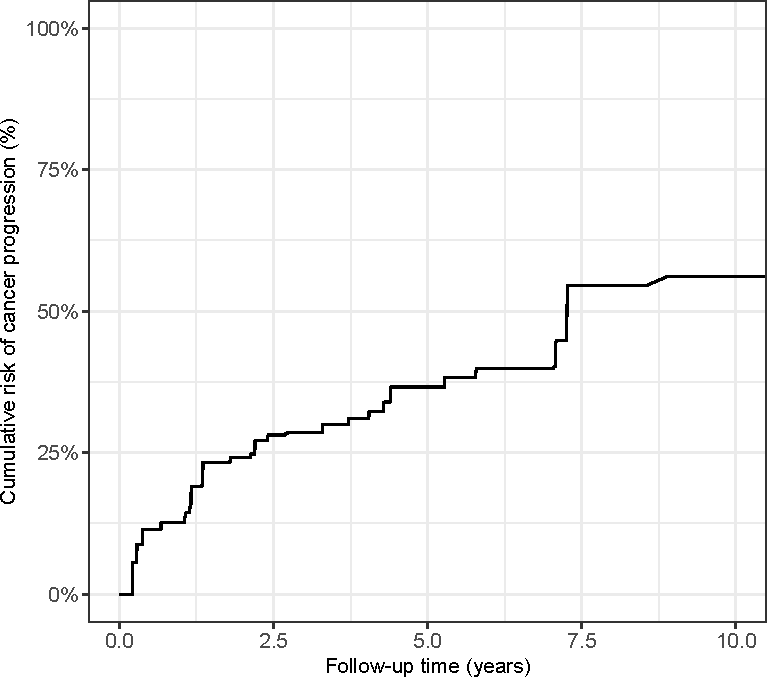
\includegraphics{contents/c3/images/c3_fig2.pdf}
\caption{\textbf{Estimated cumulative-risk of cancer progression in AS} for patients in the Prostate Cancer Research International Active Surveillance (PRIAS) dataset. Nearly 50\% patients (\emph{slow progressing}) do not progress in the ten year follow-up period. Cumulative-risk is estimated using nonparametric maximum likelihood estimation~\citep{turnbull1976empirical}, to account for interval censored cancer progression times observed in the PRIAS dataset. Censoring includes death, removal from AS on the basis of observed longitudinal data, and patient dropout.}
\label{c3:fig:2}
\end{figure}

For all patients, PSA measurements (ng/mL) are scheduled every three months for the first two years and every six months thereafter. The DRE measurements are scheduled every six months. We use the DRE measurements as ${\mbox{DRE} = \mbox{T1c}}$ versus $\mbox{DRE} > \mbox{T1c}$. A DRE measurement equal to T1c~\citep{schroder1992tnm} indicates a clinically inapparent tumor that is not palpable or visible by imaging. In contrast, tumors with $\mbox{DRE} > \mbox{T1c}$ are palpable.

\textbf{Data Accessibility:} The PRIAS database is not openly accessible. However, access to the database can be requested based on a study proposal approved by the PRIAS steering committee. The website of the PRIAS program is \url{www.prias-project.org}.

\subsection{A Bivariate Joint Model for the Longitudinal PSA, and DRE Measurements, and Time of Cancer Progression}
Let $T_i^*$ denote the true cancer progression time of the ${i\mbox{-th}}$ patient included in PRIAS. Since biopsies are conducted periodically, $T_i^*$ is observed with interval censoring ${l_i < T_i^* \leq r_i}$. When progression is observed for the patient at his latest biopsy time $r_i$, then $l_i$ denotes the time of the second latest biopsy. Otherwise, $l_i$ denotes the time of the latest biopsy and ${r_i=\infty}$. Let $\boldsymbol{y}_{di}$ and $\boldsymbol{y}_{pi}$ denote his observed DRE and PSA longitudinal measurements, respectively. The observed data of all $n$ patients is denoted by ${\mathcal{D}_n = \{l_i, r_i, \boldsymbol{y}_{di}, \boldsymbol{y}_{pi}; i = 1, \ldots, n\}}$.

\begin{figure}
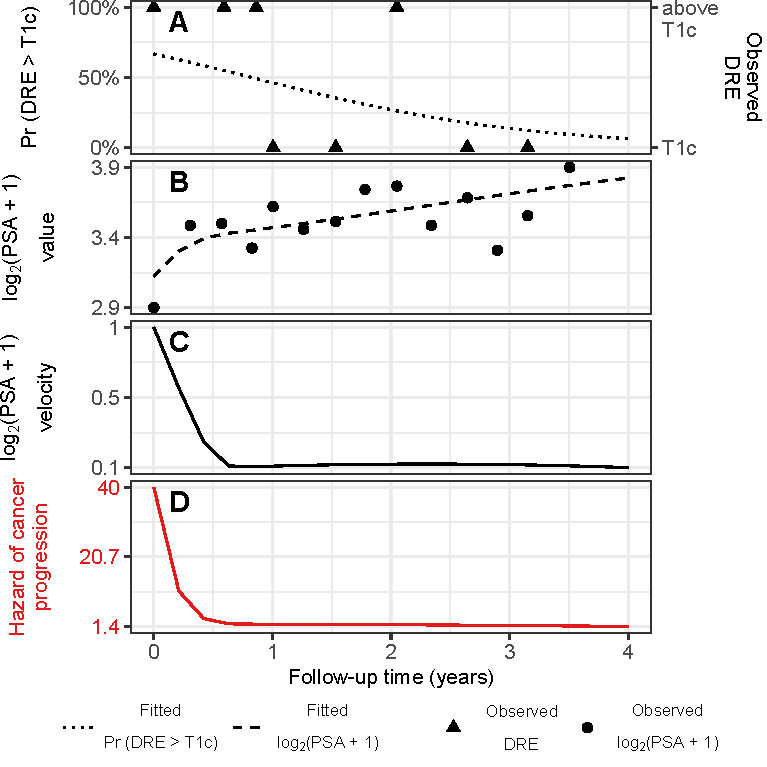
\includegraphics{contents/c3/images/c3_fig3.pdf}
\caption{\textbf{Illustration of the joint model fitted to the PRIAS dataset}. \textbf{Panel~A:} Observed DRE measurements and the fitted probability of obtaining $\mbox{DRE} > \mbox{T1c}$ (\ref{c3:eq:long_model_dre}). \textbf{Panel~B:} Observed and fitted $\log_2(\mbox{PSA} + 1)$ values (\ref{c3:eq:long_model_psa}). \textbf{Panel~C:} Estimated $\log_2(\mbox{PSA} + 1)$ velocity over time. \textbf{Panel~D}: Estimated hazard of cancer progression (\ref{c3:eq:rel_risk_model}). It depends on the fitted log odds of having a $\mbox{DRE} > \mbox{T1c}$, and the fitted $\log_2(\mbox{PSA} + 1)$ value and velocity.}
\label{c3:fig:3}
\end{figure}

In our joint model, the patient-specific DRE and PSA measurements over time are modeled using a bivariate generalized linear mixed effects sub-model. The sub-model for DRE is given by (see~Panel~A, Figure~\ref{c3:fig:3}):
\begin{equation}
\label{c3:eq:long_model_dre}
\begin{split}
    \mbox{logit} \big[\mbox{Pr}\{y_{di}(t) > \mbox{T1c}\}\big] &= \beta_{0d} + b_{0di} + (\beta_{1d} + b_{1di}) t\\
    &+ \beta_{2d} (\mbox{Age}_i-70)  + \beta_{3d} (\mbox{Age}_i-70)^2
    \end{split}
\end{equation}
where, $t$ denotes the follow-up visit time, and $\mbox{Age}_i$ is the age of the ${i\mbox{-th}}$ patient at the time of inclusion in AS. We have centered the Age variable around the median age of 70 years for better convergence during parameter estimation. However, this does not change the interpretation of the parameters corresponding to the Age variable. The fixed effect parameters are denoted by ${\{\beta_{0d}, \ldots, \beta_{3d}\}}$, and ${\{b_{0di}, b_{1di}\}}$ are the patient specific random effects. With this definition, we assume that the patient-specific log odds of obtaining a DRE measurement larger than T1c remain linear over time. 

The mixed effects sub-model for PSA is given by (see~Panel~B, Figure~\ref{c3:fig:3}):
\begin{equation}
\label{c3:eq:long_model_psa}
\begin{split}
    \log_2 \big\{y_{pi}(t) + 1\big\} &= m_{pi}(t) + \varepsilon_{pi}(t),\\
    m_{pi}(t) &= \beta_{0p} + b_{0pi} + \sum_{k=1}^4 (\beta_{kp} + b_{kpi})  B_k(t,\mathcal{K})\\ 
    &+ \beta_{5p} (\mbox{Age}_i-70) + \beta_{6p} (\mbox{Age}_i-70)^2,
    \end{split}
\end{equation}
where, $m_{pi}(t)$ denotes the %underlying
measurement error free value of $\log_2 (\mbox{PSA} + 1)$ transformed~\citep{pearson1994mixed,lin2000latent} measurements at time $t$. We model it non-linearly over time using B-splines~\citep{de1978practical}. To this end, our B-spline basis function $B_k(t, \mathcal{K})$ has 3 internal knots at $\mathcal{K} = \{0.1, 0.7, 4\}$ years, and boundary knots at 0 and 5.42 years (95-th percentile of the observed follow-up times). This specification allows fitting the $\log_2 (\mbox{PSA} + 1)$ levels in a piecewise manner for each patient separately. The internal and boundary knots specify the different time periods (analogously pieces) of this piecewise nonlinear curve. The fixed effect parameters are denoted by ${\{\beta_{0p},\ldots,\beta_{6p}\}}$, and ${\{b_{0pi}, \ldots, b_{4pi}\}}$ are the patient specific random effects. The error $\varepsilon_{pi}(t)$ is assumed to be t-distributed with three degrees of freedom (Figure~\ref{c3:fig:app5}) and scale $\sigma$, and is independent of the random effects. 

To account for the correlation between the DRE and PSA measurements of a patient, we link their corresponding random effects. More specifically, the complete vector of random effects ${\boldsymbol{b}_i = (b_{0di}, b_{1di}, b_{0pi}, \ldots, b_{4pi})^T}$ is assumed to follow a multivariate normal distribution with mean zero and variance-covariance matrix $\boldsymbol{D}$.

To model the impact of DRE and PSA measurements on the risk of cancer progression, our joint model uses a relative risk sub-model. More specifically, the hazard of cancer progression $h_i(t)$ at a time $t$ is given by (see~Panel~D, Figure~\ref{c3:fig:3}):
\begin{equation}
\label{c3:eq:rel_risk_model}
\begin{split}
    h_i(t) &= h_0(t) \exp\Big(\gamma_1 (\mbox{Age}_i-70) + \gamma_2 (\mbox{Age}_i-70)^2\\
    &+\alpha_{1d} \mbox{logit} \big[\mbox{Pr}\{y_{di}(t) > \mbox{T1c}\}\big] + \alpha_{1p} m_{pi}(t) + \alpha_{2p} \frac{\partial m_{pi}(t)}{\partial {t}}\Big),
    \end{split}
\end{equation}
where, $\gamma_1, \gamma_2$ are the parameters for the effect of age. The parameter $\alpha_{1d}$ models the impact of log odds of obtaining a $\mbox{DRE} > \mbox{T1c}$ on the hazard of cancer progression. The impact of PSA on the hazard of cancer progression is modeled in two ways: a) the impact of the error free underlying PSA value $m_{pi}(t)$ (see~Panel~B, Figure~\ref{c3:fig:3}), and b) the impact of the underlying PSA velocity $\partial m_{pi}(t)/\partial {t}$ (see~Panel~C, Figure~\ref{c3:fig:3}). The corresponding parameters are $\alpha_{1p}$ and $\alpha_{2p}$, respectively. Lastly, $h_0(t)$ is the baseline hazard at time $t$, and is modeled flexibly using P-splines~\citep{eilers1996flexible}. More specifically:
\begin{equation*}
\log{h_0(t)} = \gamma_{h_0,0} + \sum_{q=1}^Q \gamma_{h_0,q} B_q(t, \boldsymbol{v}),
\end{equation*}
where $B_q(t, \boldsymbol{v})$ denotes the $q$-th basis function of a B-spline with knots $\boldsymbol{v} = v_1, \ldots, v_Q$ and vector of spline coefficients $\gamma_{h_0}$. To avoid choosing the number and position of knots in the spline, a relatively high number of knots (e.g., 15 to 20) are chosen and the corresponding B-spline regression coefficients $\gamma_{h_0}$ are penalized using a differences penalty~\citep{eilers1996flexible}.The detailed specification of the baseline hazard $h_0(t)$, and the joint parameter estimation of the two sub-models using the Bayesian approach (R package \textbf{JMbayes}) are presented in Appendix~\ref{c3:appendix:A}.

\subsection{Personalized Decisions for Biopsy}
\label{c3:subsec:pers_decision_making}
Let us assume that a decision of conducting a biopsy is to be made for a new patient $j$ shown in Figure~\ref{c3:fig:1}, at his current follow-up visit time $s$. Let $t\leq s$ be the time of his latest negative biopsy. Let $\mathcal{Y}_{dj}(s)$ and $\mathcal{Y}_{pj}(s)$ denote his observed DRE and PSA measurements up to the current visit, respectively. From the observed measurements we want to extract the underlying measurement error free trend of $\log_2 (\mbox{PSA} + 1)$ values and velocity, and the log odds of obtaining $\mbox{DRE} > \mbox{T1c}$. We intend to combine them to inform us when the cancer progression is to be expected, and to further guide the decision making on whether to conduct a biopsy at the current follow-up visit. The combined information is given by the following posterior predictive distribution $g(T^*_j)$ of his time of cancer progression $T^*_j > t$:
\begin{equation}
\label{c3:eq:post_pred_dist}
g(T^*_j) = p\big\{T^*_j \mid T^*_j > t, \mathcal{Y}_{dj}(s), \mathcal{Y}_{pj}(s), \mathcal{D}_n\big\}.
\end{equation}
The distribution $g(T^*_j)$ is not only patient-specific, but also updates as extra information is recorded at future follow-up visits.

\begin{figure}
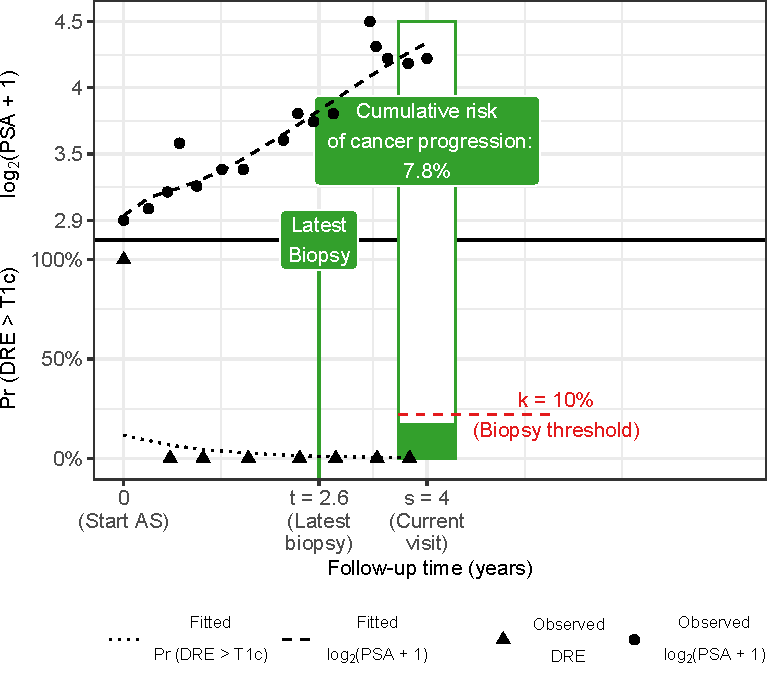
\includegraphics{contents/c3/images/c3_fig4a.pdf}
\caption{\textbf{Personalized decision biopsy not recommended}: Biopsy is recommended only if the personalized cumulative-risk of cancer progression estimated from the joint model fitted to the observed data of the $j$-th patient, is higher than the example risk threshold for biopsy ($\kappa=$ 10\%). The cumulative-risk of cancer progression at the current visit time ($s=$ 4 years) is 7.8\%.}
\label{c3:fig:4a}
\end{figure}

\begin{figure}
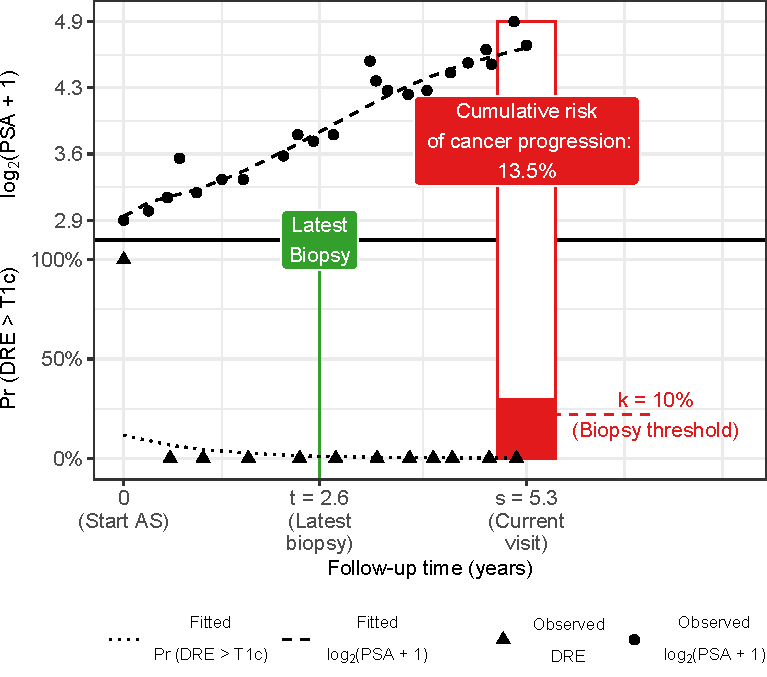
\includegraphics{contents/c3/images/c3_fig4b.pdf}
\caption{\textbf{Personalized decision of biopsy recommended}: Biopsy is recommended only if the personalized cumulative-risk of cancer progression estimated from the joint model fitted to the observed data of the $j$-th patient, is higher than the example risk threshold for biopsy ($\kappa=$ 10\%). The cumulative-risk of cancer progression at the current visit time ($s=$ 5.3 years) is 13.5\%.}
\label{c3:fig:4b}
\end{figure}

A key ingredient in the decision of conducting a biopsy for patient $j$ at the current follow-up visit time $s$ is the personalized cumulative-risk of observing a cancer progression at time $s$ (illustrated in Figure~\ref{c3:fig:4a}, and Figure~\ref{c3:fig:4b}). This risk can be derived from the posterior predictive distribution $g(T^*_j)$~\citep{rizopoulos2011dynamic}, and for $s \geq t$ it is given by:
\begin{equation}
\label{c3:eq:dynamic_risk_prob}
R_j(s \mid t) = \mbox{Pr}\big\{T^*_j \leq s \mid T^*_j > t, \mathcal{Y}_{dj}(s), \mathcal{Y}_{pj}(s), \mathcal{D}_n\big\}.
\end{equation}
A simple and straightforward approach to decide upon conducting a biopsy for patient $j$ at the current follow-up visit would be to do so if his personalized cumulative-risk of cancer progression at the visit is higher than a certain threshold $0 \leq \kappa \leq 1$. For example, as shown in Figure~\ref{c3:fig:4a}, and Figure~\ref{c3:fig:4b}, biopsy at a visit may be scheduled if the personalized cumulative-risk is higher than 10\% (example risk threshold). This decision making process is iterated over the follow-up period, incorporating on each subsequent visit the newly observed data, until a positive biopsy is observed. Subsequently, an entire personalized schedule of biopsies for each patient can be obtained.

The choice of the risk threshold dictates the schedule of biopsies and has to be made on each subsequent follow-up visit of a patient. In this regard, a straightforward approach is choosing a fixed risk threshold, such as 5\% or 10\% risk, at all follow-up visits. Fixed risk thresholds may be chosen by patients and/or doctors according to how they weigh the relative harms of doing an unnecessary biopsy versus a missed cancer progression (e.g., 10\% threshold means a 1:9 ratio) if the biopsy is not conducted~\citep{vickers2006decision}. An alternative approach is that at each follow-up visit, a unique threshold is chosen on the basis of its classification accuracy. More specifically, given the time of latest biopsy $t$ of patient $j$, and his current visit time $s$\, we find a visit-specific biopsy threshold $\kappa$, which gives the highest cancer progression detection rate (true positive rate, or TPR) for the period $(t, s]$. However, we also intend to balance for unnecessary biopsies (high false-positive rate), or a low number of correct detections (high false-negative rate) when the false positive rate is minimized. An approach to mitigating these issues is to maximize the TPR and positive predictive value (PPV) simultaneously. To this end, we utilize the $\mbox{F}_1$~score, which is a composite of both TPR and PPV [estimated as in~\citet{landmarking2017}] and is defined as: 
\begin{equation}
\label{c3:eq:F1_TPR_PPV}
\begin{split}
\mbox{F}_1(t,  s, \kappa) &= 2\frac{\mbox{TPR}(t,  s, \kappa)\ \mbox{PPV}(t,  s, \kappa)}{\mbox{TPR}(t,  s, \kappa) + \mbox{PPV}(t,  s, \kappa)},\\
\mbox{TPR}(t,  s, \kappa) &= \mbox{Pr}\big\{R_j(s \mid t) > \kappa \mid t < T^*_j \leq s\big\},\\
\mbox{PPV}(t,  s, \kappa) &= \mbox{Pr}\big\{t < T^*_j \leq s \mid R_j(s \mid t) > \kappa \big\},
\end{split}
\end{equation}
where, $\mbox{TPR}(t,  s, \kappa)$ and $\mbox{PPV}(t,  s, \kappa)$ are the time-dependent true positive rate and positive predictive value, respectively. These values are unique for each combination of the time period $(t, s]$ and the risk threshold $\kappa$ that is used to discriminate between the patients whose cancer progresses in this time period versus the patients whose cancer does not progress. The same holds true for the resulting $\mbox{F}_1$~score denoted by $\mbox{F}_1(t,  s, \kappa)$. The $\mbox{F}_1$~score ranges between 0 and 1, where a value equal to 1 indicates perfect TPR and PPV. Thus the highest $\mbox{F}_1$~score is desired in each time period $(t, s]$. This can be achieved by choosing a risk threshold $\kappa$, which maximizes $\mbox{F}_1(t, s, \kappa)$. That is, during a patient's visit at time $s$, given that his latest biopsy was at the time $t$, the visit-specific risk threshold to decide a biopsy is given by ${\kappa=\argmax_{\kappa} \mbox{F}_1(t, s, \kappa)}$. The criteria on which we evaluate the personalized schedules based on fixed and visit-specific risk thresholds is the total number of biopsies scheduled, and the delay in detection of cancer progression (details in \hyperref[sec:results]{Results}). 

\subsection{Simulation Study}
\label{c3:subsec:sim_study}
Although the personalized decision-making approach is motivated by the PRIAS study, it is not possible to evaluate it directly on the PRIAS dataset. This is because the patients in PRIAS have already had their biopsies as per the PRIAS protocol. In addition, the true time of cancer progression is interval or right-censored for all patients, making it impossible to correctly estimate the delay in the detection of cancer progression due to a particular schedule. To this end, we conduct an extensive simulation study to find the utility of personalized, PRIAS, and fixed/heuristic schedules. For a realistic comparison, we simulate patient data from the joint model fitted to the PRIAS dataset. The simulated population has the same ten year follow-up period as the PRIAS study. In addition, the estimated relations between DRE and PSA measurements, and the risk of cancer progression are retained in the simulated population.

From this population, we first sample 500 datasets, each representing a hypothetical AS program with 1000 patients in it. We generate a true cancer progression time for each of the ${\mbox{500} \times \mbox{1000}}$ patients and then sample a set of DRE and PSA measurements at the same follow-up visit times as given in PRIAS protocol. We then split each dataset into training (750 patients) and test (250 patients) parts, and generate a random and non-informative censoring time for the training patients. We next fit a joint model of the specification given in~(\ref{c3:eq:long_model_dre}),~(\ref{c3:eq:long_model_psa}),~and~(\ref{c3:eq:rel_risk_model}) to each of the 500 training datasets and obtain MCMC samples from the 500 sets of the posterior distribution of the parameters. 

In each of the 500 hypothetical AS programs, we utilize the corresponding fitted joint models to develop cancer progression risk profiles for each of the ${\mbox{500} \times \mbox{250}}$ test patients. We make the decision of biopsies for patients at their pre-scheduled follow-up visits for DRE and PSA measurements (see Section~\ref{c3:subsec:study_population}), on the basis of their estimated personalized cumulative-risk of cancer progression. These decisions are made iteratively until a positive biopsy is observed. A recommended gap of one year between consecutive biopsies~\citep{bokhorst2015compliance} is also maintained. Subsequently, for each patient, an entire personalized schedule of biopsies is obtained.

We evaluate and compare both personalized and currently practiced schedules of biopsies in this simulation study. A comparison of the schedules is based on the number of biopsies scheduled and the corresponding delay in the detection of cancer progression. We evaluate the following currently practiced fixed/heuristic schedules: biopsy annually, biopsy every one and a half years, biopsy every two years, and biopsy every three years. We also evaluate the biopsy schedule of the PRIAS program (see Section~\ref{c3:sec:introduction}). For the personalized biopsy schedules, we evaluate schedules based on three fixed risk thresholds: 5\%, 10\%, and 15\%, corresponding to a missed cancer progression being 19, 9, and 5.5 times more harmful than an unnecessary biopsy~\citep{vickers2006decision}, respectively. We also implement a personalized schedule wherein for each patient, visit-specific risk thresholds are chosen using $\mbox{F}_1$~score.
% !TEX root = ../c3.tex

\section{Results}
\label{c3:sec:results}
From the joint model fitted to the PRIAS dataset, we found that both $\log_2 \{\mbox{PSA} + 1\}$ velocity, and log odds of having $\mbox{DRE} > \mbox{T1c}$ were significantly associated with the hazard of cancer progression. For any patient, an increase in $\log_2 \{\mbox{PSA} + 1\}$ velocity from -0.03 to 0.16 (first and third quartiles of the fitted velocities, respectively) corresponds to a 1.94 fold increase in the hazard of cancer progression. Whereas, an increase in odds of $\mbox{DRE} > \mbox{T1c}$ from -6.650 to -4.356 (first and third quartiles of the fitted log-odds, respectively) corresponds to a 1.40 fold increase in the hazard of cancer progression. Detailed results pertaining to the fitted joint model are presented in Appendix~\ref{c3:appendix_subsec:A_paramestimates}.

\subsection{Comparison of Various Approaches for Biopsies}
From the simulation study, we obtain the number of biopsies and the delay in detection of cancer progression for each of the ${\mbox{500} \times \mbox{250}}$ test patients using different schedules. Figure~\ref{c3:fig:5} shows that the personalized and PRIAS approaches fall in the region of a better balance between the median number of biopsies and the median delay than fixed/heuristic schedules. Next evaluate these schedules on the basis of both median and interquartile range (IQR) of the number of biopsies and delay (see Figure~\ref{c3:fig:6}). For brevity, only the most widely used annual and PRIAS schedules, the proposed personalized approach with fixed risk thresholds of 5\% and 10\%, and visit-specific threshold chosen using $\mbox{F}_1$ score are discussed next (see~Table~\ref{c3:table:app3} for remaining).

\begin{figure}
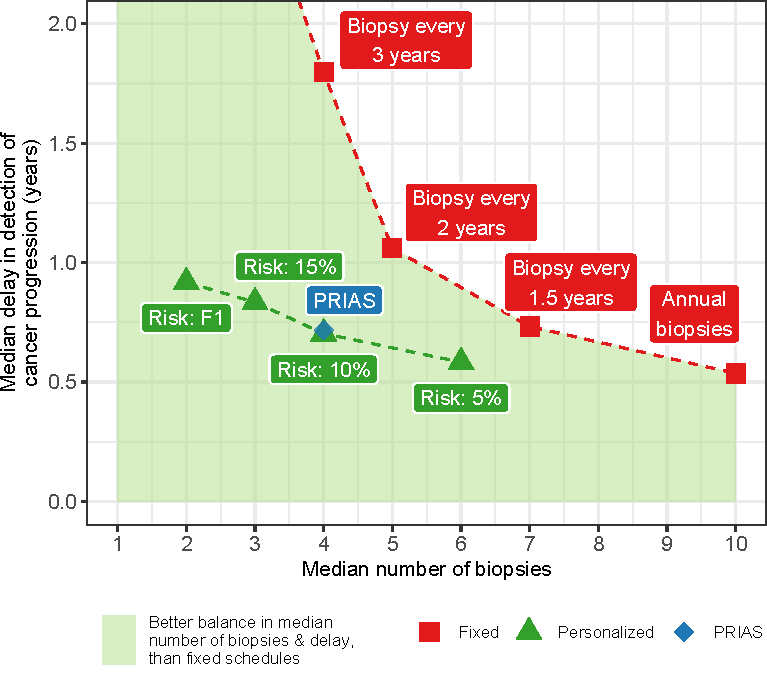
\includegraphics{contents/c3/images/c3_fig5.pdf}
\caption{\textbf{Burden-biopsy frontier:} Median number of biopsies (X-axis), and median delay in detection of cancer progression, in years (Y-axis), estimated from the simulation study. \textbf{Personalized schedules:} Risk:~15\%, Risk:~10\%, and Risk:~5\% approaches, schedule a biopsy if the cumulative-risk of cancer progression at a visit is more than 15\%, 10\%, and 5\%, respectively. Risk:~F1 works similarly, except that it utilizes a visit-specific threshold (see Section~\ref{c3:subsec:pers_decision_making}). The green shaded region depicts the region of better balance in the median number of biopsies and median delay than the currently practiced fixed/heuristic schedules.}
\label{c3:fig:5}
\end{figure}

Since patients have varying cancer progression speeds, the impact of each schedule also varies with it. To highlight these differences, we divide results for three types of patients, as per their time of cancer progression. They are \emph{fast, intermediate,} and \emph{slow progressing} patients. Although such a division may be imperfect and can only be done retrospectively in a simulation setting, we show results for these three groups for illustration. Roughly 50\% of the patients did not obtain cancer progression in the ten year follow-up period of the simulation study. We assume these patients to be \emph{slow progressing} patients. We assume \emph{fast progressing} patients are the ones with an initially misdiagnosed state of cancer~\citep{cooperberg2011outcomes} or high-risk patients who choose AS instead of immediate treatment upon diagnosis. These are roughly 30\% of the population, having a cancer progression time less than 3.5 years. We label the remaining 20\% patients as \emph{intermediate progressing} patients. 

\begin{figure}
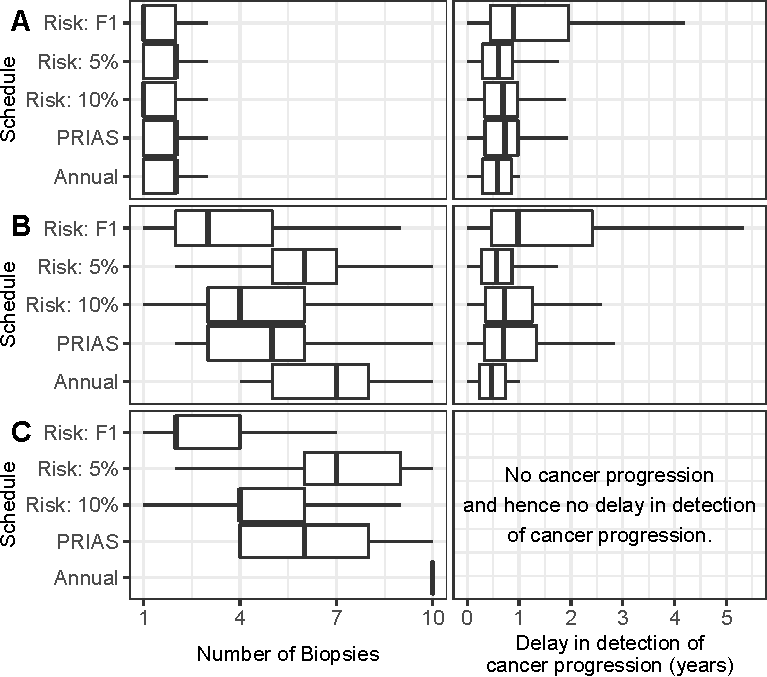
\includegraphics{contents/c3/images/c3_fig6.pdf}
\caption{Variation in the number of biopsies, and the delay in detection of cancer progression, in years, for various biopsy schedules. \textbf{Panel~A:} simulated patients with cancer progression times between 0 and 3.5 years (\emph{fast progressing}). \textbf{Panel~B:} simulated patients with progression times between 3.5 and 10 years (\emph{intermediate progressing}). \textbf{Panel~C:} simulated patients who did not have cancer progression in the ten years of follow-up (\emph{slow progressing}). \textbf{Personalized schedules:} Risk:~10\% approach schedules a biopsy at a visit if the corresponding cumulative-risk of cancer progression is more than 10\%. Risk:~5\% and Risk:~F1 work similarly, except that a visit-specific threshold is used in the latter (see Section~\ref{c3:subsec:pers_decision_making}). \textbf{Annual:} Yearly biopsies, and \textbf{PRIAS:} biopsies as per PRIAS protocol (see Section~\ref{c3:sec:introduction}).}
\label{c3:fig:6}
\end{figure}

For \emph{fast progressing} patients (Panel~A,~Figure~\ref{c3:fig:6}), we note that the personalized schedules with a fixed 10\% risk threshold and visit-specific threshold chosen using $\mbox{F}_1$ score, reduce one biopsy for 50\% of the patients, compared to PRIAS and annual schedule. Despite this, the delay (years) is similar for the personalized schedule with fixed 10\% risk threshold (median:~0.7,~IQR:~0.3--1.0), and the commonly used annual (median:~0.6,~IQR:~0.3--0.9) and PRIAS (median:~0.7,~IQR:~0.3--1.0) schedules.

For \emph{intermediate progressing} patients (Panel~A,~Figure~\ref{c3:fig:6}), we note that the delay (years) due to personalized schedule with fixed 5\% risk threshold (median:~0.6,~IQR:~0.3--0.9) is comparable to that of annual schedule (median 0.5,~IQR:~0.2--0.7). However, it schedules fewer biopsies (median:~6,~IQR:~5--7) than the annual schedule (median:~7,~IQR:~5--8). The delay (years) for PRIAS (median:~0.7,~IQR:~0.3--1.3) and personalized schedule with fixed 10\% risk (median:~0.7,~IQR:~0.4--1.3) are similar, but the personalized approach schedules one less biopsy for 50\% of the patients. Although the approach with the visit-specific risk threshold chosen using $\mbox{F}_1$ score schedules fewer biopsies than the 10\% fixed risk approach, it also has a higher delay.

The patients who are at the most advantage with the personalized schedules are the \emph{slow progressing} patients. These are a total of 50\% patients who did not progress during the entire study. Hence, the delay is not available for these patients (Panel~C of Figure~\ref{c3:fig:6}). For all of these patients, the annual schedule leads to 10 (unnecessary) biopsies. The schedule of the PRIAS program schedules a median of six biopsies (IQR:~4--8). In comparison, the biopsies scheduled by the personalized schedules using fixed 10\% risk threshold (median:~4,~IQR:~4--6) and visit-specific risk chosen using $\mbox{F}_1$ score (median:~2,~IQR:~2--4), are much fewer.

Overall, we observed that the personalized schedule which uses a 10\% risk threshold at all follow-up visits is dominant over the PRIAS schedule, biennial schedule of biopsies, and biopsies every one and a half years (see~Table~\ref{c3:table:app3} for the latter two schedules). This personalized schedule not only schedules fewer biopsies than the aforementioned currently practiced schedules, but the delay in the detection of cancer progression is also either equal or less. The personalized schedule, which uses the risk threshold chosen based on classification accuracy ($\mbox{F}_1$ score) is dominant over the triennial schedule of biopsies. The personalized schedule which uses a 5\% risk threshold schedules fewer biopsies than the annual schedule, while the delay is only trivially more than the annual schedule.
\section{Discussion}
\label{c3:sec:discussion}
We proposed a methodology which better balances the number of biopsies, and the delay in detection of cancer progression than the currently practiced biopsy schedules, for low-risk prostate cancer patients enrolled in active surveillance (AS) programs. The proposed methodology combines a patient's observed DRE and PSA measurements, and the time of the latest biopsy, into a personalized cancer progression risk function. If the cumulative-risk of cancer progression at a follow-up visit is above a certain threshold, then a biopsy is scheduled. We conducted an extensive simulation study, based on a replica of the patients from the PRIAS program, to compare this personalized approach for biopsies with the currently practiced biopsy schedules. We found personalized schedules to be dominant over many of the current biopsy schedules (see Section~\ref{c3:sec:results}).

The main reason for the better performance of personalized schedules is that they account for the variation in cancer progression rate between patients, and also over time within the same patient. In contrast, the existing fixed/heuristic schedules ignore that roughly 50\% of the patients never progress in the first ten years of follow-up (\emph{slow progressing} patients) and do not require biopsies. The \emph{fast progressing} patients require early detection. However, existing methods of identifying these patients, such as the use of PSA doubling time in PRIAS, inappropriately assume that PSA evolves linearly over time. Thus, they may not correctly identify such patients. The personalized approach, however, models the PSA profiles non-linearly. Furthermore, it appends information from PSA with information from DRE and previous biopsy results and combines them into a single cancer progression risk function. The risk function is a finer quantitative measure than individual data measurements observed for the patients. In comparison to decision making with flowcharts, the risk as a single measure of a patient's underlying state of cancer may facilitate shared decision making for biopsies.

Existing work on reducing the burden of biopsies in AS primarily advocates less frequent heuristic schedules (e.g., biopsies biennially instead of annually) of biopsies~\citep{inoue2018comparative}. To our knowledge, risk-based biopsy schedules have barely been explored yet in AS~\citep{nieboer2018active,bruinsma2016active}. The part of our results pertaining to the fixed/heuristic schedules is comparable with corresponding results obtained in existing work~\citep{inoue2018comparative}, even though the AS cohorts are not the same. Thus, we anticipate similar validity for the results pertaining to the personalized schedules.

A limitation of the personalized approach is that the choice of risk threshold is not straightforward, as different thresholds lead to different combinations of the number of biopsies and the delay in the detection of cancer progression. An approach is to choose a risk threshold that leads to personalized schedule dominant (e.g., 10\% risk) over the currently practiced schedules, for a given delay. Since personalized biopsy schedules are less burdensome, they may lead to better compliance. A second limitation is that the results that we presented are valid only in a ten year follow-up period, whereas prostate cancer is a slowly progressing disease. Thus more detailed results, especially for \emph{slow progressing} patients, cannot be estimated. However, very few AS cohorts have a longer follow-period than PRIAS~\citep{bruinsma2016active}. In a screening setting, often the ethno-racial background of the patient, as well as the history of cancer in first degree relatives, are checked. Our model does not take into account either. The reason is that the history of cancer in relatives been found to be predictive of cancer progression only in African-American patients~\citep{goh2013clinical,telang2017prostate}. This is also evident by the fact that PRIAS and many other surveillance programs do not utilize this information in their biopsy protocols~\citep{bokhorst2016decade,nieboer2018active}. In addition, patients who have a higher risk of an aggressive form of cancer are usually not recommended active surveillance. Hence the proposed model is relevant only for low-risk prostate cancer patients eligible for active surveillance. An exception is the active surveillance patients who are old and/or have comorbid illnesses. Currently, such patients may be removed from active surveillance and are instead offered the less intensive watchful waiting~\citep{bokhorst2016decade} option. It is also possible to model watchful waiting as a competing risk in our model. However, this falls outside the scope of the current work because cancer progression, as detected via biopsy, is the standard trigger for treatment advice. Lastly, our results are not valid when the patient data is missing not at random (MNAR).

There are multiple ways to extend the personalized decision-making approach. For example, biopsy Gleason grading is susceptible to inter-observer variation~\citep{coley2017}. Thus accounting for it in our model will be interesting to investigate further. To improve the decision making methodology, future consequences of a biopsy can be accounted for in the model by combining Markov decision processes with joint models for time-to-event and longitudinal data. There is also a potential for including diagnostic information from magnetic resonance imaging (MRI), such as the volume of the prostate tumor as a longitudinal measurement in our model. The resulting predictions can be used to decide the time of the next MRI as well as to make a decision of biopsy. The same holds true for the quality of life measures as well. However, given the scarceness of both MRI and quality of life measurements in the dataset, including them in the current model may not be feasible. We intend further to validate our results in a multi-center AS cohort and subsequently develop a web application to assist in making shared decisions for biopsies.

\paragraph{Acknowledgements}
The first and last Authors would like to acknowledge support by Nederlandse Organisatie voor Wetenschappelijk Onderzoek (the national research council of the Netherlands) VIDI grant nr. 016.146.301, and Erasmus University Medical Center funding. The Authors also thank the Erasmus University Medical Center's Cancer Computational Biology Center for giving access to their IT-infrastructure and software that was used for the computations and data analysis in this study. Lastly, we thank Joost Van Rosmalen from the Department of Biostatistics, Erasmus University Medical Center for feedback on the manuscript.

\paragraph{Conflict of Interest}
The Authors declare that there is no conflict of interest.

\section*{Appendix}

\begin{subappendices}
\section{Parameter Estimation}
\label{c3:appendix:A}
We estimate the parameters of the joint model using Markov chain Monte Carlo (MCMC) methods under the Bayesian framework. Let $\boldsymbol{\theta}$ denote the vector of all of the parameters of the joint model. The joint model postulates that given the random effects, the time to cancer progression, and the DRE and PSA measurements taken over time are all mutually independent. Under this assumption the posterior distribution of the parameters is given by:
\begin{align*}
p(\boldsymbol{\theta}, \boldsymbol{b} \mid \mathcal{D}_n) & \propto \prod_{i=1}^n p(l_i, r_i, \boldsymbol{y}_{di}, \boldsymbol{y}_{pi}, \mid \boldsymbol{b}_i, \boldsymbol{\theta}) p(\boldsymbol{b}_i \mid \boldsymbol{\theta}) p(\boldsymbol{\theta})\\
& \propto \prod_{i=1}^n p(l_i, r_i \mid \boldsymbol{b}_i, \boldsymbol{\theta}) p(\boldsymbol{y}_{di} \mid \boldsymbol{b}_i, \boldsymbol{\theta}) p(\boldsymbol{y}_{pi} \mid \boldsymbol{b}_i, \boldsymbol{\theta}) p(\boldsymbol{b}_i \mid \boldsymbol{\theta}) p(\boldsymbol{\theta}),\\
p(\boldsymbol{b}_i \mid \boldsymbol{\theta}) &= \frac{1}{\sqrt{(2 \pi)^q \text{det}(\boldsymbol{D})}} \exp(\boldsymbol{b}_i^T \boldsymbol{D}^{-1} \boldsymbol{b}_i),
\end{align*}
where, the likelihood contribution of the DRE outcome, conditional on the random effects is:
\begin{equation*}
p(\boldsymbol{y}_{di} \mid \boldsymbol{b}_i, \boldsymbol{\theta}) = \prod_{k=1}^{n_{di}} \frac{\exp\Big[-\mbox{logit} \big\{\mbox{Pr}(y_{dik} > \mbox{T1c})\big\} I(y_{dik}=\mbox{T1c}) \Big]}  {1+\exp\Big[-\mbox{logit} \big\{\mbox{Pr}(y_{dik} > \mbox{T1c})\big\}\Big]},
\end{equation*}
where $I(\cdot)$ is an indicator function which takes the value 1 if the $k$-th repeated DRE measurement ${y_{dik}=\mbox{T1c}}$, and takes the value 0 otherwise. The likelihood contribution of the PSA outcome, conditional on the random effects is:
\begin{equation*}
p(\boldsymbol{y}_{pi} \mid \boldsymbol{b}_i, \boldsymbol{\theta}) = \frac{1}{\big(\sqrt{2 \pi \sigma^2}\big)^{n_{pi}}} \exp\bigg(-\frac{{\lVert{\boldsymbol{y}_{pi} - \boldsymbol{m}_{pi}}\rVert}^2}{\sigma^2}\bigg),
\end{equation*}
The likelihood contribution of the time to cancer progression outcome is given by:
\begin{equation}
\label{c3:eq:likelihood_survival_part}
p(l_i,r_i\mid \boldsymbol{b}_i,\boldsymbol{\theta}) = \exp\Big\{-\int_0^{l_i} h_i(s)\mathrm{d}{s}\Big\} - \exp\Big\{-\int_0^{r_i}h_i(s)\mathrm{d}{s}\Big\}.
\end{equation}
The integral in (\ref{c3:eq:likelihood_survival_part}) does not have a closed-form solution, and therefore we use a 15-point Gauss-Kronrod quadrature rule to approximate it.

We use independent normal priors with zero mean and variance 100 for the fixed effects ${\{\beta_{0d},\ldots,\beta_{3d}, \beta_{0p},\ldots,\beta_{6p}\}}$, and inverse Gamma prior with shape and rate both equal to 0.01 for the parameter $\sigma^2$. For the variance-covariance matrix $\boldsymbol{D}$ of the random effects we take inverse Wishart prior with an identity scale matrix and degrees of freedom equal to 7 (number of random effects). For the relative risk model's parameters $\{\gamma_1, \gamma_2\}$ and the association parameters $\{\alpha_{1d}, \alpha_{1p}, \alpha_{2p}\}$, we use independent normal priors with zero mean and variance 100.

\subsection{Parameter Estimates}
\label{c3:appendix_subsec:A_paramestimates}
The longitudinal evolution of $\log_2 (\mbox{PSA} + 1)$ is modeled with non-linear terms, and hence the interpretation of the coefficients in this model is not straightforward. In the case of the evolution of DRE, the coefficients in the model correspond to a patient with a random effect value equal to 0. That is, the coefficients do not describe the marginal evolution of DRE over time. To avoid these issues, instead of the parameter estimates, in Figure~\ref{c3:fig:app1} and Figure~\ref{c3:fig:app2} we present the fitted marginal evolution of probability of $\mbox{DRE} > \mbox{T1c}$ and $\log_2 (\mbox{PSA} + 1)$, respectively, over a period of 10 years for a hypothetical patient who is included in AS at the age of 70 years. In addition, we present plots of observed versus fitted DRE and PSA profiles for nine randomly selected PRIAS patients in Figure~\ref{c3:fig:app3} and Figure~\ref{c3:fig:app4}, respectively. Lastly, the quantile-quantile plot of subject-specific residuals in Figure~\ref{c3:fig:app5} shows that the assumption of t-distributed (df=3) errors is reasonably met by the fitted model.

\begin{figure}
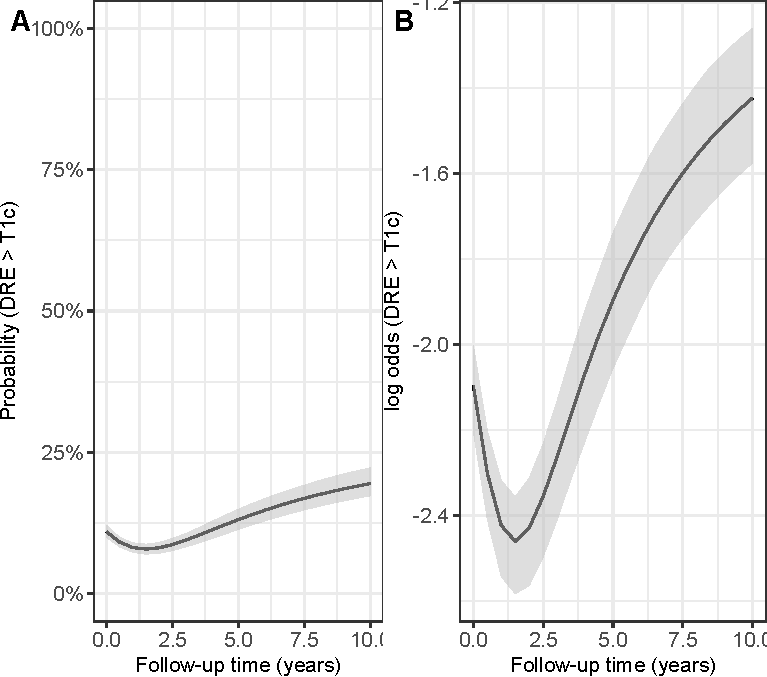
\includegraphics{contents/c3/images/c3_fig_app1.pdf}
\caption{\textbf{Fitted marginal evolution} of the probability of obtaining a DRE larger than T1c, and the corresponding marginal log odds, with 95\% credible interval. These results are for a hypothetical AS patient who is included in AS at the age of 70 years.}
\label{c3:fig:app1}
\end{figure}

\begin{figure}
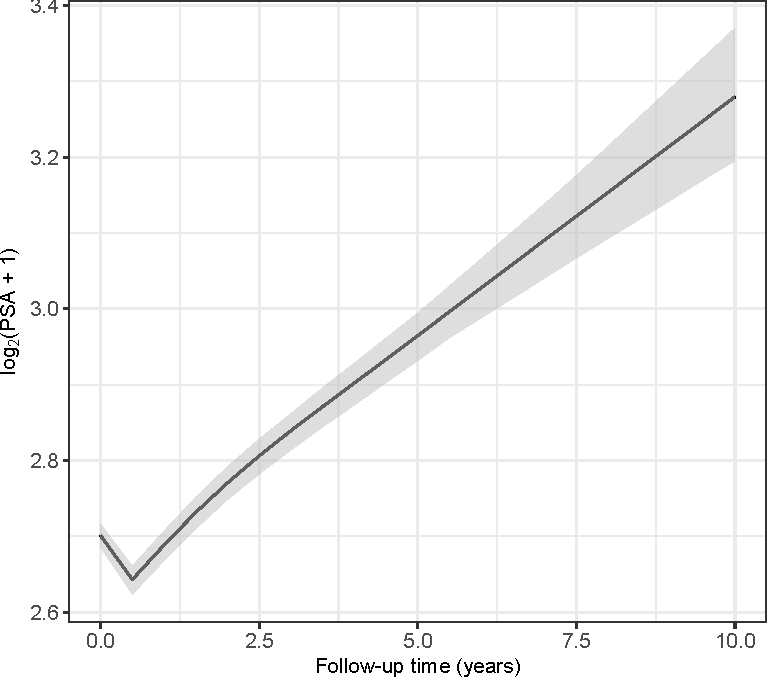
\includegraphics{contents/c3/images/c3_fig_app2.pdf}
\caption{\textbf{Fitted marginal evolution} of $\log_2(\mbox{PSA} + 1)$ measurements over a period of 10 years with 95\% credible interval, for a hypothetical patient who is included in AS at the age of 70 years.}
\label{c3:fig:app2}
\end{figure}

\begin{figure}
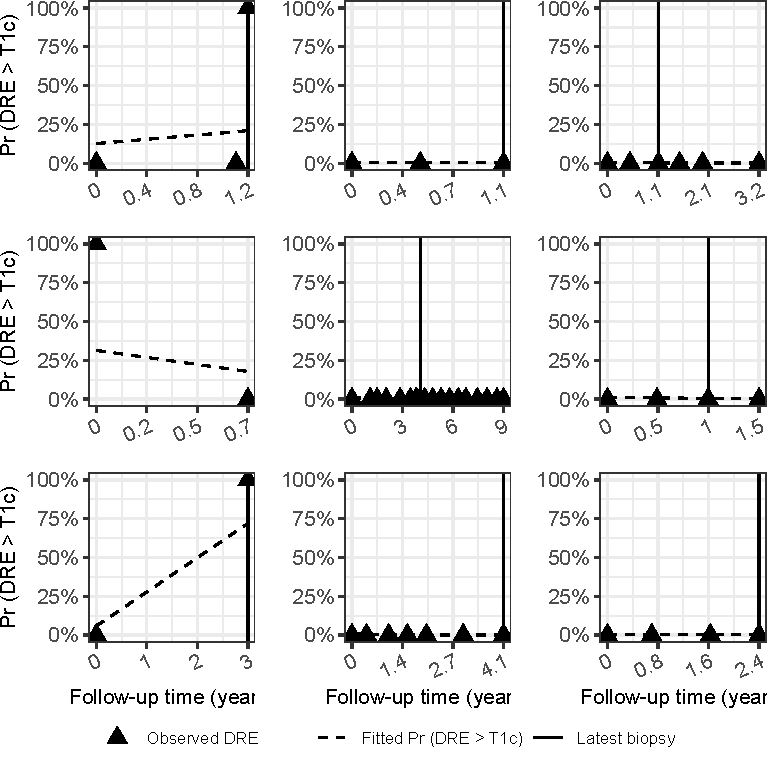
\includegraphics{contents/c3/images/c3_fig_app3.pdf}
\caption{\textbf{Observed DRE versus fitted probabilities} of obtaining a DRE measurement larger than T1c, for nine randomly selected PRIAS patients. The fitted profiles utilize information from the observed DRE measurements, PSA measurements, and time of the latest biopsy. Observed DRE measurements plotted against 0\% probability are equal to T1c. Observed DRE measurements plotted against 100\% probability are larger than T1c.}
\label{c3:fig:app3}
\end{figure}

\begin{figure}
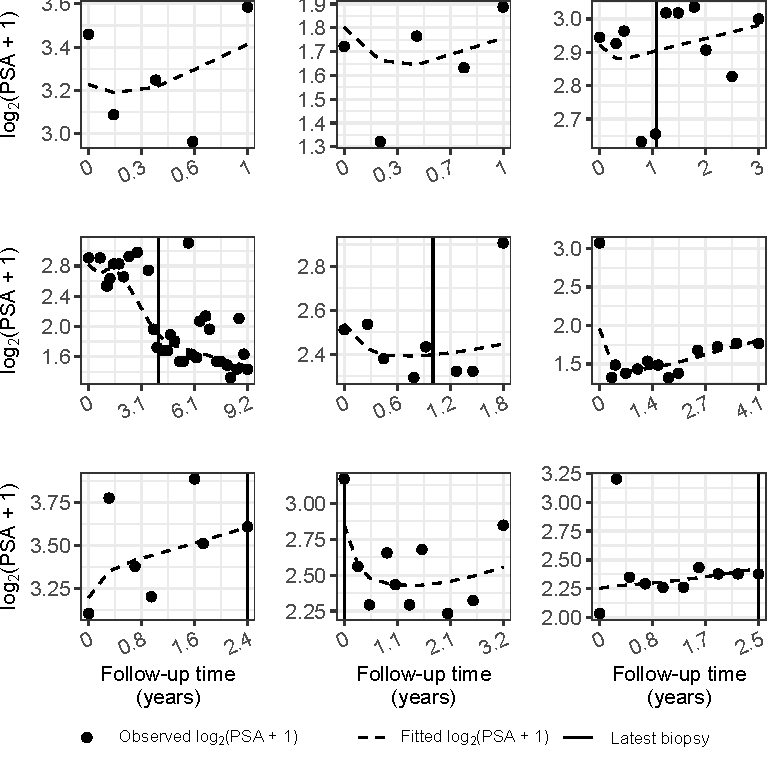
\includegraphics{contents/c3/images/c3_fig_app4.pdf}
\caption{\textbf{Fitted versus observed} ${\log_2(\mbox{PSA} + 1)}$ profiles for nine randomly selected PRIAS patients. The fitted profiles utilize information from the observed PSA measurements, DRE measurements, and time of the latest biopsy.}
\label{c3:fig:app4}
\end{figure}

\begin{figure}
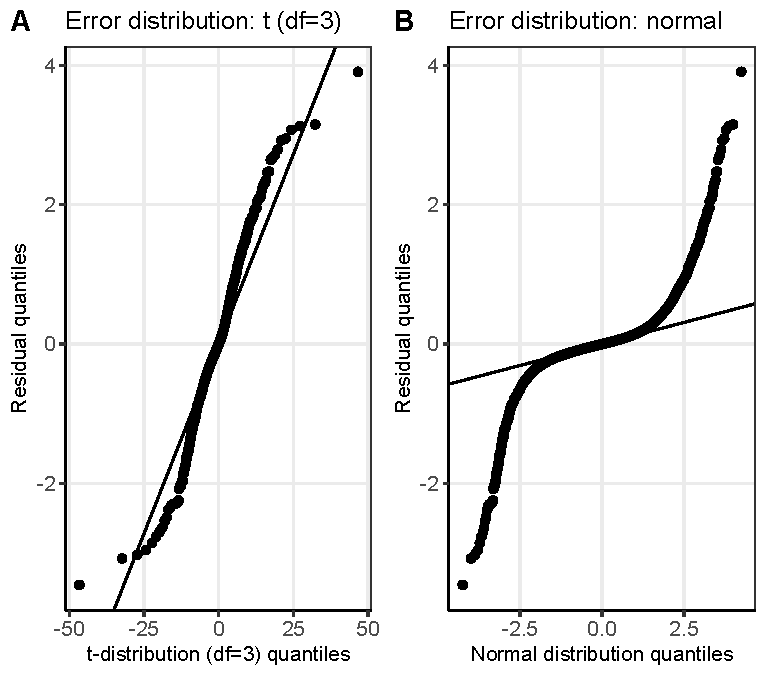
\includegraphics{contents/c3/images/c3_fig_app5.pdf}
\caption{\textbf{Quantile-quantile plot} of the subject-specific residuals from different joint models fitted to the PRIAS dataset. \textbf{Panel A}: model assuming a t-distribution (df=3) for the error term $\varepsilon_p$ \textbf{Panel B}: model assuming a normal distribution for the error term $\varepsilon_p$.}
\label{c3:fig:app5}
\end{figure}

For the relative risk sub-model, the parameter estimates in Table~\ref{c3:table:app1} show that both ${\log_2 (\mbox{PSA} + 1)}$ velocity, and the log odds of having ${\mbox{DRE} > \mbox{T1c}}$ were significantly associated with the hazard of cancer progression. It is important to note that since age, ${\log_2 (\mbox{PSA} + 1)}$ value and velocity, and log odds of ${\mbox{DRE} > \mbox{T1c}}$ are all measured on different scales, a comparison between the corresponding parameter estimates is not easy. To this end, in Table~\ref{c3:table:app2}, we present the hazard (of cancer progression) ratio, for an increase in the aforementioned variables from their first to the third quartile. For example, an increase in log odds of DRE > T1c, from -6.650 to -4.356 (fitted first and third quartiles) corresponds to a hazard ratio of 1.402. The interpretation of the rest is similar.

\begin{table}
\small
\centering
\caption{\textbf{Parameters of the relative-risk sub-model}: Estimated mean and 95\% credible interval. Age is median centered.}
\label{c3:table:app1}
\begin{tabular}{lrrrrr}
\toprule
Variable                      & Mean   & Std. Dev & 2.5\%  & 97.5\%                 & P              \\
\midrule
$(\mbox{Age} - 70)$                      & 0.012    & 0.006 & 0.000 & 0.022  & 0.045 \\
$(\mbox{Age} - 70)^2$ & -0.001   & 0.001 & -0.002 & 0.000      & 0.095 \\
$\mbox{logit} \big\{\mbox{Pr}(\mbox{DRE} > \mbox{T1c})\big\}$                 & 0.147    & 0.017 & 0.115  & 0.183  & \textless0.001     \\
Fitted $\log_2 (\mbox{PSA} + 1)$ value            & 0.104    & 0.078 & -0.044 & 0.256  & 0.193 \\
Fitted $\log_2 (\mbox{PSA} + 1)$ velocity             & 3.396    & 0.564 & 2.376  & 4.475  & \textless0.001   \\
\bottomrule
\end{tabular}
\end{table}

\begin{table}
\small
\centering
\caption{\textbf{Hazard (of cancer progression) ratio and 95\% credible interval (CI)}, for an increase in the variables of relative risk sub-model, from their first quartile ($\mbox{Q}_1$) to their third quartile ($\mbox{Q}_3$). Except for age, quartiles for all other variables are based on their fitted values obtained from the joint model fitted to the PRIAS dataset.}
\label{c3:table:app2}
\begin{tabular}{lrrr}
\toprule
Variable                      & $\mbox{Q}_1$   & $\mbox{Q}_3$ & Hazard ratio [95\% CI] \\
\midrule
Age & 65 & 75 & 1.129 [1.002, 1.251] \\
$\mbox{logit} \big\{\mbox{Pr}(\mbox{DRE} > \mbox{T1c})\big\}$ & -6.650 & -4.356 & 1.402 [1.301, 1.521]\\
$\log_2 (\mbox{PSA} + 1)$ value & 2.336 & 3.053 & 1.079 [0.969, 1.201]\\
$\log_2 (\mbox{PSA} + 1)$ velocity & -0.032 & 0.161 & 1.938 [1.582, 2.372]\\
\bottomrule
\end{tabular}
\end{table}

\subsection{Simulation Study Results}
In the simulation study, we evaluate the following in-practice fixed/heuristic approaches~\citep{loeb2014heterogeneity, inoue2018comparative} for biopsies: biopsy every year, biopsy every one and a half years, biopsy every two years and biopsy every three years. For the personalized biopsy approach, we evaluate three fixed risk thresholds: 5\%, 10\%, and 15\%, and a risk threshold was chosen using $\mbox{F}_1$ score. Lastly, we also evaluate the PRIAS schedule of biopsies. We compare all the aforementioned schedules on two criteria, namely the number of biopsies they schedule and the corresponding delay in detection of cancer progression in years (time of positive biopsy - the true time of cancer progression). The corresponding results, using ${\mbox{500} \times \mbox{250}}$ test patients are presented in Table~\ref{c3:table:app3}.

\begin{table}
\small
\centering
\caption{\textbf{Simulation study results for all patients}: Estimated first, second (median), and third quartiles for number of biopsies ($\mbox{Q}^{\mbox{nb}}_1$, $\mbox{Q}^{\mbox{nb}}_2$, $\mbox{Q}^{\mbox{nb}}_3$) and for the delay in detection of cancer progression ($\mbox{Q}^{\mbox{delay}}_1$, $\mbox{Q}^{\mbox{delay}}_2$, $\mbox{Q}^{\mbox{delay}}_3$), in years, for various biopsy schedules. The delay is equal to the difference between the time of the positive biopsy and the unobserved true time of progression. The results in the table are obtained from test patients of our simulation study.}
\label{c3:table:app3}
\begin{tabular}{l|rrr|rrr}
\toprule
In-practice schedules & $\mbox{Q}^{\mbox{nb}}_1$ & $\mbox{Q}^{\mbox{nb}}_2$ & $\mbox{Q}^{\mbox{nb}}_3$ & $\mbox{Q}^{\mbox{delay}}_1$  & $\mbox{Q}^{\mbox{delay}}_2$  & $\mbox{Q}^{\mbox{delay}}_3$ \\
\midrule
Every year (annual)         & 3  & 10 & 10 & 0.3 & 0.5 & 0.8 \\
Every 1.5 years      & 2  & 7  & 7  & 0.4 & 0.7 & 1.1 \\
Every 2 years       & 2  & 5  & 5  & 0.6 & 1.1 & 1.5 \\
Every 3 years      & 1  & 4  & 4  & 1.1 & 1.8 & 2.3 \\
PRIAS          & 2  & 4  & 6  & 0.3 & 0.7 & 1.0  \\
\midrule
\multicolumn{7}{l}{Personalized approach}\\
\midrule
Risk threshold: 5\%     & 2  & 6  & 8  & 0.3 & 0.6 & 0.9 \\
Risk threshold: 10\%    & 2  & 4  & 5  & 0.3 & 0.7 & 1.0   \\
Risk threshold: 15\%    & 2  & 3  & 4  & 0.4 & 0.8 & 1.4 \\
Risk using $\mbox{F}_1$ score & 1  & 2  & 3  & 0.5 & 0.9 & 2.2 \\
\bottomrule
\end{tabular}
\end{table}


\section{Source Code}
The source code for fitting the joint model is available at \url{https://github.com/anirudhtomer/prias/blob/master/src/chapter3_mdmpaper/fittingModel/jmFit.R}. 

The code generating the simulation population is available at \url{https://github.com/anirudhtomer/prias/blob/master/src/chapter3_mdmpaper/simulationStudy/controller.R}. 

The code for scheduling biopsies using fixed and risk based schedules is available at \url{https://github.com/anirudhtomer/prias/blob/master/src/chapter3_mdmpaper/simulationStudy/schedules.R}.

\end{subappendices}

\clearpage
\bibliographystyle{apalike}
\bibliography{c3_bib}
\chapter[Personalized Schedules for Burdensome Surveillance Tests][Personalized Schedules for Burdensome Surveillance Tests]{Personalized Schedules for Burdensome Surveillance Tests}
\label{c4}

\vspace*{\fill}
\textbf{This chapter is based on the paper}\\
\underline{Tomer, A.}, Nieboer, D., Roobol, M.J., Steyerberg, E.W., and Rizopoulos, D. (2020), Personalized schedules for burdensome surveillance tests. Submitted to \emph{Journal of the American Statistical Association}

\clearpage
\begin{abstract}
Benchmark surveillance \textit{tests} for diagnosing disease \textit{progression} (e.g., biopsies, endoscopies) in early-stage chronic non-communicable diseases (e.g.,~cancer, lung diseases) are usually invasive. For detecting progression timely, patients undergo invasive tests planned in a fixed one-size-fits-all manner (e.g.,~annually). We present personalized test schedules based on progression-risk, that aim to optimize the number of tests (burden) and time delay in detecting progression (shorter is beneficial) better than fixed schedules. Our motivation comes from the problem of scheduling biopsies in prostate cancer surveillance.

Using joint models for time-to-event and longitudinal data, we consolidate patients' longitudinal data (e.g.,~biomarkers) and results of previous tests, into individualized future cumulative-risk of progression. We then create personalized schedules by planning tests on future visits where the predicted cumulative-risk is above a \textit{threshold} (e.g.,~5\% risk). We update personalized schedules with data gathered over follow-up. To find the optimal risk threshold, we minimize a utility function of the expected number of tests (burden) and expected time delay in detecting progression (shorter is beneficial) for different thresholds. We estimate these two in a patient-specific manner for following any schedule, by utilizing a patient's predicted risk profile. Patients/doctors can employ these quantities to compare personalized and fixed schedules objectively.
\end{abstract}
\clearpage
% !TEX root =  ../main_manuscript.tex 
\section{Introduction}
\label{c4:sec:introduction}
Chronic non-communicable diseases (e.g., cancer, lung, cardiovascular diseases) cause 60--70\% of human deaths worldwide~\citep{world2014global}. Often patients diagnosed with an early-stage disease undergo surveillance \emph{tests} to detect disease \emph{progression} timely. A progression is a non-terminal event, and usually a trigger for treatment and/or removal from surveillance. Benchmark tests used for confirming progression are usually \emph{invasive}, e.g., biopsies in prostate cancer surveillance~\citep{bokhorst2015compliance}, endoscopies in Barrett's esophagus~\citep{weusten2017endoscopic}, colonoscopies in colorectal cancer~\citep{krist2007timing}, and bronchoscopies in post lung transplant~\citep{mcwilliams2008surveillance} surveillance.

Invasive tests are repeated until progression is observed, typically as per a one-size-fits-all \emph{fixed schedule}, e.g., biannually,~\citep{krist2007timing,mcwilliams2008surveillance,bokhorst2015compliance}. A time gap between tests causes a time delay in detecting progression (Figure~\ref{c4:fig:1}). A shorter delay in detecting progression (\emph{benefit}) can provide a larger window of opportunity for curative treatment. However, with fixed schedules, this means conducting tests frequently. Frequent tests are \textit{burdensome} as they may cause pain and/or severe medical complications~\citep{krist2007timing,loeb2013systematic}. Consequently, patients may not always comply with frequent tests~\citep{bokhorst2015compliance, LeClercq2015325}. In general, because fixed schedules do not differentiate between fast and slow/non-progressing patients, they impose disproportionate burden/benefits across the patient population.

\begin{figure}
\centerline{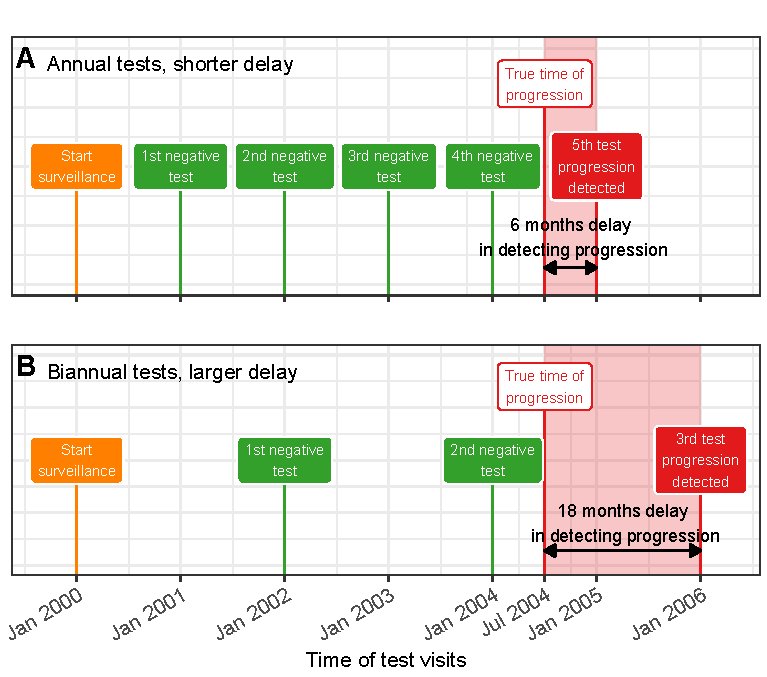
\includegraphics{contents/c4/images/c4_fig1.pdf}}
\caption{\textbf{Goal: Finding the optimal tradeoff between the number of invasive tests (burden) and time delay in detecting progression (shorter is beneficial)}. A progression is a non-terminal event in the surveillance of early-stage chronic non-communicable diseases. The true time of progression for the patient illustrated in this figure is July 2004. Since invasive tests are conducted repeatedly, progression is interval-censored and always observed with a delay. Frequent periodical invasive tests in \textbf{Panel~A} lead to a shorter time delay in detecting progression than infrequent periodical invasive tests in \textbf{Panel~B}. The interval-censored time of progression is Jan~2004--Jan~2005 in \textbf{Panel~A} and between Jan~2004--Jan~2006 in \textbf{Panel~B}.}
\label{c4:fig:1}
\end{figure}

The goal of this work (Figure~\ref{c4:fig:1}) is to optimize the number of invasive tests (burden) and the time delay in detecting progression (shorter is beneficial) better than fixed schedules. Specifically, we intend to \emph{personalize} test schedules using patients' clinical data accumulated over surveillance follow-up. This data includes baseline characteristics, previous test results, and longitudinal outcomes (e.g., biomarkers, medical imaging, physical examination). Many surveillance protocols currently personalize test schedules using heuristic methods such as decision flowcharts~\citep{bokhorst2015compliance,weusten2017endoscopic}. However, flowcharts discretize continuous outcomes, often exploit only the last measurement, ignore the measurement error in observed data, and plan only one test at a time. Alternatively, a complete personalized schedule of tests can be obtained using partially observable Markov decision processes or POMDPs~\citep{alagoz2010operations,steimle2017markov}. Although POMDPs typically discretize continuous longitudinal outcomes to avoid the curse of dimensionality. In scenarios such as ours, where decisions (test/no test) and disease state (low-grade disease/progressed) are both binary, POMDPs may not be necessary either. The reason is that such POMDPs give the same optimal schedule, which can be alternatively obtained by just planning a test when the probability of transition from non-progressed to progressed state is more than a certain threshold~\cite[see][Equation~1]{vickers2006decision}. 

Personalized schedules can also be obtained by optimizing an explicit utility function of the burden and/or benefit of a schedule. A challenge in this approach is quantifying burden and benefit. For a single test decision, \citet{tomer2019personalizedbiometrics} quantify the burden and benefit as the time difference by which the test undershoots (unnecessary test) or overshoots (delayed detection) the true progression time of a patient, respectively. Whereas, for a complete test schedule, \citet{bebu2017optimal} quantify burden as the number of tests planned (or their cost), and benefit as short time delay in detecting progression. Although, unlike the number of tests, the costs of time delay in detecting progression are not always quantifiable. For this issue, \citet{bebu2017optimal}, and \citet{vickers2006decision} have proposed scheduling tests when the risk of progression is above a threshold. Risk-based methodologies has also been explored by \citet{rizopoulos2015personalized}, and to evaluate the choice of risk thresholds \citet{wang2019learning} and \citet{tomer2019personalized} use measures of diagnostic accuracy (e.g., false-positive rate, true positive rate). However, a limitation of risk-based test decisions is that a single decision does not inform patients about the clinical consequences of continuing on surveillance. Also, measures of diagnostic accuracy are not personalized criteria for choosing risk thresholds.

We improve upon the works referenced above in many ways. Instead of a single risk-based test decision, we derive full risk-based test schedules that dynamically update with new clinical data over follow-up. Along with each schedule, we provide patients the clinical consequences of following it. Namely, the expected number of tests that will be required out of all planned tests to detect progression and the expected time delay in detecting progression. Unlike measures of diagnostic accuracy, we calculate these in a personalized manner. Also, these two are easily-quantifiable surrogates for important clinical aspects such as the window of opportunity for curative treatment, risk of adverse outcomes due to delayed detection of progression, financial costs of tests, risk of side-effects, and reduction in quality of life, etc. Our methodology is as follows. We first develop a full specification of the joint distribution of the patient-specific longitudinal outcomes and the time of progression. To this end, we utilize joint models for time-to-event and longitudinal data~\citep{tsiatis2004joint,rizopoulos2012joint} because they are inherently personalized. Specifically, joint models utilize patient-specific random effects~\citep{mcculloch2005generalized} to model longitudinal outcomes without discretizing them. Subsequently, we input clinical data of a new patient into the fitted model to obtain their predicted patient-specific cumulative-risk of progression at future visits. We then create personalized schedules by planning tests on future visits where this predicted cumulative-risk is above a particular \emph{threshold} (e.g., 5\% risk). We automate the choice of this threshold and the resulting schedule. In particular, we optimize a utility function of the expected number of tests (burden) and time delay in detecting progression (shorter is beneficial) for personalized schedules. We estimate these two quantities for any given schedule in a patient-specific manner using the patient's predicted risk profile. Hence, patients/doctors can compare the consequences of opting for personalized versus fixed schedules objectively.

Our motivation comes from the problem of scheduling biopsies in the world's largest prostate cancer surveillance study, called Prostate Cancer Research International Active Surveillance~\citep{bokhorst2015compliance}, or PRIAS. It has 7813 low/very-low grade cancer patients (1134 progressions, 104904 longitudinal measurements), many of whom are potentially over-diagnosed due to prostate-specific antigen (PSA) based screening~\citep{loeb2014overdiagnosis}. To reduce subsequent over-treatment, in surveillance, serious treatments (e.g., surgery, radiotherapy) are delayed until progression is observed. Surveillance involves regular monitoring of a patient's PSA (ng/mL), digital rectal examination or DRE (tumor shape/size), and biopsy Gleason grade group~\citep{epsteinGG2014}. Among these, a biopsy Gleason grade group~$\geq$ 2 is the reference test for confirming progression. Most often, biopsies are scheduled annually~\citep{loeb2014heterogeneity}. However, such a frequent schedule can put an unnecessary burden on patients with slow/non-progressing cancers and cause non-compliance~\citep{bokhorst2015compliance}. Since prostate cancer has the second-highest incidence among all cancers in males~\citep{GlobalCancerStats2012}, individualized biopsy schedules can reduce the burden of biopsies in numerous patients worldwide.

The remaining paper is as follows. Section~\ref{c4:sec:jointmodel} introduces the joint modeling framework. We describe the personalized scheduling methodology in Section~\ref{c4:sec:schedule}, and demonstrate them for prostate cancer surveillance patients in Section~\ref{c4:sec:results}. In Section~\ref{c4:sec:sim_study}, we compare personalized and fixed schedules via a simulation study based on a joint model fitted to the PRIAS dataset.
\section{Joint Model for Time-to-Progression and Longitudinal Outcomes}
\label{c4:sec:jointmodel}
Text currently under embargo.
% !TEX root =  ../main_manuscript.tex 
\section{Personalized Schedule of Invasive Tests for Detecting Progression} 
\label{c4:sec:schedule}

\subsection{Cumulative-risk of progression} 
\label{c4:subsec:cum_risk}
Text currently under embargo.

\subsection{Personalized Test Decision Rule} 
\label{c4:subsec:pers_schedule}
Text currently under embargo.

\subsection{Expected Number of Tests and Expected Time Delay in Detecting Progression}
\label{c4:subsec:exp_delay_estimation}
Text currently under embargo.

\subsection{How to Select the Risk Threshold~$\kappa$}
\label{c4:subsec:kappa_selection}
Text currently under embargo.
\section{Application of Personalized Schedules in Prostate Cancer Surveillance}
\label{c4:sec:results}
We next demonstrate personalized schedules for scheduling biopsies in prostate cancer active surveillance. To this end, we use results from a joint model fitted to the PRIAS dataset introduced in Section~\ref{c4:sec:introduction}. The model definition (Appendix~\ref{c4:appendix:prias_model}) utilized a linear mixed sub-model for biannually measured PSA (continuous: log-transformed from ng/mL), and a logistic mixed sub-model for biannually measured DRE (binary: tumor palpable or not). In the survival sub-model, fitted PSA value, fitted instantaneous PSA velocity (defined in Section~\ref{c4:subsec:surival_sub_model}), and log-odds of having a DRE indicating a palpable tumor, were included as time-dependent predictors. The model parameters were estimated under the Bayesian framework using the R package \textbf{JMbayes}~\citep{rizopoulosJMbayes}, and are presented in Appendix~\ref{c4:appendix:prias_model}. We next briefly present the key results relevant for personalized scheduling.

First, the cause-specific cumulative-risk of cancer progression at the maximum study period of ten years was 50\% (Figure~\ref{c4:fig:app1}). This indicates that many patients may not require all of the yearly biopsies they are usually prescribed. Since personalized schedules are risk-based, their overall performance is dependent on the predictive accuracy and discrimination capacity of the fitted model. In this regard, the model had a moderate time-dependent area under the receiver operating characteristic curve or AUC~\citep{landmarking2017} over the follow-up period (between 0.61 and 0.68). The time-dependent mean absolute prediction error or MAPE~\citep{landmarking2017} was moderate to large (between 0.08 and 0.24) and decreased rapidly after year one of the follow-up. Thus, personalized schedules based on this model may work better after year one with more follow-up data. Details on AUC and MAPE are provided in Appendix~\ref{c5:appendix:validation}.

\subsection{Personalized Biopsy Schedules for a Demonstration Prostate Cancer Patient}
\label{c4:subsec:demo_patient}
We utilized the joint model fitted to the PRIAS dataset to schedule biopsies in a demonstration prostate cancer patient shown in Figure~\ref{c4:fig:5}. The time of his last negative biopsy was $t=3.5$ years, and the time of the current visit was $v=5$ years. We made biopsy decisions over his future visits for PSA measurement $U=\{u_1=5, u_2=5.5,\ldots,u_L=10\}$ years using four different schedules. Two of the fixed schedules are annual biopsy schedule and the PRIAS schedule. The PRIAS schedule has compulsory biopsies at year one, four, seven, and ten of follow-up, and additional annual biopsies if PSA doubling-time~\citep{bokhorst2015compliance} is high. Remaining two schedules are personalized, namely, with a fixed threshold $\kappa=10\%$ risk, and an automatically chosen current visit time $v$ specific risk $\kappa^*(v)$ (Section~\ref{c4:subsec:kappa_selection}). Since the demonstration patient's time of last negative biopsy $t=3.5$ is after year one of follow-up, a time delay in detecting progression
up to three years may not lead to adverse downstream outcomes~\citep{carvalho}.

\begin{figure}
\centerline{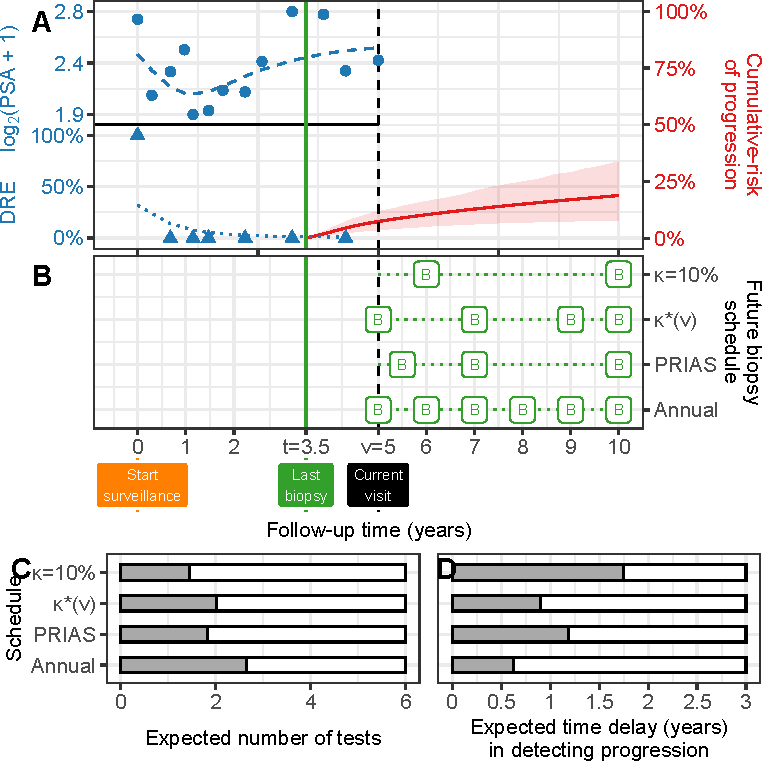
\includegraphics{contents/c4/images/c4_fig5.pdf}}
\caption{\textbf{Personalized schedules for a demonstration prostate cancer patient}. \textbf{Panel~A}: Current visit:~$v=5$ years. Last negative biopsy:~$t=3.5$ years. Longitudinal data:~$\log_2(\mbox{PSA} + 1)$ transformed~\citep{tomer2019personalized} PSA (observed: blue dots, fitted: dashed blue line), binary DRE (observed: blue triangles, fitted probability: dotted blue line). Cumulative-risk profile: solid red line (95\% credible interval shaded). \textbf{Panel~B}: `B' indicates a planned biopsy. \textbf{$\kappa=10\%$} and \textbf{$\kappa^*(v)$} are personalized biopsy schedules using a risk threshold of 10\%, and a visit time~$v$ specific automatic threshold~(\ref{c4:eq:kappa_choice}), respectively. PRIAS biopsy schedule is defined in Section~\ref{c4:subsec:demo_patient}. \textbf{Panel~C,D}: For all schedules we calculate the expected number of tests and expected time delay in detecting progression if the patient progresses before year ten. With a recommended minimum gap of one year between biopsies, maximum possible number of tests are six.}
\label{c4:fig:5}
\end{figure}

The cumulative-risk of progression of the demonstration patient increases 3\% yearly on average, up to 19\% at the maximum study period of ten years. Hence, the patient may progress slowly. Consequently, risk-based personalized approaches plan fewer biopsies than the annual schedule (Panel~B, Figure~\ref{c4:fig:5}). Also, the time delay in detecting progression for personalized schedules (Panel~D, Figure~\ref{c4:fig:5}) is below the safe limit of three years mentioned earlier. Thus, personalized schedules can be a suitable alternative to the annual schedule.
\section{Simulation Study}
\label{c4:sec:sim_study}
Although we evaluated personalized schedules for a demonstration patient, we also intend to analyze and compare personalized and fixed schedules in a full cohort. Our criteria for comparison of schedules are the total number of invasive tests planned (burden), and the actual time delay in detecting progression (shorter is beneficial) for each schedule. Due to the periodical nature of schedules, the actual time delay in detecting progression cannot be observed in real-world surveillance. Hence, instead, we compare personalized versus fixed schedules via an extensive simulated randomized clinical trial in which each hypothetical patient undergoes each schedule. To keep our simulation study realistic, we employ the prostate cancer active surveillance scenario. Specifically, our simulated population is generated using the joint model fitted to the PRIAS cohort (Appendix~\ref{c4:appendix:param_estimates}).

\subsection{Simulation Setup}
From the simulation population, we first sample 500 datasets, each representing a hypothetical prostate cancer surveillance program with 1000 patients in it. We generate a true cancer progression time for each of the ${\mbox{500} \times \mbox{1000}}$ patients, and then sample longitudinal DRE and PSA measurements biannually (PRIAS protocol) for them. We split each dataset into training (750 patients) and test (250 patients) parts, and generate a random and non-informative censoring time for the training patients. All training and test patients also observe Type-I censoring at year ten of follow-up (current study period of PRIAS). We next fit a joint model of the same specification as the model fitted to PRIAS (Appendix~\ref{c4:appendix:param_estimates}), to each of the 500 training datasets and retrieve MCMC samples from the 500 sets of the posterior distribution of the parameters. In each of the 500 hypothetical surveillance programs, we utilize the corresponding fitted joint models to obtain the cumulative-risk of progression in each of the ${\mbox{500} \times \mbox{250}}$ test patients. These cumulative-risk profiles are further used to create personalized biopsy schedules for the test patients. 

For each test patient, we conduct hypothetical biopsies using two fixed (PRIAS and annual schedule) and three personalized biopsy schedules. Personalized schedules are based on, a fixed risk threshold $\kappa=10\%$, an optimal current visit time $v$ specific threshold $\kappa^*(v)$ chosen via~(\ref{c4:eq:kappa_choice}), and an optimal threshold obtained under the constraint that expected time delay in detecting progression is less than 0.75 years (9 months), denoted $\kappa^*\{v \mid E(\mathcal{D})\leq 0.75\}$. The choice of 0.75 years delay constraint is arbitrary and is only used to illustrate that applying the constraint limits the average delay at 0.75 years. Successive personalized biopsy decisions are made only on the standard PSA follow-up visits, utilizing clinical data accumulated only until the corresponding current visit time~(\ref{c4:eq:personalized_decision_grid}). We maintain a minimum recommended gap of one year between consecutive prostate biopsies~\citep{bokhorst2015compliance} as well. Biopsies are conducted until progression is detected, or the maximum follow-up period at year ten (horizon) is reached. The actual time delay in detecting progression is equal to the difference in time at which progression is detected and the actual (simulated) time of progression of a patient.

\subsection{Simulation Results}
In the simulation study, nearly 50\% of the patients observed progression during the ten year study period (\emph{progressing}) and 50\% did not (\emph{non-progressing}). While we can calculate the total number of biopsies scheduled in all $500 \times 250$ test patients, the actual time delay in detecting progression is available only for progressing patients. Hence, we show the simulation results separately for progressing and non-progressing patients (Figure~\ref{c4:fig:6}).

Before discussing delay in detecting progression (Panel~A, Figure~\ref{c4:fig:6}), we note that mean delay up to 1.7 years in all patients~\citep{inoue2018comparative}, and up to three years in patients who progress after year one of follow-up~\citep{carvalho}, may not increase risks of adverse outcomes later. In this regard, the annual biopsies guarantee a maximum delay of one year in all patients. However, they also schedule the highest number of biopsies (Median~3, Inter-quartile range or IQR:~1--6). Much fewer biopsies are planned by the PRIAS schedule (Median~2, IQR:~1--4), but it also has a higher time delay (Median~0.74, IQR: 0.38--1.00 years). The personalized schedule based on optimal risk threshold $\kappa^*(v)$ schedules fewer biopsies than PRIAS and has a delay~(Median~0.86, IQR:~0.46--1.26 years) slightly higher than PRIAS. The expected delay for risk threshold optimized with a constraint on expected delay $\kappa^*\{v \mid E(D)\leq 0.75\}$ is equal to 0.61 years, i.e., the constraint works as expected.

The simulated non-progressing patients (Panel~B,~Figure~\ref{c4:fig:6}) gained the most with personalized schedules. The annual schedule plans 10 (unnecessary) biopsies for each such patient, and the PRIAS schedule plans a median of 6~(IQR:~4--8) biopsies. In contrast, the personalized schedule based on optimized risk threshold $\kappa^*(v)$ plans fewer biopsies consistently (Median~6, IQR:~6--7). The 10\% threshold based schedule plans even fewer biopsies (Median~5, IQR:~4--6).

\begin{figure}
\centerline{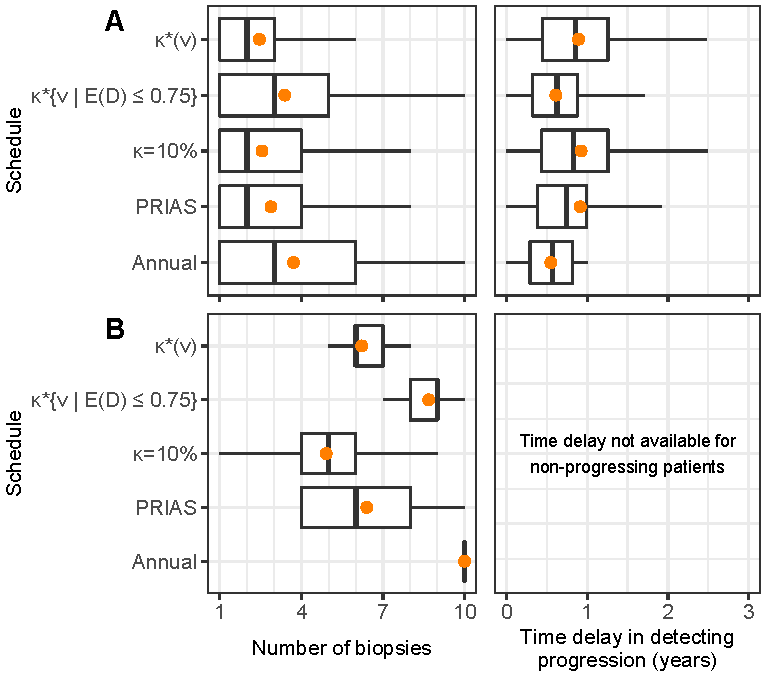
\includegraphics{contents/c4/images/c4_fig6.pdf}}
\caption{\textbf{Number of biopsies and the time delay in detecting cancer progression for various biopsy schedules} obtained via a simulation study. \textbf{Mean} is indicated by the orange circle. Time delay (years) is calculated as (time of positive biopsy - the actual simulated time of cancer progression). Biopsies are conducted until cancer progression is detected. \textbf{Panel~A:} simulated patients who obtained cancer progression in the ten year study period (progressing). \textbf{Panel~B:} simulated patients who did not obtain cancer progression in the ten year study period (non-progressing). Types of schedules: ${\kappa=10\%}$ and $\kappa^*(v)$ schedule a biopsy if the cumulative-risk of cancer progression at the current visit time $v$ is more than 10\%, and an automatically chosen threshold~(\ref{c4:eq:kappa_choice}), respectively. Schedule ${\kappa^*\{v \mid E(\mathcal{D})\leq 0.75\}}$ is similar to $\kappa^*(v)$ except that the euclidean distance in~(\ref{c4:eq:kappa_choice}) is minimized under the constraint that expected delay in detecting progression is at most 9 months (0.75 years). Annual corresponds to a schedule of yearly biopsies, and PRIAS corresponds to biopsies as per PRIAS protocol (Section~\ref{c4:sec:results}).}
\label{c4:fig:6}
\end{figure}
\section{Discussion}
\label{c4:sec:discussion}
Text currently under embargo.

\paragraph{Acknowledgements}
The first and last authors would like to acknowledge support by Nederlandse Organisatie voor Wetenschappelijk Onderzoek (the national research council of the Netherlands) VIDI grant nr. 016.146.301, and Erasmus University Medical Center funding. Part of this work was carried out on the Dutch national e-infrastructure with the support of SURF Cooperative. The authors also thank the Erasmus University Medical Center's Cancer Computational Biology Center for giving access to their IT-infrastructure and software that was used for the computations and data analysis in this study. Last, we would like to thank the PRIAS consortium for enabling this research project.

\section*{Appendix}

\begin{subappendices}
\section{Parameter Estimation}
\label{c4:appendix:param_estimation}
Text currently under embargo.

\section{Joint Model for the PRIAS Dataset Used in Simulation Study}
Text currently under embargo.

\subsection{Model Specification}
Text currently under embargo.

\subsection{Parameter Estimates}
\label{c4:appendix:param_estimates}
Text currently under embargo.

\section{Risk Based Schedules Versus All Possible Schedules}
\label{c4:appendix:all_possible}
Text currently under embargo.

\section{Simulation Study Extended Results}
Text currently under embargo.

\section{Partially Observable Markov Decision Processes}
\label{c4:appendix:pomdp}
Text currently under embargo.

\subsection{Choice of Reward Function for POMDPs}
Text currently under embargo.

\section{Source Code}
\label{c4:appendix:source_code}
Text currently under embargo.

\end{subappendices}

\clearpage
\bibliographystyle{apalike}
\bibliography{c4_bib}
\part{Application}
\chapter[Personalized Biopsy Schedules Based on Risk of Gleason Upgrading for Low-Risk Prostate Cancer Active Surveillance Patients][Upgrading-risk Based Personalized Biopsy Schedules]{Personalized Biopsy Schedules Based on Risk of Gleason Upgrading for Low-Risk Prostate Cancer Active Surveillance Patients}
\label{c5}

\vspace*{\fill}
\textbf{This chapter is based on the paper}\\
\underline{Tomer, A.}, Nieboer, D., Roobol, M.J., Bjartell, A., Steyerberg, E.W., and Rizopoulos, D. (2020), Personalized Biopsy Schedules Based on Risk of Gleason Upgrading for Low-Risk Prostate Cancer Active Surveillance Patients. \emph{BJU International}. Advance online publication. doi:10.1111/bju.15136

\clearpage
% !TEX root =  ../main_manuscript.tex 
\begin{abstract}
\textbf{Objective}: To develop a model and methodology for predicting the risk of Gleason \emph{upgrading} in prostate cancer active surveillance (AS) patients, and using the predicted risks to create risk-based \emph{personalized} biopsy schedules as an alternative to one-size-fits-all schedules (e.g., annually). Furthermore, to assist patients and doctors in making shared decisions of biopsy schedules, by providing them quantitative estimates of the \emph{burden} and \emph{benefit} of opting for personalized versus any other schedule in AS. Last, to externally validate our model and implement it along with personalized schedules in a ready to use web-application.\\

\textbf{Materials and Methods}: Repeat prostate-specific antigen (PSA) measurements, timing and results of previous biopsies, and age at baseline from the world's largest AS study, Prostate Cancer Research International Active Surveillance or PRIAS (7813 patients, 1134 experienced upgrading). We fitted a Bayesian joint model for time-to-event and longitudinal data to this dataset. We then validated our model externally in the largest six AS cohorts of the Movember Foundation's Global Action Plan (GAP3) database (${>20,000}$ patients, 27 centers worldwide). Using the model predicted upgrading-risks, we scheduled biopsies whenever a patient's upgrading-risk was above a certain threshold. To assist patients/doctors in choice of this threshold, and to compare the resulting personalized schedule with currently practiced schedules, along with the timing and the total number of biopsies (burden) planned, for each schedule we provided them the time delay expected in detecting upgrading (shorter is better).\\

\textbf{Results}: The cause-specific cumulative upgrading-risk at year five of follow-up was 35\% in PRIAS, and at most 50\% in GAP3 cohorts. In the PRIAS based model, PSA velocity was a stronger predictor of upgrading (Hazard~Ratio:~2.47, 95\%CI:~1.93--2.99) than PSA value (Hazard~Ratio:~0.99, 95\%CI:~0.89--1.11). Our model had a moderate area under the receiver operating characteristic curve (0.6--0.7) in validation cohorts. The prediction error was moderate (0.1--0.2) in validation cohorts where the impact of PSA value and velocity on upgrading-risk was similar to PRIAS, but large (0.2--0.3) otherwise. Our model required recalibration of baseline upgrading-risk in validation cohorts. We implemented the validated models and the methodology for personalized schedules in a web-application (\url{http://tiny.cc/biopsy}).\\

\textbf{Conclusions}: We successfully developed and validated a model for predicting upgrading-risk, and providing risk-based personalized biopsy decisions, in prostate cancer AS. Personalized prostate biopsies are a novel alternative to fixed one-size-fits-all schedules that may help to reduce unnecessary prostate biopsies while maintaining cancer control. The model and schedules made available via a web-application enable shared decision making of biopsy schedules by comparing fixed and personalized schedules on total biopsies and expected time delay in detecting upgrading.
\end{abstract}
\clearpage
% !TEX root =  ../main_manuscript.tex 
\section{Introduction}
\label{c5:introduction}
Patients with low- and very low-risk screening-detected localized prostate cancer are recommended active surveillance (AS) usually, instead of immediate radical treatment~\citep{briganti2018active}. In AS, cancer progression is monitored routinely via prostate-specific antigen (PSA), digital rectal examination (DRE), repeat biopsies, and recently, magnetic resonance imaging (MRI). Among these, the strongest indicator of cancer-related outcomes is the biopsy Gleason grade group~\citep{epsteinGG2014}. When it increases from group~1 (Gleason 3+3) to 2 (Gleason 3+4) or higher, it is called \emph{upgrading}~\citep{bruinsma2017expert}. Upgrading is an important endpoint in AS upon which patients are commonly advised curative treatment~\citep{bul2013active}.

Biopsies in AS are always conducted with a time gap between them. Consequently, upgrading is always detected with a time delay (Figure~\ref{c5:fig:1}) that cannot be measured directly. In this regard, to detect upgrading timely, many patients are prescribed fixed and frequent biopsies, most often annually~\cite{loeb2014heterogeneity}. However, such one-size-fits-all schedules lead to unnecessary biopsies in slow/non-progressing patients. Biopsies are invasive, may be painful, and are prone to medical complications such as bleeding and septicemia\citep{loeb2013systematic}. Thus, biopsy burden and patient non-compliance to frequent biopsies~\citep{bokhorst2015compliance} have raised concerns regarding the optimal biopsy schedule~\citep{inoue2018comparative, bratt2013study} in AS.

\begin{figure}
\centerline{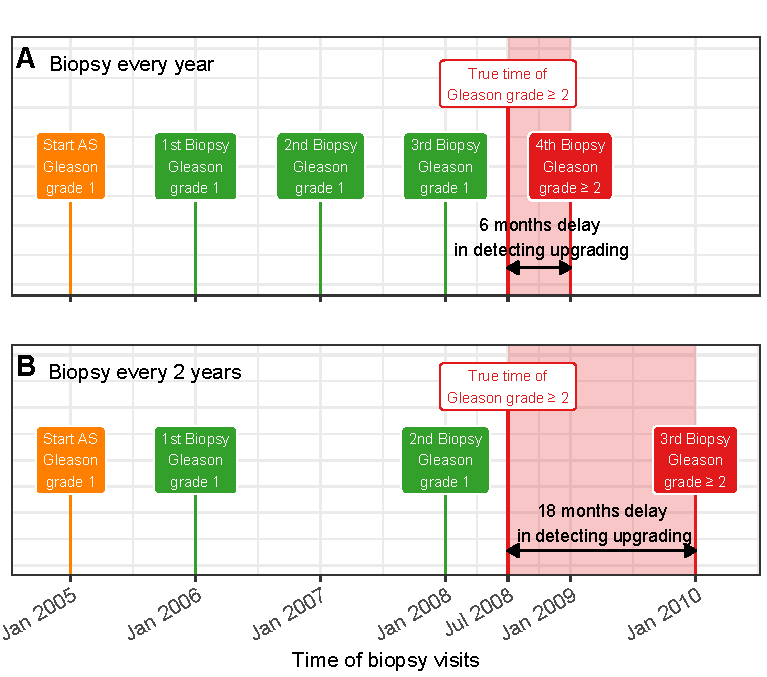
\includegraphics{contents/c5/images/c5_fig1.pdf}}
\caption{\textbf{Trade-off between the timing and number of biopsies (burden) and time delay in detecting Gleason upgrading (shorter is better):} The true time of Gleason upgrading (increase in Gleason grade group from group~1 to~2 or higher) for the patient in this figure is July 2008. When biopsies are scheduled annually (\textbf{Panel~A}), upgrading is detected in January 2009 with a time delay of six months, and a total of four biopsies are scheduled. When biopsies are scheduled biennially (\textbf{Panel~B}), upgrading is detected in January 2010 with a time delay of 18 months, and a total of three biopsies are scheduled. Since biopsies are conducted periodically, the time of upgrading is observed as an interval. For example, between Jan~2008--Jan~2009 in \textbf{Panel~A} and between Jan~2008--Jan~2010 in \textbf{Panel~B}. The phrase `Gleason grade group' is shortened to `Gleason grade' for brevity.}
\label{c5:fig:1}
\end{figure}

Except for the confirmatory biopsy at year one of AS~\citep{bokhorst2015compliance}, opinions and practice regarding the timing of remaining biopsies lack agreement~\citep{nieboer2018active}. Some AS programs utilize patients' observed PSA, DRE, previous biopsy Gleason grade, and lately, MRI results to decide biopsies~\citep{kasivisvanathan2020magnetic,bul2013active,nieboer2018active}. In contrast, others discourage schedules based on clinical data and MRI results~\citep{chesnut2019role,loeb2014heterogeneity}, and instead support periodical one-size-fits-all biopsy schedules. Furthermore, some suggest replacing frequent periodical schedules with infrequent ones (e.g., biennially)~\citep{inoue2018comparative,de2017estimating}. Each of these approaches has limitations. For example, one-size-fits-all schedules can lead to many unnecessary biopsies because of differences in baseline \emph{upgrading-risk} across cohorts~\citep{inoue2018comparative}. Whereas, since observed clinical data has measurement error (e.g., PSA fluctuations), a flaw of using it directly is that it may lead to poor decisions. Also, decisions based on clinical data typically rely only on the latest data point and ignore previous repeated measurements. A novel alternative that counters these drawbacks is first processing patient data via a statistical model, and subsequently using model predicted upgrading-risks to create \emph{personalized} biopsy schedules~\citep{nieboer2018active} (Figure~\ref{c5:fig:2}). While, upgrading-risk calculators are not new~\citep{coley2017prediction,ankerst2015precision,partin1993use,makarov2007updated}, not all are personalized either. Besides, they do not specify how risk predictions can be exploited to create a schedule.

\begin{figure}
\centerline{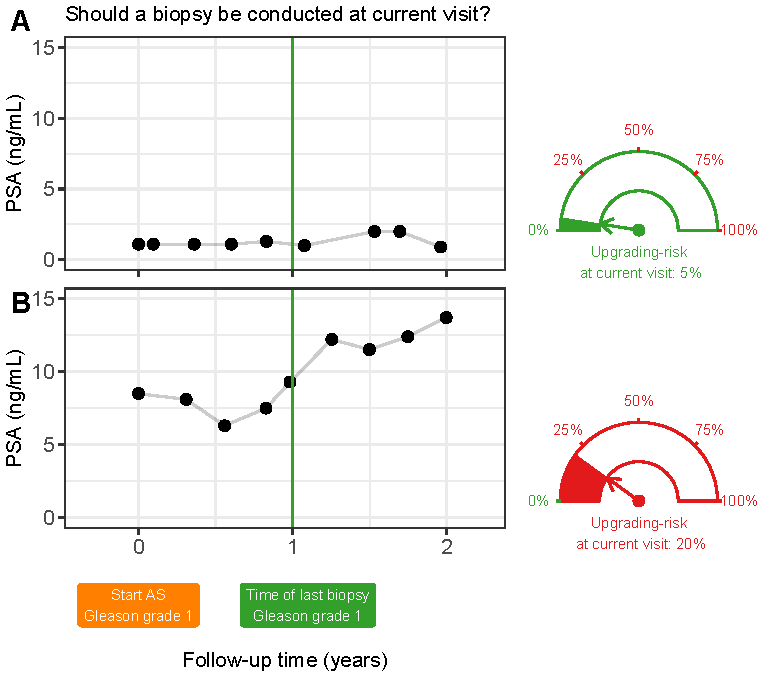
\includegraphics{contents/c5/images/c5_fig2.pdf}}
\caption{\textbf{Motivation for upgrading-risk based personalized biopsy decisions}: To utilize patients' complete longitudinal data and results from previous biopsies in making biopsy decisions. For this purpose, we first process data using a statistical model and then utilize the patient-specific predictions for risk of Gleason upgrading to schedule biopsies. For example, Patient~A (\textbf{Panel~A}) and B (\textbf{Panel~B}) had their latest biopsy at year one of follow-up (green vertical line). Patient~A's prostate-specific antigen (PSA) profile remained stable until his current visit at year two, whereas patient~B's profile has shown a rise. Consequently, patient~B's upgrading-risk at the current visit (year two) is higher than that of patient~A. This makes patient~B a more suitable candidate for biopsy than Patient~A. Risk estimates in this figure are only illustrative.}
\label{c5:fig:2}
\end{figure}

This work is motivated by the problem of scheduling biopsies in AS. We have two goals. First, we want to assist practitioners in using clinical data in biopsy decisions in a statistically sound manner. To this end, we plan to develop a robust, generalizable statistical model that provides reliable individual upgrading-risk in AS. Subsequently, we will employ these predictions to derive risk-based personalized biopsy schedules. Our second goal is to enable shared decision making of biopsy schedules. We intend to achieve this by allowing patients and doctors to compare the \emph{burden} and \emph{benefit} (Figure~\ref{c5:fig:1}) of opting for personalized schedules versus periodical schedules versus schedules based on clinical data. Specifically, we propose timing and number of planned biopsies (more/frequent are burdensome), and the expected time delay in detecting upgrading (shorter is beneficial) for any given schedule. While fulfilling our goals, we want to capture the maximum possible information from the available data. Hence, we will use all repeated measurements of patients, previous biopsy results, baseline characteristics, and keep our model flexible to accommodate future novel biomarkers. To fit this model, we will utilize data of the world's largest AS study, Prostate Cancer Research International Active Surveillance (PRIAS). To evaluate our model, we will externally validate it in the largest six AS cohorts from the Movember Foundation's Global Action Plan (GAP3) database~\citep{gap3_2018}. Last, we aim to implement the validated model and methodology in a web-application.
% !TEX root =  ../main_manuscript.tex 
\section{Patients and Methods}
\label{c5:sec:pat_methods}
\subsection{Study Cohort}
\label{subsec:cohort}
For developing a statistical model to predict upgrading-risk, we used the world's largest AS dataset, Prostate Cancer International Active Surveillance or PRIAS~\citep{bul2013active}, dated April 2019 (Table~\ref{table:prias_summary}). In PRIAS, biopsies were scheduled at year one, four, seven, ten, and additional yearly biopsies were scheduled when PSA doubling time was between zero and ten years. We selected all 7813~patients who had Gleason grade group~1 at inclusion in AS. Our primary event of interest is an increase in this Gleason grade group observed upon repeat biopsy, called \textit{upgrading} (1134~patients). Upgrading is a trigger for treatment advice in PRIAS. Some examples of treatment options in active surveillance are radical prostatectomy, brachytherapy, definitive radiation therapy, and other alternative local treatments such as cryosurgery, High Intensity Focused Ultrasound, and External Beam Radiation Therapy. Comprehensive details on treatment options and their side effects are available in EAU-ESTRO-SIOG guidelines on prostate cancer~\citep{mottet2017eau}. In PRIAS 2250 patients were provided treatment based on their PSA, the number of biopsy cores with cancer, or anxiety/other reasons. However, our reasons for focusing solely on upgrading are that upgrading is strongly associated with cancer-related outcomes, and other treatment triggers vary between cohorts~\citep{nieboer2018active}.

For externally validating our model's predictions, we selected the following largest (by the number of repeated measurements) six cohorts from Movember Foundation's GAP3 database~\citep{gap3_2018} version~3.1, covering nearly 73\% of the GAP3 patients: the University of Toronto AS (Toronto), Johns Hopkins AS (Hopkins), Memorial Sloan Kettering Cancer Center AS (MSKCC), King's College London AS (KCL), Michigan Urological Surgery Improvement Collaborative AS (MUSIC), and University of California San Francisco AS (UCSF, version~3.2). Only patients with a Gleason grade group~1 at the time of inclusion in these cohorts were selected. Summary statistics are presented in Section~\ref{c5:appendix:full_results}.

\begin{table}
\small
\centering
\caption{\textbf{Summary of the PRIAS dataset as of April 2019}. The primary event of interest is upgrading, that is, increase in Gleason grade group from group~1~\citep{epsteinGG2014} to 2 or higher. IQR:~interquartile range, PSA:~prostate-specific antigen. Study protocol URL: \url{https://www.prias-project.org}}
\label{table:prias_summary}
\begin{tabular}{lr}
\toprule
\textbf{Characteristic} & \textbf{Value}\\
\midrule
%Total centers & $> 100$\\
Total patients & 7813\\
Upgrading (primary event) & 1134\\
Treatment & 2250\\
Watchful waiting & 334\\
Loss to follow-up & 249\\
Death (unrelated to prostate cancer) & 95\\
Death (related to prostate cancer) & 2\\
\midrule
Median age at diagnosis (years) & 66 (IQR: 61--71)\\
Median maximum follow-up per patient (years) &  1.8 (IQR: 0.9--4.0)\\
Total PSA measurements & 67578\\
Median number of PSA measurements per patient &  6 (IQR: 4--12)\\
Median PSA value (ng/mL) & 5.7 (IQR: 4.1--7.7)\\
Total biopsies & 15686\\
Median number of biopsies per patient &  2 (IQR: 1--2)\\
\bottomrule
\end{tabular}
\end{table}

\paragraph{Choice of predictors:} In our model, we used all repeated PSA measurements, the timing of the previous biopsy and Gleason grade, and age at inclusion in AS. Other predictors such as prostate volume, MRI results can also be important. MRI is utilized already for targeting biopsies, but regarding its use in deciding the time of biopsies, there are arguments both for and against it~\citep{kasivisvanathan2020magnetic,chesnut2019role,schoots2015magnetic}. MRI is still a recent addition in most AS protocols. Consequently, repeated MRI data is very sparsely available in both PRIAS and GAP3 databases to make a stable prediction model. Prostate volume data is also sparsely available, especially in validation cohorts. Based on these reasons, we did not include them in our model. However, the model we propose next is extendable to include MRI and other novel biomarkers in the future.

% !TEX root =  ../main_manuscript.tex 
\subsection{Statistical Model}
Modeling an AS dataset such as PRIAS, posed certain challenges. First, PSA was measured longitudinally, and over follow-up time it did not always increase linearly. Consequently, we expect that PSA measurements of a patient are more similar to each other than of another patient. In other words, we need to accommodate the within-patient correlation for PSA. Second, PSA was available only until a patient observed upgrading. Thus, we also need to model the association between the Gleason grades and PSA profiles of a patient, and handle missing PSA measurements after a patient experienced upgrading. Third, since the PRIAS biopsy schedule uses PSA, a patient's observed time of upgrading was also dependent on their PSA. Thus, the effect of PSA on the upgrading-risk need to be adjusted for the effect of PSA on the biopsy schedule. Fourth, many patients obtained treatment and watchful waiting before observing upgrading. Since we considered events other than upgrading as censoring, the model needs to account for patients' reasons for treatment or watchful waiting (e.g., age, treatment based on observed data). A model that handles these challenges in a statistically sound manner is the joint model for time-to-event and longitudinal data~\citep{tomer2019,coley2017prediction,rizopoulos2012joint}.

Our joint model consisted of two sub-models. Namely, a linear mixed-effects sub-model~\citep{laird1982random} for longitudinally measured PSA (log-transformed), and a relative-risk sub-model (similar to the Cox model) for the interval-censored time of upgrading. Patient age was used in both sub-models. Results and timing of the previous negative biopsies were used only in the risk sub-model. To account for PSA fluctuations~\citep{nixon1997biological}, we assumed t-distributed PSA measurement errors. The correlation between PSA measurements of the same patient was established using patient-specific random-effects. We fitted a unique curve to the PSA measurements of each patient (Panel~A, Figure~\ref{c5:fig:3}). Subsequently, we calculated the mathematical derivative of the patient's fitted PSA profile~(\ref{c5:eq:rel_risk_model}), to obtain his follow-up time specific instantaneous PSA velocity (Panel~B, Figure~\ref{c5:fig:3}). This instantaneous velocity is a stronger predictor of upgrading than the widely used average PSA velocity~\citep{cooperberg2018refined}. We modeled the impact of PSA on upgrading-risk by employing fitted PSA value and instantaneous velocity as predictors in the risk sub-model (Panel~C, Figure~\ref{c5:fig:3}). We adjusted the effect of PSA on upgrading-risk for the PSA dependent PRIAS biopsy schedule by estimating parameters using a full likelihood method (proof in Chapter~\ref{c2:appendix:B}). This approach also accommodates watchful waiting and treatment protocols that are also based on patient data. Specifically, the parameters (Section~\ref{c5:appendix:model_specification}) of our two sub-models were estimated jointly under the Bayesian paradigm using the R package \textbf{JMbayes}~\citep{rizopoulosJMbayes}.

\begin{figure}
\centerline{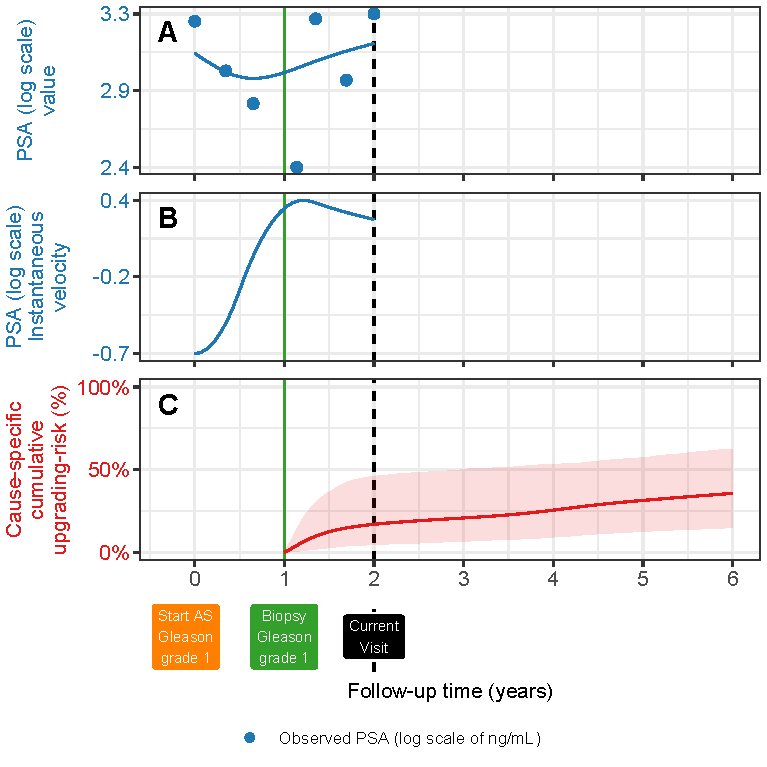
\includegraphics{contents/c5/images/c5_fig3.pdf}}
\caption{\textbf{Illustration of the joint model on a real PRIAS patient}. \textbf{Panel~A:} Observed PSA (blue dots) and fitted PSA (solid blue line), log-transformed from ng/mL. \textbf{Panel~B:} Estimated instantaneous velocity of PSA (log-transformed). \textbf{Panel~C}: Predicted cause-specific cumulative upgrading-risk (95\% credible interval shaded). Upgrading is defined as an increase in the Gleason grade group from group~1~\citep{epsteinGG2014} to 2 or higher. This upgrading-risk is calculated starting from the time of the latest negative biopsy (vertical green line at year one of follow-up). The joint model estimated it by combining the fitted PSA (log scale) value and instantaneous velocity, and time of the latest negative biopsy. Black dashed line at year two denotes the time of current visit.}
\label{c5:fig:3}
\end{figure}

\subsection{Risk Prediction and Model Validation}
Our model provides predictions for upgrading-risk over the entire future follow-up period of a patient (Panel~C, Figure~\ref{c5:fig:3}). However, we recommend using predictions only after year one. This is because most AS programs recommend a confirmatory biopsy at year one, especially to detect patients who may be misdiagnosed as low-grade at inclusion in AS. The model also automatically updates risk-predictions over follow-up as more patient data becomes available (Figure~\ref{c4:fig:2}). We validated our model internally in the PRIAS cohort, and externally in the largest six GAP3 database cohorts. We employed calibration plots~\citep{royston2013external,steyerberg2010assessing} and follow-up \textit{time-dependent} mean absolute risk prediction error or MAPE~\citep{rizopoulos2017dynamic} to graphically and quantitatively evaluate our model's risk prediction accuracy, respectively. We assessed our model's ability to discriminate between patients who experience/do not experience upgrading via the time-dependent area under the receiver operating characteristic curve or AUC~\citep{rizopoulos2017dynamic}. 

The aforementioned \textit{time-dependent} AUC and MAPE~\citep{rizopoulos2017dynamic} are temporal extensions of their standard versions~\citep{steyerberg2010assessing} in a longitudinal setting. Specifically, at every six months of follow-up, we calculated a unique AUC and MAPE for predicting upgrading-risk in the subsequent one year (Appendix~\ref{c5:appendix:validation}). For emulating a realistic situation, we calculated the AUC and MAPE at each follow-up using only the validation data available until that follow-up. Last, to resolve any potential model miscalibration in validation cohorts, we aimed to recalibrate our model's baseline hazard of upgrading (Appendix~\ref{c5:appendix:validation}), individually for each cohort.
% !TEX root =  ../main_manuscript.tex 
\section{Results}
The cause-specific cumulative upgrading-risk at year five of follow-up was 35\% in PRIAS and at most 50\% in validation cohorts (Panel~B, Figure~\ref{c5:fig:4}). In the fitted PRIAS model, the adjusted hazard ratio (aHR) of upgrading for an increase in patient age from 61 to 71 years (25-th to 75-th percentile) was 1.45~(95\%CI:~1.30--1.63). For an increase in fitted PSA value from 2.36 to 3.07 (25-th to 75-th percentile, log scale), the aHR was 0.99~(95\%CI:~0.89--1.11). The strongest predictor of upgrading-risk was instantaneous PSA velocity, with an increase from -0.09 to 0.31 (25-th to 75-th percentile), giving an aHR of 2.47~(95\%CI:~1.93--2.99). The aHR for PSA value and velocity was different in each GAP3 cohort (Table~\ref{c5:tab:PSA_survival_gap3}).

The time-dependent AUC, calibration plot, and time-dependent MAPE of our model are shown in Figure~\ref{c5:fig:4}, and Figure~\ref{c5:fig:auc_pe_recalib}. In all cohorts, time-dependent AUC was moderate (0.6 to 0.7) over the whole follow-up period. Time-dependent MAPE was moderate (0.1 to 0.2) in those cohorts where the impact of PSA on upgrading-risk was similar to PRIAS (e.g., Hopkins cohort, Table~\ref{c5:tab:PSA_survival_gap3}), and large (0.2 to 0.3) otherwise. Our model was miscalibrated for validation cohorts (Panel~B, Figure~\ref{c5:fig:4}), because cohorts had differences in inclusion criteria (e.g., PSA density) and follow-up protocols~\citep{gap3_2018} which were not accounted in our model. Consequently, the PRIAS based model's fitted baseline hazard did not correspond to the baseline hazard in validation cohorts. To solve this problem, we recalibrated the baseline hazard of upgrading in validation cohorts (Figure~\ref{c5:fig:calib_before_after}). We compared risk predictions from the recalibrated models, with predictions from separately fitted cohort-specific joint models (Figure~\ref{c5:fig:calib_in_small}). The difference in predictions was lowest in the Johns Hopkins cohort (impact of PSA on upgrading-risk similar to PRIAS). Comprehensive results are in Appendix~\ref{c5:appendix:full_results} and Appendix~\ref{c5:appendix:validation_res}.

\begin{figure}
\centerline{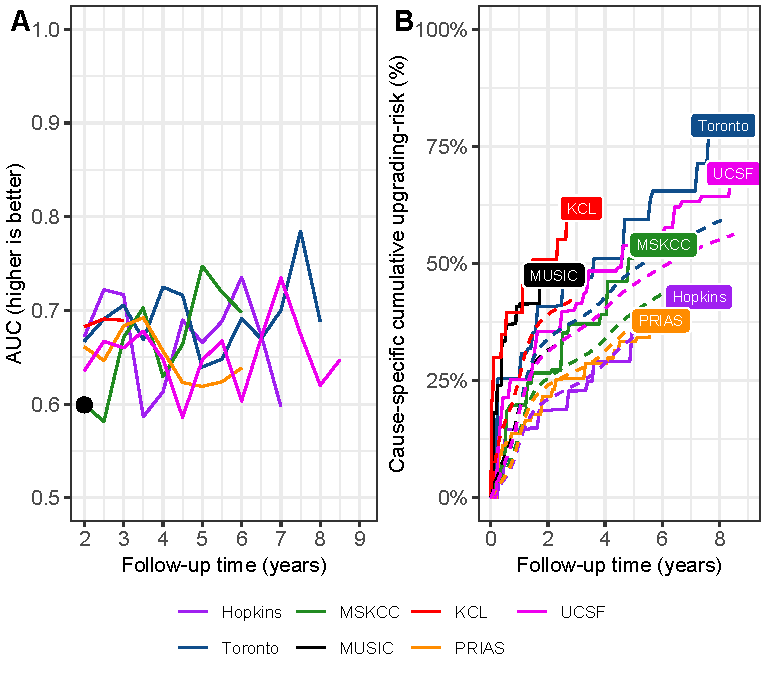
\includegraphics{contents/c5/images/c5_fig4.pdf}}
\caption{\textbf{Model Validation Results}. \textbf{Panel~A}: time-dependent area under the receiver operating characteristic curve or AUC (measure of discrimination). AUC at year one is not shown because we do not intend to replace the confirmatory biopsy at year one. \textbf{Panel~B}: calibration-at-large indicates model miscalibration. This is because solid lines depicting the non-parameteric estimate of the cause-specific cumulative upgrading-risk~\citep{turnbull1976empirical}, and dashed lines showing the average cause-specific cumulative upgrading-risk obtained using the joint model fitted to the PRIAS dataset, are not overlapping. Recalibrating the baseline hazard of upgrading resolved this issue (Figure~\ref{c5:fig:calib_before_after}). Full names of Cohorts are \textit{PRIAS}: Prostate Cancer International Active Surveillance, \textit{Toronto}: University of Toronto Active Surveillance, \textit{Hopkins}: Johns Hopkins Active Surveillance, \textit{MSKCC}: Memorial Sloan Kettering Cancer Center Active Surveillance, \textit{KCL}: King's College London Active Surveillance, \textit{MUSIC}: Michigan Urological Surgery Improvement Collaborative Active Surveillance, \textit{UCSF}: University of California San Francisco AS.}
\label{c5:fig:4}
\end{figure}

\subsection{Personalized Biopsy Schedules}
We employed the PRIAS based fitted model to create personalized biopsy schedules for real PRIAS patients. Particularly, first using the model and patient's observed data, we predicted his cumulative upgrading-risk (Figure~\ref{c5:fig:5}) on all of his future follow-up visits (biannually in PRIAS). Subsequently, we planned biopsies on those future visits where his conditional cumulative upgrading-risk was more than a certain threshold (see Chapter~\ref{c4:sec:schedule} for mathematical details). The choice of this threshold dictates the timing of biopsies in a risk-based personalized schedule. For example, personalized schedules based on 5\% and 10\% risk thresholds are shown in Figure~\ref{c5:fig:5}. 

To facilitate the choice of a risk-threshold, and for comparing the consequences of opting for a risk-based schedule versus any other schedule (e.g., annual, PRIAS), we predict expected time delay in detecting upgrading for following a schedule. We are able to predict this delay for any schedule. For example, in Panel~C of Figure~\ref{c5:fig:5}, the annual schedule has the least expected delay. In contrast, a personalized schedule based on a 10\% risk threshold has a slightly larger expected delay, but it also schedules much fewer biopsies. An important aspect of this delay is that it is personalized as well. That is, even if two different patients are prescribed the same biopsy schedule, their expected delays will be different. This is because delay is estimated using all available clinical data of the patient (Chapter~\ref{c4:subsec:exp_delay_estimation}). While the timing and the total number of planned biopsies denote the burden of a schedule, a shorter expected time delay in detecting upgrading can be a benefit. These two, along with other measures such as a patient's comorbidities, anxiety, etc., can help to make an informed biopsy decision.

\begin{figure}
\centerline{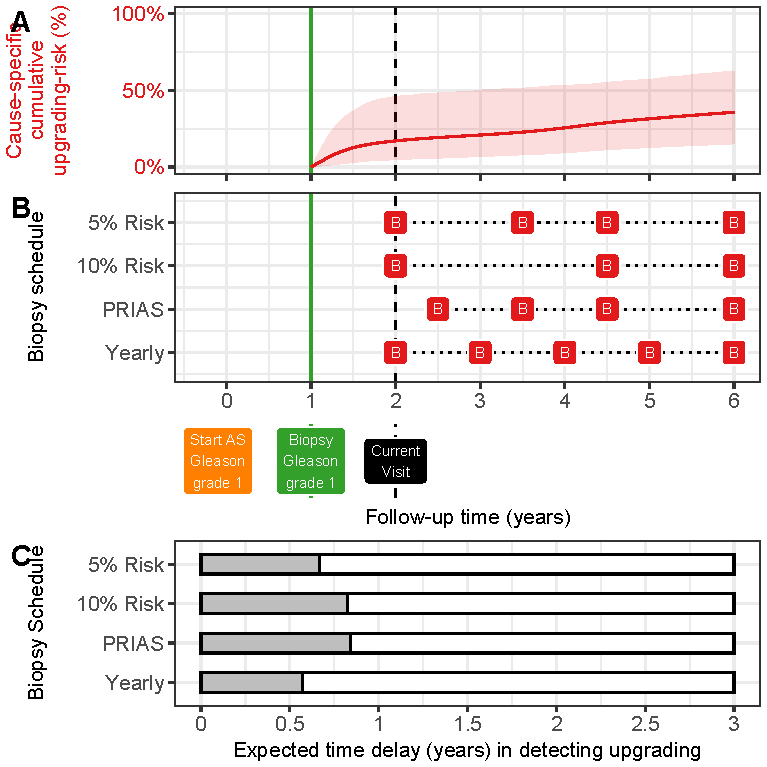
\includegraphics{contents/c5/images/c5_fig5.pdf}}
\caption{\textbf{Illustration of personalized and fixed schedules of biopsies for patient from Figure~\ref{c5:fig:3}}. \textbf{Panel~A:} Predicted cumulative upgrading-risk (95\% credible interval shaded). \textbf{Panel~B:} Different biopsy schedules with a red `B' indicating a future biopsy. Risk:~5\% and Risk:~10\% are personalized schedules in which a biopsy is planned whenever the conditional cause-specific cumulative upgrading-risk is above 5\% or 10\% risk, respectively. Green vertical line at year one is the time of the latest negative biopsy. Black dashed line at year two denotes the time of the current visit. \textbf{Panel~C:} Expected time delay in detecting upgrading (years) if patient progresses before year six. A compulsory biopsy was scheduled at year six (maximum biopsy scheduling time in PRIAS, Table~\ref{c5:tab:max_pred_time}) in all schedules for a meaningful comparison between them.}
\label{c5:fig:5}
\end{figure}

\subsection{Web-Application}
We implemented the PRIAS based model, recalibrated models for GAP3 cohorts, and personalized schedules in a user-friendly web-application \url{https://emcbiostatistics.shinyapps.io/prias_biopsy_recommender/}. This application works on both desktop and mobile devices. Patient data can be entered in Microsoft Excel format. The maximum follow-up time up to which predictions can be obtained depends on each cohort (Table~\ref{c5:tab:max_pred_time}). The web-application supports personalized, annual, and PRIAS schedules. For personalized schedules, users can control the choice of risk-threshold. The web-application also compares the resulting risk-based schedule's timing of biopsies, and expected time delay in detecting upgrading, with annual and PRIAS schedules, to enable sharing biopsy decision making.
% !TEX root =  ../main_manuscript.tex 
\section{Discussion}
We successfully developed and externally validated a statistical model for predicting upgrading-risk~\citep{bruinsma2017expert} in prostate cancer AS, and providing risk-based personalized biopsy decisions. Our work has four novel features over earlier risk calculators~\citep{coley2017prediction,ankerst2015precision}. First, our model was fitted to the world's largest AS dataset PRIAS and externally validated in the largest six cohorts of the Movember Foundation's GAP3 database~\citep{gap3_2018}. Second, the model predicts a patient's current and future upgrading-risk in a personalized manner. Third, using the predicted risks, we created personalized biopsy schedules. We also calculated the expected time delay in detecting upgrading (less is beneficial) for following any schedule. Thus, patients/doctors can compare schedules before making a choice. Fourth, we implemented our methodology in a user-friendly web-application (\url{https://emcbiostatistics.shinyapps.io/prias_biopsy_recommender/}) for both PRIAS and validated cohorts.

Our model and methods can be useful for numerous patients from PRIAS and the validated GAP3 cohorts (nearly 73\% of all GAP3 patients). The model utilizes all repeated PSA measurements, results of previous biopsies, and baseline characteristics of a patient. We could not include MRI and PSA density because of sparsely available data in both PRIAS and GAP3 databases. But, our model is extendable to include them in the near future. The current discrimination ability of our model, exhibited by the \textit{time-dependent} AUC, was between 0.6 and 0.7 over-follow. While this is moderate, it is also so because unlike the standard AUC~\citep{steyerberg2010assessing} the time-dependent AUC is more conservative as it utilizes only the validation data available until the time at which it is calculated. The same holds for the time-dependent MAPE (mean absolute prediction error). Although, MAPE varied much more between cohorts than AUC. In cohorts where the effect size for the impact of PSA value and velocity on upgrading-risk was similar to that for PRIAS (e.g., Hopkins cohort), MAPE was moderate. Otherwise, MAPE was large (e.g., KCL and MUSIC cohorts). We required recalibration of our model's baseline hazard of upgrading for all validation cohorts.

The clinical implications of our work are as follows. First, the cause-specific cumulative upgrading-risk at year five of follow-up was at most 50\% in all cohorts (Panel~B, Figure~\ref{c5:fig:4}). That is, many patients may not require some of the biopsies planned in the first five years of AS. Given the non-compliance and burden of frequent biopsies~\citep{bokhorst2015compliance}, the availability of our methodology as a web-application may encourage patients/doctors to consider upgrading-risk based personalized schedules instead. An additional advantage of personalized schedules is that they update as more patient data becomes available over follow-up. Despite the moderate predictive performance, we expect the overall impact of our model to be positive. There are two reasons for this. First, the risk of adverse outcomes because of the use of personalized schedules is quite low because of the low rate of metastases and prostate cancer specific mortality in AS patients (Table~\ref{table:prias_summary}). Second, studies~\citep{carvalho2017,inoue2018comparative} have suggested that after the confirmatory biopsy at year one of follow-up, biopsies may be done as infrequently as every two to three years, with limited adverse consequences. In other words, longer delays in detecting upgrading may be acceptable after the first negative biopsy. To evaluate the potential harm of personalized schedules, we compared them with fixed schedules in a realistic and extensive simulation study~\citep{tomer2019personalized}. We concluded that personalized schedules plan, on average, six fewer biopsies compared to annual schedule and two fewer biopsies than the PRIAS schedule in slow/non-progressing AS patients, while maintaining almost the same time delay in detecting upgrading as PRIAS schedule. Personalized schedules with different risk thresholds indeed have different performances across cohorts. Thus, to assist patients/doctors in choosing between fixed schedules and personalized schedules based on different risk thresholds, the web-application provides a patient-specific estimate of the expected time delay in detecting upgrading, for both personalized and fixed schedules. We hope that access to these estimates will objectively address patient apprehensions regarding adverse outcomes in AS. Last, we note that our web-application should only be used to decide biopsies after the compulsory confirmatory biopsy at year one of follow-up.

This work has certain limitations. Predictions for upgrading-risk and personalized schedules are available only for a currently limited, cohort-specific, follow-up period (Table~\ref{c5:tab:max_pred_time}). This problem can be mitigated by refitting the model with new follow-up data in the future. Recently, some cohorts started utilizing MRI to explore the possibility of targeting visible lesions by biopsy. Presently, the GAP3 database has limited PSA density and MRI follow-up data available. Since PSA density is used as an entry criterion in some active surveillance studies, including it as a predictor can improve the model. Although, the current model can be extended to include both MRI and PSA density data as predictors when they become available in future. We scheduled biopsies using cause-specific cumulative upgrading-risk, which ignores competing events such as treatment based on the number of positive biopsy cores. Employing a competing-risk model may lead to improved personalized schedules. Upgrading is susceptible to inter-observer variation too. Models which account for this variation~\citep{coley2017prediction,balasubramanian2003estimation} will be interesting to investigate further. Even with an enhanced risk prediction model, the methodology for personalized scheduling and calculation of expected time delay (Chapter~\ref{c4:subsec:exp_delay_estimation}) need not change. Last, our web-application only allows uploading patient data in Microsoft Excel format. Connecting it with patient databases can increase usability.
% !TEX root =  ../main_manuscript.tex 
\section{Conclusions}
We successfully developed a statistical model and methodology for predicting upgrading-risk, and providing risk-based personalized biopsy decisions, in prostate cancer AS. We externally validated our model, covering nearly 73\% patients from the Movember Foundations' GAP3 database. The model made available via a user-friendly web-application (\url{https://emcbiostatistics.shinyapps.io/prias_biopsy_recommender/}) enables shared decision making of biopsy schedules by comparing fixed and personalized schedules on total biopsies and expected time delay in detecting upgrading. Novel biomarkers and MRI data can be added as predictors in the model to improve predictions in the future. Recalibration of baseline upgrading-risk is advised for cohorts not validated in this work.

\paragraph{Acknowledgements}
We thank Jozien Helleman from the Department of Urology, Erasmus University Medical Center, for coordinating the project. The first and last authors would like to acknowledge support by Nederlandse Organisatie voor Wetenschappelijk Onderzoek (the national research council of the Netherlands) VIDI grant nr. 016.146.301, and Erasmus University Medical Center funding. Part of this work was carried out on the Dutch national e-infrastructure with the support of SURF Cooperative. The authors also thank the Erasmus University Medical Center's Cancer Computational Biology Center for giving access to their IT-infrastructure and software that was used for the computations and data analysis in this study. The PRIAS website is funded by the Prostate Cancer Research Foundation, Rotterdam (SWOP). We would like to thank the PRIAS consortium for enabling this research project. 

This work was supported by the Movember Foundation. The funder did not play any role in the study design, collection, analysis or interpretation of data, or in the drafting of this paper.

\paragraph{Conflicts of Interest}
The authors do not report any conflict of interest, and have nothing to disclose.
\section*{Members of The Movember Foundation’s Global Action Plan Prostate Cancer Active Surveillance (GAP3) consortium}

\emph{Principle Investigators:} Bruce Trock (Johns Hopkins University, The James Buchanan Brady Urological Institute, Baltimore, USA), Behfar Ehdaie (Memorial Sloan Kettering Cancer Center, New York, USA), Peter Carroll (University of California San Francisco, San Francisco, USA), Christopher Filson (Emory University School of Medicine, Winship Cancer Institute, Atlanta, USA), Jeri Kim / Christopher Logothetis (MD Anderson Cancer Centre, Houston, USA), Todd Morgan (University of Michigan and Michigan Urological Surgery Improvement Collaborative (MUSIC), Michigan, USA), Laurence Klotz (University of Toronto, Sunnybrook Health Sciences Centre, Toronto, Ontario, Canada), Tom Pickles (University of British Columbia, BC Cancer Agency, Vancouver, Canada), Eric Hyndman (University of Calgary, Southern Alberta Institute of Urology, Calgary, Canada), Caroline Moore (University College London \& University College London Hospital Trust, London, UK), Vincent Gnanapragasam (University of Cambridge \& Cambridge University Hospitals NHS Foundation Trust, Cambridge, UK), Mieke Van Hemelrijck (King's College London, London, UK \& Guy’s and St Thomas’ NHS Foundation Trust, London, UK), Prokar Dasgupta (Guy’s and St Thomas’ NHS Foundation Trust, London, UK), Chris Bangma (Erasmus Medical Center, Rotterdam, The Netherlands/ representative of Prostate cancer Research International Active Surveillance (PRIAS) consortium), Monique Roobol (Erasmus Medical Center, Rotterdam, The Netherlands/ representative of Prostate cancer Research International Active Surveillance (PRIAS) consortium), The PRIAS study group, Arnauld Villers (Lille University Hospital Center, Lille, France), Antti Rannikko (Helsinki University and Helsinki University Hospital, Helsinki, Finland), Riccardo Valdagni (Department of Oncology and Hemato-oncology, Università degli Studi di Milano, Radiation Oncology 1 and Prostate Cancer Program, Fondazione IRCCS Istituto Nazionale dei Tumori, Milan, Italy), Antoinette Perry (University College Dublin, Dublin, Ireland), Jonas Hugosson (Sahlgrenska University Hospital, Göteborg, Sweden), Jose Rubio-Briones (Instituto Valenciano de Oncología, Valencia, Spain), Anders Bjartell (Skåne University Hospital, Malmö, Sweden), Lukas Hefermehl (Kantonsspital Baden, Baden, Switzerland), Lee Lui Shiong (Singapore General Hospital, Singapore, Singapore), Mark Frydenberg (Monash Health; Monash University, Melbourne, Australia), Yoshiyuki Kakehi / Mikio Sugimoto (Kagawa University Faculty of Medicine, Kagawa, Japan), Byung Ha Chung (Gangnam Severance Hospital, Yonsei University Health System, Seoul, Republic of Korea)

\emph{Pathologist:} Theo van der Kwast (Princess Margaret Cancer Centre, Toronto, Canada). 
Technology Research Partners: Henk Obbink (Royal Philips, Eindhoven, the Netherlands), Wim van der Linden (Royal Philips, Eindhoven, the Netherlands), Tim Hulsen (Royal Philips, Eindhoven, the Netherlands), Cees de Jonge (Royal Philips, Eindhoven, the Netherlands).

\emph{Advisory Regional statisticians:} Mike Kattan (Cleveland Clinic, Cleveland, Ohio, USA), Ji Xinge (Cleveland Clinic, Cleveland, Ohio, USA), Kenneth Muir (University of Manchester, Manchester, UK), Artitaya Lophatananon (University of Manchester, Manchester, UK), Michael Fahey (Epworth HealthCare, Melbourne, Australia), Ewout Steyerberg (Erasmus Medical Center, Rotterdam, The Netherlands), Daan Nieboer (Erasmus Medical Center, Rotterdam, The Netherlands); Liying Zhang (University of Toronto, Sunnybrook Health Sciences Centre, Toronto, Ontario, Canada)

\emph{Executive Regional statisticians:} Ewout Steyerberg (Erasmus Medical Center, Rotterdam, The Netherlands), Daan Nieboer (Erasmus Medical Center, Rotterdam, The Netherlands); Kerri Beckmann (King's College London, London, UK \& Guy’s and St Thomas’ NHS Foundation Trust, London, UK), Brian Denton (University of Michigan, Michigan, USA), Andrew Hayen (University of Technology Sydney, Australia), Paul Boutros (Ontario Institute of Cancer Research, Toronto, Ontario, Canada).

\emph{Clinical Research Partners’ IT Experts:} Wei Guo (Johns Hopkins University, The James Buchanan Brady Urological Institute, Baltimore, USA), Nicole Benfante (Memorial Sloan Kettering Cancer Center, New York, USA), Janet Cowan (University of California San Francisco, San Francisco, USA), Dattatraya Patil (Emory University School of Medicine, Winship Cancer Institute, Atlanta, USA), Emily Tolosa (MD Anderson Cancer Centre, Houston, Texas, USA), Tae-Kyung Kim (University of Michigan and Michigan Urological Surgery Improvement Collaborative, Ann Arbor, Michigan, USA), Alexandre Mamedov (University of Toronto, Sunnybrook Health Sciences Centre, Toronto, Ontario, Canada), Vincent LaPointe (University of British Columbia, BC Cancer Agency, Vancouver, Canada), Trafford Crump (University of Calgary, Southern Alberta Institute of Urology, Calgary, Canada), Vasilis Stavrinides (University College London \& University College London Hospital Trust, London, UK), Jenna Kimberly-Duffell (University of Cambridge \& Cambridge University Hospitals NHS Foundation Trust, Cambridge, UK), Aida Santaolalla (King's College London, London, UK \& Guy’s and St Thomas’ NHS Foundation Trust, London, UK), Daan Nieboer (Erasmus Medical Center, Rotterdam, The Netherlands), Jonathan Olivier (Lille University Hospital Center, Lille, France), Tiziana Rancati (Fondazione IRCCS Istituto Nazionale dei Tumori di Milano, Milan, Italy), Helén Ahlgren (Sahlgrenska University Hospital, Göteborg, Sweden), Juanma Mascarós (Instituto Valenciano de Oncología, Valencia, Spain), Annica Löfgren (Skåne University Hospital, Malmö, Sweden), Kurt Lehmann (Kantonsspital Baden, Baden, Switzerland), Catherine Han Lin (Monash University and Epworth HealthCare, Melbourne, Australia), Hiromi Hirama (Kagawa University, Kagawa, Japan), Kwang Suk Lee (Yonsei University College of Medicine, Gangnam Severance Hospital, Seoul, Korea). 

\emph{Research Advisory Committee:} Guido Jenster (Erasmus MC, Rotterdam, the Netherlands), Anssi Auvinen (University of Tampere, Tampere, Finland), Anders Bjartell (Skåne University Hospital, Malmö, Sweden), Masoom Haider (University of Toronto, Toronto, Canada), Kees van Bochove (The Hyve B.V. Utrecht, Utrecht, the Netherlands), Ballentine Carter (Johns Hopkins University, Baltimore, USA – until 2018). 

\emph{Management team:} Sam Gledhill (Movember Foundation, Melbourne, Australia), Mark Buzza / Michelle Kouspou (Movember Foundation, Melbourne, Australia), Chris Bangma (Erasmus Medical Center, Rotterdam, The Netherlands), Monique Roobol (Erasmus Medical Center, Rotterdam, The Netherlands), Sophie Bruinsma / Jozien Helleman (Erasmus Medical Center, Rotterdam, The Netherlands).

\section*{Appendix}
\begin{subappendices}

\section{Model Specification}
\label{c5:appendix:model_specification}
Let $T_i^*$ denote the true time of upgrading (increase in biopsy Gleason grade group from~1 to 2 or higher) for the ${i\mbox{-th}}$ patient included in PRIAS. Since biopsies are conducted periodically, $T_i^*$ is observed with interval censoring ${l_i < T_i^* \leq r_i}$. When upgrading is observed for the patient at his latest biopsy time $r_i$, then $l_i$ denotes the time of the second latest biopsy. Otherwise, $l_i$ denotes the time of the latest biopsy and ${r_i=\infty}$. Let $\boldsymbol{y}_{i}$ denote his observed PSA longitudinal measurements. The observed data of all $n$ patients is denoted by ${\mathcal{A}_n = \{l_i, r_i, \boldsymbol{y}_{i}; i = 1, \ldots, n\}}$.

In our joint model, the patient-specific PSA measurements over time are modeled using a linear mixed effects sub-model. It is given by (see Panel~A, Figure~\ref{c5:fig:3}):
\begin{equation}
\label{c5:eq:long_model_psa}
\begin{split}
    \log_2 \big\{y_{i}(t) + 1\big\} &= m_{i}(t) + \varepsilon_{i}(t),\\
    m_{i}(t) &= \beta_{0} + b_{0i} + \sum_{k=1}^4 (\beta_{k} + b_{ki})  B_k\Big(\frac{t-2}{2},\frac{\mathcal{K}-2}{2}\Big)\\
    & \quad + \beta_{5} \mbox{age}_i,
    \end{split}
\end{equation}
where, $m_{i}(t)$ denotes the measurement error free value of $\log_2 (\mbox{PSA} + 1)$ transformed \citep{pearson1994mixed,lin2000latent} measurements at time $t$. We model it non-linearly over time using B-splines \citep{de1978practical}. To this end, our B-spline basis function ${B_k\{(t-2)/2,(\mathcal{K}-2)/2\}}$ has three internal knots at $\mathcal{K} = \{0.5, 1.3, 3\}$ years, which are the three quartiles of the observed follow-up times. The boundary knots of the spline are at 0 and 6.3 years (95-th percentile of the observed follow-up times). We mean centered (mean 2 years) and standardized (standard deviation 2 years) the follow-up time $t$ and the knots of the B-spline $\mathcal{K}$ during parameter estimation for better convergence. The fixed effect parameters are denoted by ${\{\beta_{0},\ldots,\beta_{5}\}}$, and ${\{b_{0i}, \ldots, b_{4i}\}}$ are the patient specific random effects. The random effects follow a multivariate normal distribution with mean zero and variance-covariance matrix $\boldsymbol{W}$. The error $\varepsilon_{i}(t)$ is assumed to be t-distributed with three degrees of freedom and scale $\sigma$, and is independent of the random effects. 

To model the impact of PSA measurements on the risk of upgrading, our joint model uses a relative risk sub-model. More specifically, the hazard of upgrading denoted as $h_i(t)$, and the cumulative-risk of upgrading denoted as $R_i(t)$, at a time $t$ are (see Panel~C, Figure~\ref{c5:fig:3}):
\begin{equation}
\label{c5:eq:rel_risk_model}
\begin{split}
    h_i(t) &= h_0(t) \exp\Big(\gamma \mbox{age}_i +\alpha_{1} m_{i}(t) + \alpha_{2} \frac{\mathrm{d}m_{i}(t)}{\mathrm{d}{t}}\Big),\\
    R_i(t) &= \exp\Big\{-\int_0^{t} h_i(s)\mathrm{d}{s}\Big\},
    \end{split}
\end{equation}
where, $\gamma$ is the parameter for the effect of age. The impact of PSA on the hazard of upgrading is modeled in two ways, namely the impact of the error free underlying PSA value $m_{i}(t)$ (see Panel~A, Figure~\ref{c5:fig:3}), and the impact of the underlying PSA velocity $\mathrm{d}m_{i}(t)/\mathrm{d}{t}$ (see Panel~B, Figure~\ref{c5:fig:3}). The corresponding parameters are $\alpha_{1}$ and $\alpha_{2}$, respectively. Lastly, $h_0(t)$ is the baseline hazard at time t, and is modeled flexibly using P-splines \citep{eilers1996flexible}. More specifically:
\begin{equation*}
\log{h_0(t)} = \gamma_{h_0,0} + \sum_{q=1}^Q \gamma_{h_0,q} B_q(t, \boldsymbol{v}),
\end{equation*}
where $B_q(t, \boldsymbol{v})$ denotes the $q$-th basis function of a B-spline with knots $\boldsymbol{v} = v_1, \ldots, v_Q$ and vector of spline coefficients $\gamma_{h_0}$. To avoid choosing the number and position of knots in the spline, a relatively high number of knots (e.g., 15 to 20) are chosen and the corresponding B-spline regression coefficients $\gamma_{h_0}$ are penalized using a differences penalty \citep{eilers1996flexible}.

\section{Full Results}
\label{c5:appendix:full_results}
Characteristics of the six validation cohorts from the GAP3 database~\citep{gap3_2018} are shown in Table~\ref{c5:tab:gap3_summary_1}, Table~\ref{c5:tab:gap3_summary_2}, and Table~\ref{c5:tab:gap3_summary_3}. The cause-specific cumulative upgrading-risk in these cohorts is shown in Figure~\ref{c5:fig:app1}.

\begin{figure}
\centerline{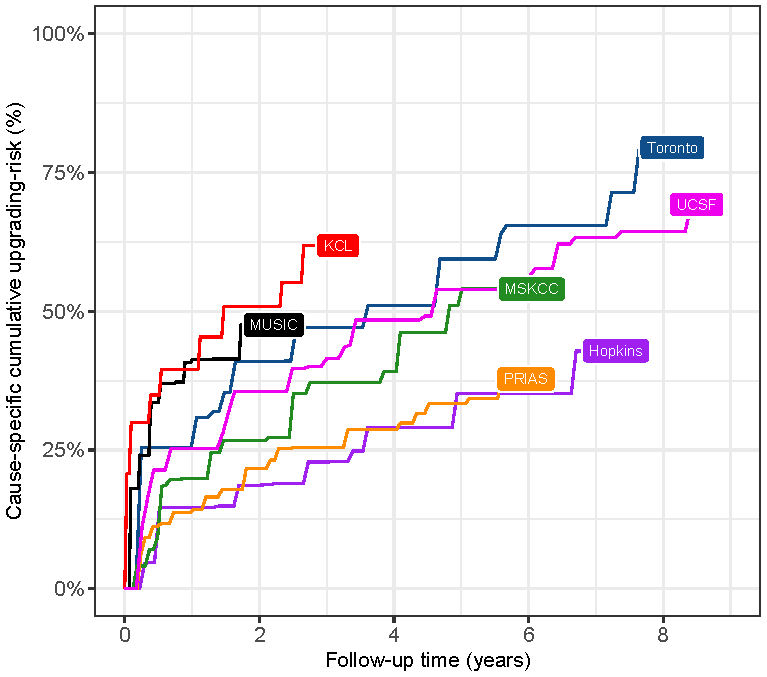
\includegraphics{contents/c5/images/c5_fig_app1.pdf}}
\caption{\textbf{Nonparametric estimate \citep{turnbull1976empirical} of the cause-specific cumulative upgrading-risk} in the world's largest AS cohort PRIAS, and largest six AS cohorts from the GAP3 database \citep{gap3_2018}. Abbreviations are \textit{Hopkins}: Johns Hopkins Active Surveillance, \textit{PRIAS}: Prostate Cancer International Active Surveillance, \textit{Toronto}: University of Toronto Active Surveillance, \textit{MSKCC}: Memorial Sloan Kettering Cancer Center Active Surveillance, \textit{KCL}: King's College London Active Surveillance, \textit{MUSIC}: Michigan Urological Surgery Improvement Collaborative AS, \textit{UCSF}: University of California San Francisco Active Surveillance.}
\label{c5:fig:app1}
\end{figure}

\begin{table}
\small
\centering
\caption{\textbf{Summary of the Hopkins and Toronto validation cohorts from the GAP3 database~\citep{gap3_2018}}. The primary event of interest is upgrading, that is, increase in Gleason grade group from group~1 to 2 or higher. \#PSA: number of PSA, \#biopsies: number of biopsies, IQR:~interquartile range, PSA:~prostate-specific antigen. Full names of cohorts are \textit{Hopkins}: Johns Hopkins Active Surveillance, \textit{Toronto}: University of Toronto Active Surveillance}
\label{c5:tab:gap3_summary_1}
\begin{tabular}{p{5cm}rr}
\hline
\textbf{Characteristic} & \textbf{Hopkins} & \textbf{Toronto}\\
\hline
Total patients & 1392 & 1046\\
Upgrading (primary event) & 260 & 359\\
\hline
Median age (years) & 62 (IQR: 66--69) & 67 (IQR: 60--72)\\
Median maximum follow-up per patient (years) &  3 (IQR: 1.3--5.8) & 4.5 (IQR: 1.9--8.4)\\
Total PSA measurements & 11126 & 13984\\
Median \#PSA per patient &  6 (IQR: 4--11) & 12 (IQR: 7--19)\\
Median PSA (ng/mL) & 4.7 (IQR: 2.9--6.7) & 6 (IQR: 3.7--9.0)\\
Total biopsies & 1926 & 909\\
Median \#biopsies per patient &  1 (IQR: 1--2) &  1 (IQR: 1--2)\\
\hline
\end{tabular}
\end{table}

\begin{table}
\small
\centering
\caption{\textbf{Summary of the MSKCC and UCSF validation cohorts from the GAP3 database~\citep{gap3_2018}}. The primary event of interest is upgrading, that is, increase in Gleason grade group from group~1 to 2 or higher. \#PSA: number of PSA, \#biopsies: number of biopsies, IQR:~interquartile range, PSA:~prostate-specific antigen. Full names of cohorts are \textit{MSKCC}: Memorial Sloan Kettering Cancer Center Active Surveillance, \textit{UCSF}: University of California San Francisco Active Surveillance.}
\label{c5:tab:gap3_summary_2}
\begin{tabular}{p{5cm}rr}
\hline
\textbf{Characteristic} & \textbf{MSKCC} & \textbf{UCSF}\\
\hline
Total patients & 894 & 1397 \\
Upgrading (primary event) & 242 & 547\\
\hline
Median age (years) & 63 (IQR: 57--68) & 63 (IQR: 57--68)\\
Median maximum follow-up per patient (years) & 5.3 (IQR: 1.8--8.3) & 3.6 (IQR: 1.5--7.2)\\
Total PSA measurements & 10704 & 16093\\
Median \#PSA per patient & 11 (IQR: 5--17) & 8 (IQR: 4--16)\\
Median PSA (ng/mL) & 4.7 (IQR: 2.8--7.1) & 5.0 (IQR: 3.4--7.2)\\
Total biopsies & 1102 & 3512\\
Median \#biopsies per patient & 1 (IQR: 1--2) & 2 (IQR: 2--3)\\
\hline
\end{tabular}
\end{table}

\begin{table}
\small
\centering
\caption{\textbf{Summary of the MUSIC and KCL validation cohorts from the GAP3 database~\citep{gap3_2018}}. The primary event of interest is upgrading, that is, increase in Gleason grade group from group~1 to 2 or higher. \#PSA: number of PSA, \#biopsies: number of biopsies, IQR:~interquartile range, PSA:~prostate-specific antigen. Full names of cohorts are \textit{KCL}: King's College London Active Surveillance, \textit{MUSIC}: Michigan Urological Surgery Improvement Collaborative AS.}
\label{c5:tab:gap3_summary_3}
\begin{tabular}{p{5cm}rr}
\hline
\textbf{Characteristic} & \textbf{MUSIC} & \textbf{KCL}\\
\hline
Total patients & 2743 & 616\\
Upgrading (primary event) & 385 & 198\\
\hline
Median age (years) & 65 (IQR: 60--71) & 63 (IQR: 58--68)\\
Median maximum follow-up per patient (years) & 1.2 (IQR: 0.6--2.2) & 2.4 (IQR: 1.3--3.8)\\
Total PSA measurements & 12087 & 2987\\
Median \#PSA per patient & 4 (IQR: 2--6) & 4 (IQR: 2--6)\\
Median PSA (ng/mL) & 5.1 (IQR: 3.4--7.1) & 6 (IQR: 4--9)\\
Total biopsies & 1032 & 484\\
Median \#biopsies per patient & 1 (IQR: 1--1) & 1 (IQR: 1--1)\\
\hline
\end{tabular}
\end{table}

For the relative risk sub-model, the parameter estimates in Table~\ref{c5:tab:PSA_survival} show that ${\log_2 (\mbox{PSA} + 1)}$ velocity and age of the patient were significantly associated with the hazard of upgrading.

\begin{table}
\small
\centering
\caption{\textbf{Parameters of the relative risk sub-model}: Estimated mean and 95\% credible interval for the parameters of the relative-risk sub-model.}
\label{c5:tab:PSA_survival}
\begin{tabular}{lrrrrr}
\hline
Variable                      & Mean   & Std. Dev & 2.5\%  & 97.5\%                 & P              \\
\hline
Age                      & 0.037    & 0.006 & 0.025  & 0.049  & \textless0.001 \\
Fitted $\log_2 (\mbox{PSA} + 1)$ value            & -0.012   & 0.076 & -0.164 & 0.135  & 0.856 \\
Fitted $\log_2 (\mbox{PSA} + 1)$ velocity             & 2.266    & 0.299 & 1.613  & 2.767  & \textless0.001   \\
\hline
\end{tabular}
\end{table}

It is important to note that since age, and ${\log_2 (\mbox{PSA} + 1)}$ value and velocity are all measured on different scales, a comparison between the corresponding parameter estimates is not easy. To this end, in Table \ref{c5:tab:PSA_survival_easy}, we present the hazard ratio of upgrading, for an increase in the aforementioned variables from their 25-th to the 75-th percentile. For example, an increase in fitted $\log_2 (\mbox{PSA} + 1)$ velocity from -0.085 to 0.308 (fitted 25-th and 75-th percentiles) corresponds to a hazard ratio of 2.433. The interpretation of the rest is similar.

\begin{table}
\small
\centering
\caption{\textbf{Hazard ratio and 95\% credible interval (CI) for upgrading}: Variables are on different scale and hence we compare an increase in the variables of relative risk sub-model from their 25-th percentile ($\mbox{P}_{25}$) to their 75-th percentile ($\mbox{P}_{75}$). Except for age, quartiles for all other variables are based on their fitted values obtained from the joint model fitted to the PRIAS dataset.}
\label{c5:tab:PSA_survival_easy}
\begin{tabular}{lrrr}
\hline
Variable                      & $\mbox{P}_{25}$   & $\mbox{P}_{75}$ & Hazard ratio [95\% CI] \\
\hline
Age & 61 & 71 & 1.455 [1.285, 1.631] \\
Fitted $\log_2 (\mbox{PSA} + 1)$ value & 2.360 & 3.078 & 0.991 [0.889, 1.102] \\
Fitted $\log_2 (\mbox{PSA} + 1)$ velocity & -0.085 & 0.308 & 2.433 [1.883, 2.962] \\
\hline
\end{tabular}
\end{table}

\begin{table}
\small
\centering
\caption{\textbf{Parameters of the relative risk sub-model in validation cohorts}. We fitted separate joint models for each of the six GAP3 validation cohorts as well. The specification of these joint models was same as that of the model for PRIAS. Two important predictors in the relative-risk sub-model, namely, the $\log_2 (\mbox{PSA} + 1)$ value and velocity have different impact on upgrading-risk across the cohorts. Table shows the mean estimate of these parameters with 95\% credible interval in brackets. Strongest average effect of $\log_2 (\mbox{PSA} + 1)$ velocity is in PRIAS cohort, whereas the weakest is in MUSIC cohort. The strongest average effect of $\log_2 (\mbox{PSA} + 1)$ value is in the Toronto cohort whereas the weakest is in PRIAS cohort. Full names of cohorts are \textit{Hopkins}: Johns Hopkins Active Surveillance, \textit{PRIAS}: Prostate Cancer International Active Surveillance, \textit{Toronto}: University of Toronto Active Surveillance, \textit{MSKCC}: Memorial Sloan Kettering Cancer Center Active Surveillance, \textit{KCL}: King's College London Active Surveillance, \textit{MUSIC}: Michigan Urological Surgery Improvement Collaborative AS, \textit{UCSF}: University of California San Francisco Active Surveillance.}
\label{c5:tab:PSA_survival_gap3}
\begin{tabular}{lrr}
\hline
Cohort & Fitted $\log_2 (\mbox{PSA} + 1)$ value & Fitted $\log_2 (\mbox{PSA} + 1)$ velocity\\
\hline
PRIAS & -0.012 [-0.164, 0.135] & 2.266 [ 1.613, 2.767]\\
Hopkins & 0.061 [-0.323, 0.329] & 1.839 [ 0.761, 4.378]\\
MSKCC & 0.336 [ 0.081, 0.583] & 1.122 [ 0.421, 1.980]\\
Toronto & 0.572 [ 0.347, 0.794] & 0.943 [ 0.464, 1.554]\\
UCSF & 0.498 [ 0.326, 0.673] & 0.812 [ 0.280, 1.383]\\
MUSIC & 0.441 [ 0.092, 0.767] & 0.029 [-0.552, 0.512]\\
KCL &  0.194 [-0.104, 0.540] & 0.840 [-0.087, 1.665]\\
\hline
\end{tabular}
\end{table}

\section{Risk Predictions for Upgrading}
\label{c5:appendix:validation_res}
Let us assume a new patient $j$, for whom we need to estimate the upgrading-risk. Let his current follow-up visit time be $v$, latest time of biopsy be $t$, observed vector PSA measurements be $\mathcal{Y}_{j}(v)$. The combined information from the observed data about the time of upgrading, is given by the following posterior predictive distribution $g(T^*_j)$ of his time $T^*_j$ of upgrading:
\begin{equation*}
\label{c5:eq:post_pred_dist}
\begin{aligned}
g(T^*_j) &= p\big\{T^*_j \mid T^*_j > t, \mathcal{Y}_{j}(v), \mathcal{A}_n\big\}\\
&= \int \int p\big(T^*_j \mid T^*_j > t, \boldsymbol{b}_j, \boldsymbol{\theta}\big) p\big\{\boldsymbol{b}_j \mid T^*_j>t, \mathcal{Y}_{j}(v), \boldsymbol{\theta}\big\}p\big(\boldsymbol{\theta} \mid \mathcal{A}_n\big) \mathrm{d} \boldsymbol{b}_j \mathrm{d} \boldsymbol{\theta}.
\end{aligned}
\end{equation*}
The distribution $g(T^*_j)$ depends not only depends on the observed data of the patient $T^*_j > t, \mathcal{Y}_{j}(v)$, but also depends on the information from the PRIAS dataset $\mathcal{A}_n$. To this the the posterior distribution of random effects $\boldsymbol{b}_j$ and posterior distribution of the vector of all parameters $\boldsymbol{\theta}$ are utilized, respectively. The distribution $g(T^*_j)$ can be estimated as detailed in \citet{rizopoulos2017dynamic}. Since, many prostate cancer patients may not obtain upgrading in the current follow-up period of PRIAS, $g(T^*_j)$ can only be estimated for a currently limited follow-up period.

The cause-specific cumulative upgrading-risk can be derived from $g(T^*_j)$ as given in~\citep{rizopoulos2017dynamic}. It is given by:
\begin{equation}
\label{c5:eq:dynamic_risk_prob}
R_j(u \mid t, v) = \mbox{Pr}\big\{T^*_j > u \mid T^*_j > t, \mathcal{Y}_{j}(v), \mathcal{A}_n\big\}, \quad u \geq t.
\end{equation}
The personalized risk profile of the patient updates as more data is gathered over follow-up visits. 

\subsection{Validation of Risk Predictions}
\label{c5:appendix:validation}
We wanted to check the usefulness of our model for not only the PRIAS patients but also for patients from other cohorts. To this end, we validated our model in the PRIAS dataset (internal validation) and the largest six cohorts from the GAP3 database~\citep{gap3_2018}. These are the University of Toronto AS (Toronto), Johns Hopkins AS (Hopkins), Memorial Sloan Kettering Cancer Center AS (MSKCC), University of California San Francisco Active Surveillance (UCSF), King's College London AS (KCL), Michigan Urological Surgery Improvement Collaborative AS (MUSIC).

\textbf{\textit{Calibration-in-the-large}}
We first assessed calibration-in-the-large~\citep{steyerberg2010assessing} of our model in the aforementioned cohorts. To this end, we used our model to predict the cause-specific cumulative upgrading-risk for each patient, given their PSA measurements and biopsy results. We then averaged the resulting profiles of cause-specific cumulative upgrading-risk. Subsequently, we compared the averaged cumulative-risk profile with a non-parametric estimate~\citep{turnbull1976empirical} of the cause-specific cumulative upgrading-risk in each of the cohorts. The results are shown in Panel~A of Figure~\ref{c5:fig:calib_before_after}. We can see that our model is miscalibrated in external cohorts, although it is fine in the Hopkins cohort. To improve our model's calibration in all cohorts, we recalibrated the baseline hazard of the joint model fitted to the PRIAS dataset, individually for each of the cohorts except the Hopkins cohort. More specifically, given the data of an external cohort $\mathcal{A}^c$, where $c$ denotes the cohort, the recalibrated parameters $\boldsymbol{\gamma}_{h_0}^c$ (Section~\ref{c5:appendix:model_specification}) of the log baseline hazard are given by:
\begin{equation}
p(\boldsymbol{\gamma}_{h_0}^c \mid \mathcal{A}^c, \boldsymbol{b^c},  \boldsymbol{\theta}) \propto \prod_{i=1}^{n^c} p(l_i^c, r_i^c \mid \boldsymbol{b^c_i}, \boldsymbol{\theta}) p(\boldsymbol{\gamma}_{h_0}^c)
\end{equation}
where $n^c$ are the number of patients in the $c$-th cohort, and $\boldsymbol{\theta}$ is the vector of all parameters of the joint model fitted to the PRIAS dataset. The interval in which upgrading is observed for the $i$-th patient is given by $l_i^c, r_i^c$, with $r_i^c = \infty$ for right-censored patients. The symbol $\boldsymbol{b^c_i}$ denotes patient-specific random effects (Section~\ref{c5:appendix:model_specification}) in the $c$-th cohort. The random effects are obtained using the joint model fitted to the PRIAS dataset before recalibration. We re-evaluated the calibration-in-the-large of our model after the recalibration of the baseline hazard individually for each cohort. The improved calibration-in-the-large is shown in Panel~B of Figure~\ref{c5:fig:calib_before_after}.

\begin{figure}
\centerline{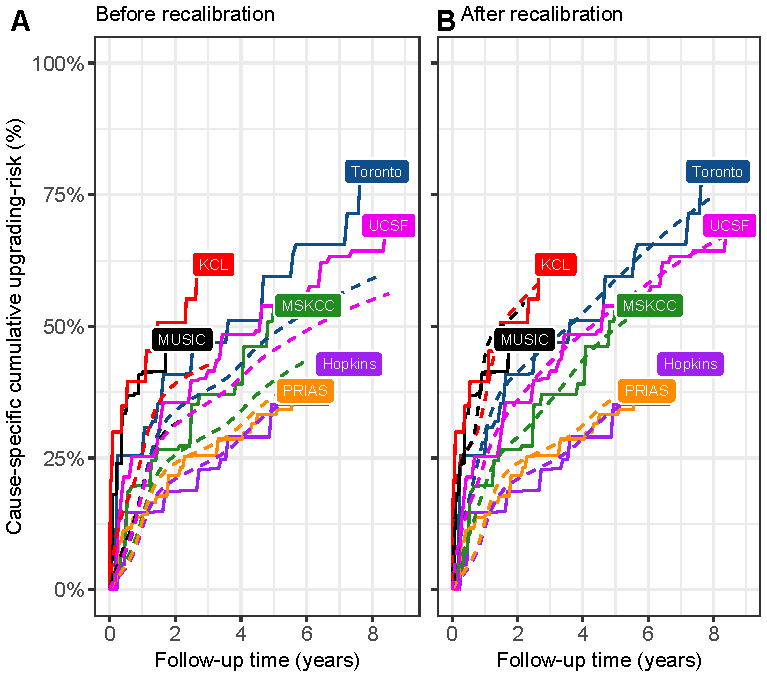
\includegraphics{contents/c5/images/c5_fig_app2.pdf}}
\caption{\textbf{Calibration-in-the-large of our model:}. In \textbf{Panel~A} we can see that our model is not well calibrated for use in KCL, MUSIC, Toronto and MSKCC. In \textbf{Panel~B} we can see that calibration of model predictions improved in KCL, MUSIC, Toronto and MSKCC cohorts after recalibrating our model. Recalibration was not necessary for Hopkins cohort. Full names of Cohorts are \textit{PRIAS}: Prostate Cancer International Active Surveillance, \textit{Toronto}: University of Toronto Active Surveillance, \textit{Hopkins}: Johns Hopkins Active Surveillance, \textit{MSKCC}: Memorial Sloan Kettering Cancer Center Active Surveillance, \textit{KCL}: King's College London Active Surveillance, \textit{MUSIC}: Michigan Urological Surgery Improvement Collaborative Active Surveillance, \textit{UCSF}: University of California San Francisco Active Surveillance.}
\label{c5:fig:calib_before_after}
\end{figure}


\textbf{\textit{Recalibrated PRIAS Model Versus Individual Joint Models For Each Cohort}}
We wanted to check if our recalibrated PRIAS model performed as good as a new joint model that could be fitted to the external cohorts. To this end, we predicted cause-specific cumulative upgrading-risk for each patient from each cohort using two sets of models, namely the recalibrated PRIAS model for each cohort, and a new joint model fitted to each cohort. The difference in predicted cause-specific cumulative upgrading-risk from these models is shown in Figure~\ref{c5:fig:calib_in_small}. We can see that the difference is smaller in those cohorts in which the effects of $\log_2 (\mbox{PSA} + 1)$ value and velocity were similar to that of PRIAS~(Table~\ref{c5:tab:PSA_survival_gap3}). For example, the Hopkins cohort had parameter estimates similar to that of PRIAS, and consequently, the difference in predicted risks for this cohort is smallest. The opposite of this phenomenon holds for the MUSIC and KCL cohorts.
 
\begin{figure}
\centerline{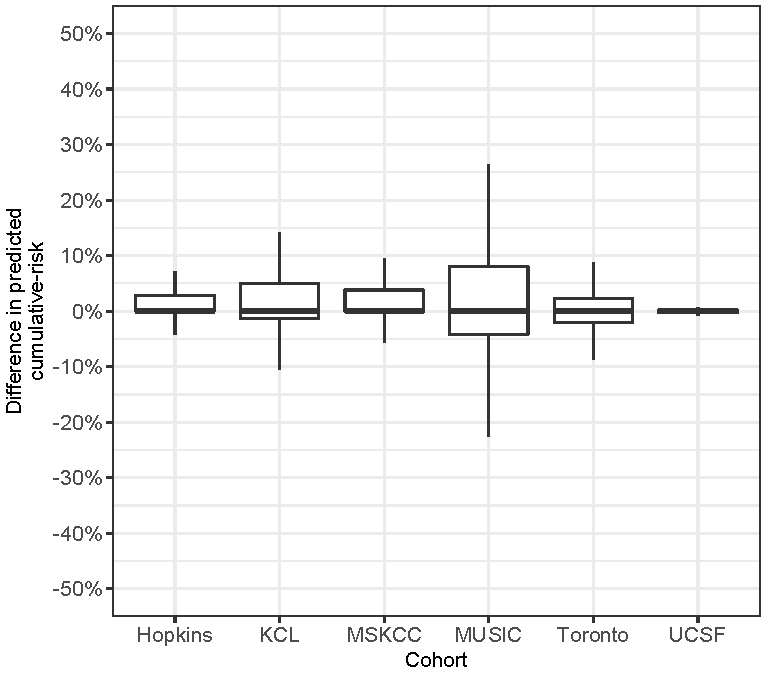
\includegraphics{contents/c5/images/c5_fig_app3.pdf}}
\caption{\textbf{Comparison of predictions from recalibrated PRIAS model with individual joint models fitted to external cohorts:} On Y-axis we show the difference between predicted cause-specific cumulative upgrading-risk for individual patients using two models, namely the recalibrated PRIAS model for each cohort, and individual joint model fitted to each cohort. The figure shows that the difference is smaller in those cohorts in which the effects of $\log_2 (\mbox{PSA} + 1)$ value and velocity were similar to that of PRIAS~(Table~\ref{c5:tab:PSA_survival_gap3}). Full names of Cohorts are \textit{PRIAS}: Prostate Cancer International Active Surveillance, \textit{Toronto}: University of Toronto Active Surveillance, \textit{Hopkins}: Johns Hopkins Active Surveillance, \textit{MSKCC}: Memorial Sloan Kettering Cancer Center Active Surveillance, \textit{KCL}: King's College London Active Surveillance, \textit{MUSIC}: Michigan Urological Surgery Improvement Collaborative Active Surveillance, \textit{UCSF}: University of California San Francisco Active Surveillance.}
\label{c5:fig:calib_in_small}
\end{figure}

\textbf{\textit{Validation of Dynamic Cumulative-Risk Predictions}}
The cumulative-risk predictions from the joint model are dynamic in nature. That is, they update as more data becomes available over time. Consequently, the discrimination and prediction error of the joint model also depend on the available data. We assessed these two measures dynamically in the PRIAS cohort (interval validation) and in the largest six external cohorts that are part of the GAP3 database. For discrimination, we utilized the time-varying area under the receiver operating characteristic curve or time-varying AUC~\citep{rizopoulos2017dynamic}. For time-varying prediction error, we assessed the mean absolute prediction error or MAPE~\citep{rizopoulos2017dynamic}. The AUC indicates how well the model discriminates between patients who experience upgrading, and those do not. The MAPE indicates how accurately the model predicts upgrading. Both AUC and MAPE are restricted to $[0,1]$. However, it is preferred that AUC $>$ 0.5 because an AUC $\leq$ 0.5 indicates that the model performs worse than random discrimination. Ideally, MAPE should be 0.

We calculate AUC and MAPE in a time-dependent manner. More specifically, given the time of latest biopsy $t$, and history of PSA measurements up to time $v$, we calculate AUC and MAPE for a medically relevant time frame $(t, v]$, within which the occurrence of upgrading is of interest. In the case of prostate cancer, at any point in time $v$, it is of interest to identify patients who may have experienced upgrading in the last one year $(v-1, v]$. That is, we set $t=v-1$. We then calculate AUC and MAPE at a gap of every six months (follow-up schedule of PRIAS). That is, $v \epsilon \{1, 1.5, \ldots \}$ years. To obtain reliable estimates of AUC and MAPE, in each cohort, we restrict $v$ to a maximum time point $v_{\mbox{max}}$, such that there are at least ten patients who experience upgrading after $v_{\mbox{max}}$. This maximum time point $v_{\mbox{max}}$ differs between cohorts, and is given in Table~\ref{c5:tab:max_pred_time}.

\begin{table}
\small
\centering
\caption{\textbf{Maximum follow-up period up to which we can reliably predict upgrading-risk and create personalized schedules}. In each cohort, this time point is chosen such that there are at least 10 patients who experience upgrading after this time point. Full names of Cohorts are \textit{PRIAS}: Prostate Cancer International Active Surveillance, \textit{Toronto}: University of Toronto Active Surveillance, \textit{Hopkins}: Johns Hopkins Active Surveillance, \textit{MSKCC}: Memorial Sloan Kettering Cancer Center Active Surveillance, \textit{KCL}: King's College London Active Surveillance, \textit{MUSIC}: Michigan Urological Surgery Improvement Collaborative Active Surveillance, \textit{UCSF}: University of California San Francisco Active Surveillance.}
\label{c5:tab:max_pred_time}
\begin{tabular}{l|r}
\hline
\hline
Cohort & \parbox[t]{3.5cm}{Maximum Prediction\\Time (years)}\\
\hline
PRIAS & 6\\
KCL & 3\\
MUSIC & 2\\
Toronto & 8\\
MSKCC & 6\\
Hopkins & 7\\
UCSF & 8.5\\
\hline
\end{tabular}    
\end{table}

The results for estimates of AUC and MAPE are summarized in Figure~\ref{c5:fig:auc_pe_recalib}, and in Table~\ref{c5:tab:AUC_PE_PRIAS} to Table~\ref{c5:tab:AUC_PE_MUSIC}. Results are based on the recalibrated PRIAS model for the GAP3 cohorts. The results show that AUC remains more or less constant in all cohorts as more data becomes available for patients. The AUC obtains a moderate value, roughly between 0.5 and 0.7 for all cohorts. On the other hand, MAPE reduces by a big margin after year one of follow-up. This could be because of two reasons. Firstly, MAPE at year one is based only on four PSA measurements gathered in the first year of follow-up, whereas after year one number of PSA measurements increases. Secondly, patients in year one consist of two sub-populations, namely patients with a correct Gleason grade group~1 at the time of inclusion in AS, and patients who probably had Gleason grade group~2 at inclusion but were misclassified by the urologist as Gleason grade group~1 patients. To remedy this problem, a biopsy for all patients at year one is commonly recommended in all AS programs~\citep{bokhorst2015compliance}.

\begin{figure}
\centerline{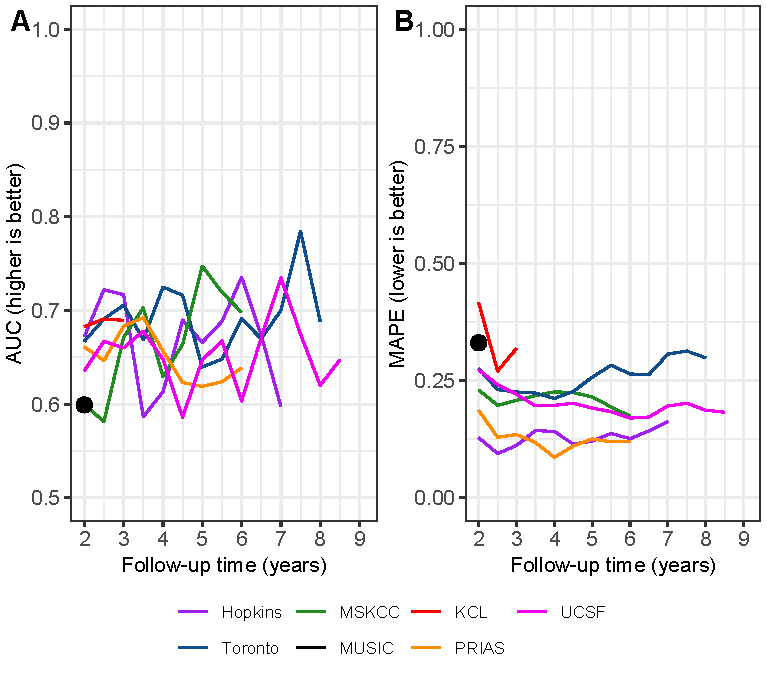
\includegraphics{contents/c5/images/c5_fig_app4.pdf}}
\caption{\textbf{Validation of dynamic predictions of cause-specific cumulative upgrading-risk}. In \textbf{Panel~A} area under the receiver operating characteristic curve or AUC (measure of discrimination) is between 0.6 and 0.7. \textbf{Panel~B} we can see that the time dependent root mean squared prediction error or MAPE is similar for PRIAS and Hopkins cohorts. The bootstrapped 95\% confidence interval for these estimates are presented in Table~\ref{c5:tab:AUC_PE_PRIAS} to Table~\ref{c5:tab:AUC_PE_KCL}. Full names of Cohorts are \textit{PRIAS}: Prostate Cancer International Active Surveillance, \textit{Toronto}: University of Toronto Active Surveillance, \textit{Hopkins}: Johns Hopkins Active Surveillance, \textit{MSKCC}: Memorial Sloan Kettering Cancer Center Active Surveillance, \textit{KCL}: King's College London Active Surveillance, \textit{MUSIC}: Michigan Urological Surgery Improvement Collaborative Active Surveillance, \textit{UCSF}: University of California San Francisco Active Surveillance.}
\label{c5:fig:auc_pe_recalib}
\end{figure}

\begin{table}
\small
\centering
\caption{\textbf{Internal validation of predictions of upgrading in PRIAS cohort}. The area under the receiver operating characteristic curve or AUC (measure of discrimination) and mean absolute prediction error or MAPE are calculated over the follow-up period at a gap of 6 months. In addition bootstrapped 95\% confidence intervals (CI) are also presented.}
\label{c5:tab:AUC_PE_PRIAS}
\begin{tabular}{r|r|r}
\hline
\hline
Follow-up period (years) & AUC (95\% CI) & MAPE (95\%CI)\\ 
\hline
1.0 to 2.0 & 0.661 [0.647, 0.678] & 0.187 [0.183, 0.191]\\
1.5 to 2.5 & 0.647 [0.596, 0.688] & 0.129 [0.122, 0.140]\\
2.0 to 3.0 & 0.683 [0.642, 0.723] & 0.135 [0.125, 0.146]\\
2.5 to 3.5 & 0.692 [0.632, 0.748] & 0.118 [0.111, 0.128]\\
3.0 to 4.0 & 0.657 [0.603, 0.709] & 0.086 [0.080, 0.092]\\
3.5 to 4.5 & 0.623 [0.582, 0.660] & 0.111 [0.105, 0.116]\\
4.0 to 5.0 & 0.619 [0.582, 0.654] & 0.126 [0.118, 0.131]\\
4.5 to 5.5 & 0.624 [0.537, 0.711] & 0.119 [0.103, 0.135]\\
5.0 to 6.0 & 0.639 [0.582, 0.696] & 0.121 [0.103, 0.138]\\
\hline
\end{tabular}    
\end{table}

\begin{table}
\small
\centering
\caption{\textbf{External validation of predictions of upgrading in University of Toronto Active Surveillance cohort}. The area under the receiver operating characteristic curve or AUC (measure of discrimination) and mean absolute prediction error or MAPE are calculated over the follow-up period at a gap of 6 months. In addition bootstrapped 95\% confidence intervals (CI) are also presented.}
\label{c5:tab:AUC_PE_Toronto}
\begin{tabular}{r|r|r}
\hline
\hline
Follow-up period (years) & AUC (95\% CI) & MAPE (95\%CI)\\ 
\hline
1.0 to 2.0 & 0.667 [0.634, 0.712] & 0.276 [0.259, 0.296]\\
1.5 to 2.5 & 0.691 [0.651, 0.730] & 0.231 [0.205, 0.254]\\
2.0 to 3.0 & 0.706 [0.637, 0.762] & 0.226 [0.196, 0.260]\\
2.5 to 3.5 & 0.669 [0.586, 0.741] & 0.224 [0.195, 0.258]\\
3.0 to 4.0 & 0.725 [0.649, 0.806] & 0.212 [0.184, 0.238]\\
3.5 to 4.5 & 0.716 [0.642, 0.793] & 0.227 [0.206, 0.258]\\
4.0 to 5.0 & 0.640 [0.579, 0.717] & 0.257 [0.222, 0.312]\\
4.5 to 5.5 & 0.648 [0.579, 0.740] & 0.283 [0.247, 0.326]\\
5.0 to 6.0 & 0.691 [0.608, 0.793] & 0.264 [0.232, 0.302]\\
5.5 to 6.5 & 0.670 [0.543, 0.776] & 0.263 [0.227, 0.307]\\
6.0 to 7.0 & 0.700 [0.544, 0.851] & 0.307 [0.258, 0.363]\\
6.5 to 7.5 & 0.785 [0.640, 0.866] & 0.313 [0.272, 0.360]\\
7.0 to 8.0 & 0.688 [0.532, 0.786] & 0.299 [0.249, 0.361]\\
\hline
\end{tabular}    
\end{table}

\begin{table}
\small
\centering
\caption{\textbf{External validation of predictions of upgrading in University of California San Francisco Active Surveillance cohort}. The area under the receiver operating characteristic curve or AUC (measure of discrimination) and mean absolute prediction error or MAPE are calculated over the follow-up period at a gap of 6 months. In addition bootstrapped 95\% confidence intervals (CI) are also presented.}
\label{c5:tab:AUC_PE_UCSF}
\begin{tabular}{r|r|r}
\hline
\hline
Follow-up period (years) & AUC (95\% CI) & MAPE (95\%CI)\\ 
\hline
1.0 to 2.0 & 0.635 [0.595, 0.677] & 0.273 [0.266, 0.281]\\
1.5 to 2.5 & 0.667 [0.628, 0.715] & 0.241 [0.224, 0.259]\\
2.0 to 3.0 & 0.660 [0.600, 0.713] & 0.221 [0.205, 0.238]\\
2.5 to 3.5 & 0.678 [0.614, 0.757] & 0.197 [0.175, 0.214]\\
3.0 to 4.0 & 0.648 [0.574, 0.707] & 0.197 [0.179, 0.221]\\
3.5 to 4.5 & 0.586 [0.525, 0.638] & 0.202 [0.180, 0.229]\\
4.0 to 5.0 & 0.647 [0.590, 0.754] & 0.192 [0.168, 0.217]\\
4.5 to 5.5 & 0.667 [0.582, 0.773] & 0.184 [0.159, 0.220]\\
5.0 to 6.0 & 0.603 [0.496, 0.696] & 0.170 [0.144, 0.207]\\
5.5 to 6.5 & 0.671 [0.576, 0.786] & 0.173 [0.145, 0.202]\\
6.0 to 7.0 & 0.735 [0.663, 0.794] & 0.196 [0.166, 0.219]\\
6.5 to 7.5 & 0.675 [0.565, 0.769] & 0.202 [0.168, 0.231]\\
7.0 to 8.0 & 0.620 [0.518, 0.740] & 0.187 [0.144, 0.217]\\
7.5 to 8.5 & 0.647 [0.538, 0.787] & 0.183 [0.146, 0.222]\\
\hline
\end{tabular}    
\end{table}

\begin{table}
\small
\centering
\caption{\textbf{External validation of predictions of upgrading in Johns Hopkins Active Surveillance cohort}. The area under the receiver operating characteristic curve or AUC (measure of discrimination) and mean absolute prediction error or MAPE are calculated over the follow-up period at a gap of 6 months. In addition bootstrapped 95\% confidence intervals (CI) are also presented.}
\label{c5:tab:AUC_PE_Hopkins}
\begin{tabular}{r|r|r}
\hline
\hline
Follow-up period (years) & AUC (95\% CI) & MAPE (95\%CI)\\ 
\hline
1.0 to 2.0 & 0.672 [0.604, 0.744] & 0.128 [0.115, 0.141]\\
1.5 to 2.5 & 0.722 [0.652, 0.792] & 0.095 [0.081, 0.111]\\
2.0 to 3.0 & 0.717 [0.638, 0.777] & 0.112 [0.100, 0.123]\\
2.5 to 3.5 & 0.587 [0.493, 0.704] & 0.144 [0.129, 0.154]\\
3.0 to 4.0 & 0.613 [0.486, 0.742] & 0.141 [0.126, 0.156]\\
3.5 to 4.5 & 0.690 [0.594, 0.783] & 0.115 [0.100, 0.133]\\
4.0 to 5.0 & 0.666 [0.572, 0.754] & 0.121 [0.104, 0.147]\\
4.5 to 5.5 & 0.688 [0.519, 0.779] & 0.137 [0.119, 0.161]\\
5.0 to 6.0 & 0.735 [0.676, 0.820] & 0.126 [0.102, 0.152]\\
5.5 to 6.5 & 0.674 [0.581, 0.765] & 0.143 [0.121, 0.172]\\
6.0 to 7.0 & 0.597 [0.472, 0.712] & 0.163 [0.126, 0.195]\\
\hline
\end{tabular}    
\end{table}

\begin{table}
\small
\centering
\caption{\textbf{External validation of predictions of upgrading in Memorial Sloan Kettering Cancer Center Active Surveillance cohort}. The area under the receiver operating characteristic curve or AUC (measure of discrimination) and mean absolute prediction error or MAPE are calculated over the follow-up period at a gap of 6 months. In addition bootstrapped 95\% confidence intervals (CI) are also presented.}
\label{c5:tab:AUC_PE_MSKCC}
\begin{tabular}{r|r|r}
\hline
\hline
Follow-up period (years) & AUC (95\% CI) & MAPE (95\%CI)\\ 
\hline
1.0 to 2.0 & 0.599 [0.518, 0.671]  & 0.230 [0.207, 0.256]\\
1.5 to 2.5 & 0.581 [0.504, 0.663]  & 0.198 [0.168, 0.235]\\
2.0 to 3.0 & 0.671 [0.599, 0.741]  & 0.208 [0.182, 0.232]\\
2.5 to 3.5 & 0.703 [0.610, 0.777]  & 0.218 [0.197, 0.246]\\
3.0 to 4.0 & 0.629 [0.499, 0.706]  & 0.226 [0.194, 0.259]\\
3.5 to 4.5 & 0.664 [0.589, 0.756]  & 0.225 [0.199, 0.262]\\
4.0 to 5.0 & 0.747 [0.642, 0.841]  & 0.215 [0.188, 0.247]\\
4.5 to 5.5 & 0.719 [0.597, 0.852]  & 0.194 [0.165, 0.232]\\
5.0 to 6.0 & 0.698 [0.565, 0.792]  & 0.174 [0.136, 0.227]\\
\hline
\end{tabular}    
\end{table}

\begin{table}
\small
\centering
\caption{\textbf{External validation of predictions of upgrading in King's College London Active Surveillance cohort}. The area under the receiver operating characteristic curve or AUC (measure of discrimination) and mean absolute prediction error or MAPE are calculated over the follow-up period at a gap of 6 months. In addition bootstrapped 95\% confidence intervals (CI) are also presented.}
\label{c5:tab:AUC_PE_KCL}
\begin{tabular}{r|r|r}
\hline
\hline
Follow-up period (years) & AUC (95\% CI) & MAPE (95\%CI)\\ 
\hline
1.0 to 2.0 & 0.683 [0.604, 0.753] & 0.416 [0.396, 0.445] \\
1.5 to 2.5 & 0.691 [0.621, 0.766] & 0.271 [0.246, 0.297] \\
2.0 to 3.0 & 0.689 [0.616, 0.785] & 0.319 [0.282, 0.344] \\
\hline
\end{tabular}    
\end{table}

\begin{table}
\small
\centering
\caption{\textbf{External validation of predictions of upgrading in Michigan Urological Surgery Improvement Collaborative Active Surveillance cohort}. The area under the receiver operating characteristic curve or AUC (measure of discrimination) and mean absolute prediction error or MAPE are calculated over the follow-up period at a gap of 6 months. In addition bootstrapped 95\% confidence intervals (CI) are also presented.}
\label{c5:tab:AUC_PE_MUSIC}
\begin{tabular}{r|r|r}
\hline
\hline
Follow-up period (years) & AUC (95\% CI) & MAPE (95\%CI)\\ 
\hline
1.0 to 2.0 & 0.599 [0.553, 0.632] & 0.331 [0.317, 0.348]\\
\hline
\end{tabular}    
\end{table}

\section{Source Code}
\label{c5:appendix:source_code}
The R code for fitting the joint model to the PRIAS dataset, is at \url{https://github.com/anirudhtomer/prias/tree/master/src/clinical_gap3}. We refer to this location as `R\_HOME' in the rest of this document. The PRIAS dataset is not openly accessible. However, access to the database can be requested via the contact links at \url{https://www.prias-project.org}.

The PRIAS dataset is in the so-called wide format and also requires the removal of incorrect entries. This can be done via the R script \url{R_HOME/dataset_cleaning.R}. This will lead to two R objects, namely `prias\_final.id' and `prias\_long\_final'. The `prias\_final.id' object contains information about the time of upgrading for PRIAS patients. The `prias\_long\_final' object contains longitudinal PSA measurements, the time of biopsies and results of biopsies.

We use a joint model for time-to-event and longitudinal data to model the evolution of PSA measurements over time, and to simultaneously model their association with the risk of upgrading. The R package we use for this purpose is called \textbf{JMbayes} (https://cran.r-project.org/web/packages/JMbayes/JMbayes.pdf). The API we use, however, is currently not hosted on CRAN, and can be found here:
\url{https://github.com/anirudhtomer/JMbayes}. The joint model can be fitted via the script \url{R_HOME/analysis.R}. It takes roughly 6 hours to run on an Intel Core-i5 machine with four cores and 8GB of RAM. 

The graphs presented in the main manuscript, and the appendix can be generated by the scripts in \url{R_HOME/plots/}.

Validations can be done using the scripts \url{R_HOME/validation/auc_brier/auc_calculator.R}, and \url{R_HOME/validation/auc_brier/gof_calculator.R}. For external validation access to GAP3 database is required.

Once a joint model is fitted to the PRIAS dataset, personalized schedules of biopsies based on the risk of upgrading for new patients can be developed as shown in the script \url{R_HOME/plots/demo_schedule_supplementary.R} or directly using the script \url{https://raw.githubusercontent.com/anirudhtomer/prias/master/src/lastpaper/pers_schedule_api.R}.

Source code for the shiny web application which provides biopsy schedules for patients can be found at \url{R_HOME/shinyapp}
\end{subappendices}

\clearpage
\bibliographystyle{apalike}
\bibliography{c5_bib}
\chapter[Personalized Screening Intervals for Measurement of N-terminal pro-B-type Natriuretic Peptide Improve Efficiency of Prognostication in Patients with Chronic Heart Failure][Personalized Screening Intervals for NT-proBNP]{Personalized Screening Intervals for Measurement of N-terminal pro-B-type Natriuretic Peptide Improve Efficiency of Prognostication in Patients with Chronic Heart Failure}
\label{c6}

\vspace*{\fill}
\textbf{This chapter is an extended version of the paper}\\
Schuurman, A.S., \underline{Tomer, A.}, Akkerhuis, K.M., Brugts, J.J., Constantinescu, A.A., van Ramshorst, J., Umans, V.A., Boersma, E., Rizopoulos, D., and Kardys, I. (2020). Personalized screening intervals for measurement of N-terminal pro-B-type natriuretic peptide improve efficiency of prognostication in patients with chronic heart failure. \emph{European Journal of Preventive Cardiology}. Advance online publication. doi:10.1177/2047487320922639\\

\clearpage
\begin{abstract}
\textbf{Aims.} Personalized screening intervals for N-terminal pro-B-type natriuretic peptide (NT-proBNP) measurement in patients with chronic heart failure (CHF) could maximize information gain on individual patients' disease progression, while minimizing the number of necessary measurements. To improve prevention of clinical adverse events, we compared personalized scheduling of NT-proBNP measurements to fixed scheduling.

\textbf{Methods.} In 263 CHF patients from the Bio-SHiFT study, NT-proBNP was measured trimonthly according to a predefined fixed schedule. The primary endpoint (PE) comprised cardiac death, cardiac transplantation, left ventricular assist device implantation or heart failure hospitalization. We jointly modeled the repeated NT-proBNP measurements and PE. Using this fitted joint model, for each patient at each follow-up visit, we decided the optimal time point of the next NT-proBNP measurement based on the patient's individual NT-proBNP evolution. Personalized scheduling was compared to fixed scheduling by means of a simulation study, based on a replica of the Bio-SHiFT study population. Specifically, we compared the schedules' capability of identification of a high-risk interval (time-window with high risk preceding the PE; identification of its start enables appropriate timely intervention and prevention of PE occurrence), and number of measurements needed.

\textbf{Results.} Compared to fixed scheduling, personalized scheduling saved on average 2 measurements, while the start of the high-risk interval was similar by both approaches [personalized, Median:~6.6, IQR:~4.5-11.3; fixed, Median:~6.3, IQR:~4.2-10.3; months before occurrence of PE]. 

\textbf{Conclusion.} Personalized scheduling of NT-proBNP measurements in CHF patients, as compared to fixed scheduling, shows similar performance with regard to identification of impending adverse events, but requires fewer NT-proBNP measurements.
\end{abstract}
\clearpage
\section{Introduction}
\label{c6:sec:introduction}
Circulating biochemical markers (biomarkers) may reflect the deterioration of patients with chronic heart failure (CHF) in an earlier stage than clinical assessment does. Hence, these biomarkers carry the potential to improve the risk stratification of patients with CHF and prevention of adverse clinical events~\citep{masson2008prognostic,gaggin2013biomarkers}. In the past decade, several trials on natriuretic peptide-guided therapy have been performed in which serial natriuretic peptide measurements were used to titrate medication~\citep{khan2018does,felker2017effect}. However, these trials have demonstrated inconclusive results. This may, in part, be explained by the fact that they mostly used predefined screening intervals (i.e., predefined time points) to assess biomarkers, as well as predefined target levels. Such predefined screening intervals and target levels do not account for individual temporal patterns of biomarkers, which may hamper their potential use for therapy guidance.

Conversely, a personalized screening approach that individualizes screening intervals and target levels based on individual temporal biomarker patterns may further improve risk assessment and therapy guidance. Such personalized screening intervals aim to maximize information gain on the individual patients' disease progression, while minimizing the necessary number of measurements, and therewith costs and patient burden~\citep{rizopoulos2016personalized}. In order to establish such intervals and targets, a model should be applied that incorporates detailed data on individual temporal patterns. Joint modeling is a statistical approach that takes into account full individual temporal patterns of biomarkers and links these patterns to the occurrence of adverse clinical events~\citep{rizopoulosJMbayes,rizopoulos2014tools}. In the Role of Biomarkers and Echocardiography in Prediction of Prognosis of Chronic Heart Failure Patients (Bio-SHiFT) study, we collected a median of 9 [interquartile range (IQR):~5--10] blood samples per patient. We demonstrated, by applying joint modeling, that individual temporal patterns of serially measured CHF-related biomarkers are associated with the prognosis of CHF patients~\citep{van2018toward}. Furthermore, we demonstrated that such a joint model when fitted on patients in Bio-SHiFT, could be used to estimate the patient-specific risk of the adverse outcome at each visit at the outpatient clinic. This risk is updated at each visit because it incorporates information on the patients' prognosis as derived from the newly available biomarker measurement~\citep{van2018toward}.

Subsequently, such a patient-specific risk profile, as derived from a joint model, can be applied to establish personalized screening intervals for future patients presenting at the outpatient clinic. This approach could contribute to improved prevention of further adverse clinical events. However, the benefits of this approach, over predefined screening intervals and targets, have not yet been investigated in CHF. Thus, in the current investigation, we aim to compare personalized scheduling to predefined fixed scheduling of N-terminal pro-B-type natriuretic peptide (NT-proBNP) measurements in individual CHF patients, in terms of the number of measurements performed according to each schedule, as well as the amount of time that remains for intervention before adverse outcome occurs. For this purpose, we use the data of the Bio-SHiFT study.
\section{Methods}
\label{c6:sec:methods}

\subsection{Study design and procedures}
The design of the Bio-SHiFT study has been described in detail elsewhere~\citep{van2018toward}. Briefly, CHF patients in clinically stable conditions were recruited during their regular outpatient visits in the Erasmus MC, Rotterdam, The Netherlands, and Northwest Clinics, Alkmaar, The Netherlands. Patients were eligible if CHF (with reduced or preserved ejection fraction) was diagnosed $\geq$~3 months ago according to the guidelines of the European Society of Cardiology~\citep{mcmurray2012v,paulus2007diagnose,dickstein2008stro}. Blood samples were taken on the day of inclusion and at predefined trimonthly follow-up visits, which were scheduled to a maximum follow-up duration of 30 months. Blood sampling and study procedures are further described in the Supplemental Materials. For the current investigation, we used 263 patients who were enrolled during the first inclusion period between October 2011 and June 2013. 

During follow-up, the occurrence of clinical events was recorded in the electronic case report forms, and associated hospital records and discharge letters were collected. Subsequently, a clinical event committee, blinded to the biomarker-candidate results, reviewed hospital records and discharge letters, and adjudicated the study endpoints. The primary study endpoint (PE) was defined as the composite of cardiac death, cardiac transplantation, left ventricular assist device implantation, or hospitalization for heart failure, whichever occurred first.

The Bio-SHiFT study was approved by the medical ethics committee of the Erasmus MC and was performed in accordance with the Declaration of Helsinki. Written informed consent was obtained from all patients. The Bio-SHiFT study is registered in ClinicalTrials.gov, number NCT01851538.

\subsection{Statistical analysis}
We utilized a joint model to estimate the association between longitudinally measured NT-proBNP and clinical outcome~\citep{rizopoulos2012joint,tsiatis2004joint}. A joint model combines a linear mixed-effect (LME) model for longitudinally measured data with a Cox regression model for time-to-event data. The association between these two types of data is modeled using patient-specific random effects. The LME model uses these random-effects to model the longitudinal temporal pattern of NT-proBNP measurements. The Cox model uses these random-effects to model the impact of the underlying trajectory of NT-proBNP measurements on the risk of PE~\citep{rizopoulos2016personalized,van2018toward}. The use of joint modeling is further motivated in Supplemental Materials. We used logarithmically (base 2) transformed NT-proBNP measurements in our joint model. Consequently, we were able to obtain a hazard ratio (HR) along with a 95\% confidence interval (CI) that estimated the risk of the PE associated with doubling of NT-proBNP level at a given follow-up time~\citep{van2018toward}.

The potential confounders that we used in our joint model were chosen based on their independent association with the PE in multivariable Cox regression models (NYHA class and diabetes mellitus) and existing literature (age, gender, renal function, body mass index). Covariates were missing in less than 3\% of the patients. Multiple imputations (5 times) of these covariates were performed in the multivariable analyses. 

\subsection{Scheduling personalized screening visits}
The scheduling of personalized screening visits is based on the individual patients' longitudinal biomarker profile. A patient visiting the outpatient clinic has longitudinal NT-proBNP measurements available until a certain time point. From the aforementioned joint model, we can derive for each individual patient the cumulative-risk of the PE at a particular follow-up time point, using all of the previously measured NT-proBNP up until this time point. 

For determining the optimal time point for drawing the next blood sample in a particular patient, we first need to establish the cumulative-risk of PE occurring in a certain time window. The time point for drawing the next blood sample should not be beyond the time point at which the PE occurs. For this reason, we set a maximum limit on the time window based on the cumulative-risk of the PE. Then, the time window is defined as the time between the current measurement and the maximum possible time point of drawing the next measurement. We aim to find the optimal time point to draw the next blood sample within this time window. We also need to define a risk threshold, which, if crossed within the time window, leads us to stop the further scheduling of measurements since the patient apparently needs appropriate action and/or increased surveillance, and therefore a different protocol from that point onwards. For this investigation, we have selected a risk threshold of 7.5\% for the three months that follow, based on clinical considerations. Thus, if the patients' cumulative-risk of the PE exceeds 7.5\% within the following three months, we stop scheduling further measurements in order to, for example, adjust therapy to avoid the occurrence of the PE. For the current investigation, we focus on the personalized screening schedules themselves, as our primary aim is to enable timely intervention before the occurrence of the PE. Hence, for now, we do not propose a specific therapy to be used at the time point that the patients' cumulative-risk of the PE exceeds the risk threshold. 

On the other hand, if the cumulative-risk of the PE remains less than 7.5\% within the following three months, we would like to determine the optimal time point at which to obtain the next NT-proBNP measurement. The selection of this optimal time point is based on two aspects.5 First, as stated, the cumulative-risk of PE in the time window should not exceed 7.5\%. Second, obtaining an NT-proBNP measurement at this optimal time point should provide us the maximum amount of information about the future cumulative-risk of PE for this particular patient. Accordingly, we perform personalized scheduling using the stepwise approach depicted in Figure~\ref{c6:fig:1}. Altogether, when applying this approach, patients with relatively stable biomarker profiles will likely not exceed the predefined risk threshold within a specified time window, and the calculations may suggest waiting for a longer time period to perform the next biomarker measurement in these patients. On the other hand, patients with worsening biomarker profiles are more likely to exceed the predefined risk threshold within a specified time window, and the calculations may suggest performing the next biomarker measurement in the short term.

\begin{figure}
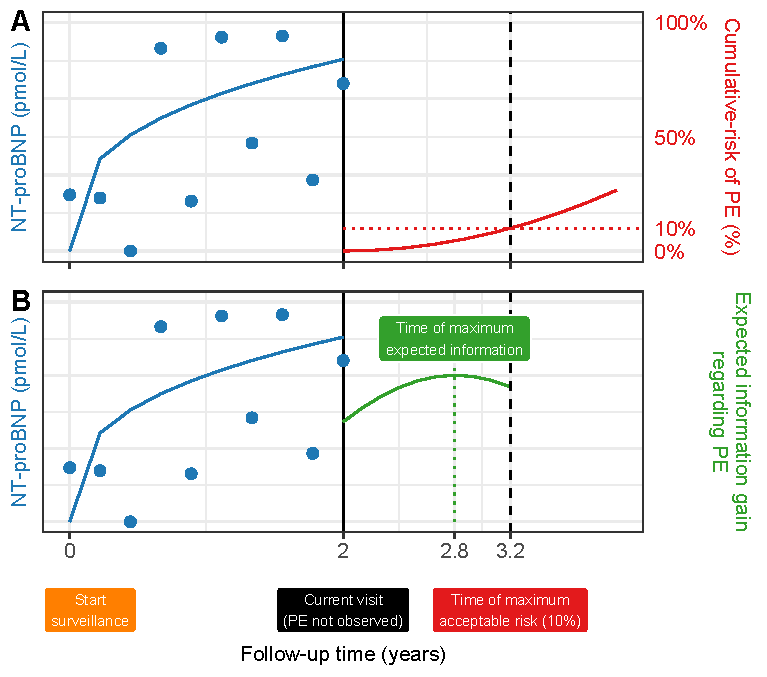
\includegraphics{contents/c6/images/c6_fig1.pdf}
\caption{\textbf{Illustration of personalized scheduling of biomarker measurements.} We plan NT-proBNP measurements until the cumulative-risk of PE (primary endpoint) at three months from the current visit is more than 10\%. \textbf{Panel~A}: Example patient with longitudinal NT-proBNP measurements and fitted profile (in blue). The time of the current visit, on which PE was not observed, is year 2. Using NT-proBNP and time of current visit data, we derive a personalized cumulative-risk profile for the patient (in red). This risk profile reaches the 10\% level at year 3.2, and hence, we are allowed to schedule new measurements until year 3.2. \textbf{Panel~B}: We calculate the expected information gain in the patient's prognosis if a new NT-proBNP measurement is done at a future time point between the current visit at year 2 and the time of the maximum acceptable risk of 10\% at year 3.2. The time of maximum expected information gain, is year 2.8, and hence, we schedule new NT-proBNP measurement at year 2.8.}
\label{c6:fig:1}
\end{figure}

\subsection{Simulation study}
After constructing the joint model and defining the thresholds needed for scheduling personalized screening visits, we proceeded to compare the personalized screening schedule to a fixed screening schedule. For the fixed schedule, we chose trimonthly intervals, in accordance with the design of the Bio-SHiFT study and daily clinical practice. Since our existing data were collected using this fixed screening schedule and hence no ‘real' data on personalized screening intervals was available, the advantages of a personalized screening design were assessed by means of a simulation study. 
We first simulated a dataset containing 750 patients. These 750 simulated patients had baseline characteristics and NT-proBNP profiles similar to the 263 patients included in the Bio-SHiFT since we simulated using the joint model fitted to the Bio-SHiFT data. We divided this data into training (700 patients), and testing (50 patients) set. For the training patients, using the joint model fitted to the Bio-SHiFT data, we generated NT-proBNP measurements at fixed follow-up time points. This schedule is similar to the schedule of the Bio-SHiFT study. We also generated a true PE time for these patients, as well as a random non-informative censoring time. Subsequently, we fitted a new joint model for these patients and, then, used this model to develop NT-proBNP measurement schedules for the test patients. To this end, in the test patients, we only generated the true PE time. Using such a design ensured that the ‘new' patients (n=50) are comparable to the ‘existing' patients (n=700) on which the model is based; if we had used the ‘real' patients (n=263 from the Bio-SHiFT study), this might not have been the case. 

Thus, for each of the 50 patients in the test set, we aimed to compare the efficacy of scheduling NT-proBNP measurements according to a fixed screening design and a personalized screening design. For the personalized screening design, the first three simulated NT-proBNP measurements were considered a given, in order to have a ‘run-in period' for the patients' longitudinal profile of NT-proBNP, since if we have a longitudinal profile available we can apply the aforementioned stepwise approach of personalized scheduling. Apart from using the risk-threshold of 7.5\% over a 3-month period, we repeated the analysis using 5\% and 10\% risk thresholds. We did so because 5\% is a lower cumulative-risk, and consequently, scheduling will stop earlier than in case of a 7.5\% risk threshold, which will give us more time to intervene with respect to the true PE time. Conversely, 10\% is a higher risk percentage than 7.5\%, and hence schedules based on the former will give us less time. 

The performance of the personalized and fixed screening schedules was compared using two outcome measures, namely, the start of the high-risk interval and the number of scheduled measurements. The high-risk interval was defined as the estimated intervention time minus the true event time (in months) (Fig. 1D). Thus, the schedule that showed a high-risk interval that was larger in absolute terms (i.e., more negative) was preferred, because such a high-risk interval enables timely intervention. In addition, assuming that the costs of NT-proBNP measurements and outpatient visits remained the same during follow-up, we prefer a procedure that requires the fewest possible repeated measurements (Supplemental Materials). All analyses were performed with R statistical software using package JMBayes~\citep{rizopoulosJMbayes}.
\section{Results}
\label{c6:sec:results}

\subsection{Baseline characteristics}
The mean age of the patients was 66.7 years, and 71.9\% were men (Table~\ref{c6:table:1}). Most patients were in NYHA class I or II (73.8\%). The median baseline NT-proBNP value was 137.3 pmol/L (IQR: 51.7-272.6). A total of 2022 NT-proBNP measurements were performed during follow-up before the PE occurred. The PE occurred in 70 patients (26.6\%). The median maximum follow-up time was 2.1~(IQR: 1.2--2.4) years.

\begin{table}
\small
\centering
\caption{\textbf{Summary of the Bio-SHiFT dataset}. The primary study endpoint (PE) was defined as the composite of cardiac death, cardiac transplantation, left ventricular assist device implantation, or hospitalization for heart failure, whichever occurred first. Abbreviations: NYHA is New York Heart Association Classification~\citep{bredy2018new}; IQR is interquartile range.}
\label{c6:table:1}
\begin{tabular}{p{8cm}r}
\toprule
\textbf{Characteristic} & Value\\
\midrule
Total patients & 263\\
\emph{PE (primary endpoint)} & 70\\
\midrule
Total NT-proBNP measurements & 2022\\
Median NT-proBNP (pg/mL) & 110.3 (IQR: 38.5--240.9)\\
Median age at inclusion (years) & 67.9 (IQR: 58.9--75.8)\\
Median BMI at inclusion & 26.5 (IQR: 24.4--30.1)\\
Median NYHA (assumed continuous) & 2 (IQR: 1--3)\\
$\mbox{Gender} = \mbox{Female}$ (\%) & 74/263 (28.1\%)\\
$\mbox{Renal failure history} = \mbox{Yes}$ (\%) & 136/263 (51.7\%)\\
$\mbox{Type-II diabetes mellitus} = \mbox{Yes}$ (\%) & 81/263 (30.8\%)\\
\midrule
Median maximum follow-up per patient (years) & 2.1 (IQR: 1.2--2.4)\\
Median \#NT-proBNP per patient & 9 (IQR: 5--10)\\
\bottomrule
\end{tabular}
\end{table}

\subsection{Association between temporal patterns of NT-proBNP and the PE}
Serially measured NT-proBNP was associated with the PE (univariable HR per doubling of NT-proBNP:~2.13, 95\%CI:~1.81--2.53, p<0.001). After adjustment for age, gender, diabetes mellitus, NYHA class, body mass index, and renal function, serially measured NT-proBNP remained independently associated with the PE (adjusted HR per doubling of NT-proBNP:~2.20, 95\%CI~:1.84--2.68, p<0.001). Two examples of dynamic risk assessment of individual patients from the Bio-SHiFT dataset based on the joint model are demonstrated in Supplemental Materials, Figure 1A-B. 

\subsection{Fixed versus personalized screening schedule: high-risk interval and number of measurements}
The median follow-up time of the 750 patients in the simulated dataset was 1.76 years~(IQR:~1.42--2.24); mean~(standard deviation) was 1.85~(0.63) years and the maximum was~3.5 years. The personalized schedule used fewer measurements as compared to the fixed (Panel~A, Figure~\ref{c6:fig:2}). The personalized schedule used a median of 7~(IQR:~7--8) and the fixed schedule, a median of~9~(IQR:~8--10) measurements. Corresponding cost estimates are demonstrated in the Supplemental Materials. The start of the high-risk intervals for the fixed and personalized screening schedules are depicted in Figure 2B. The personalized and fixed schedules showed similar results, i.e., the difference between the estimated intervention time compared to the `true' event time was a median of~6.6~(IQR:~4.5--11.3) months for the personalized and a median of~6.3~(IQR:~4.2--10.3) months for the fixed schedule (Panel~B, Figure~\ref{c6:fig:2}). In both schedules, scheduling of new sampling moments was stopped in order to undertake appropriate action, well in time before the event occurred.

\begin{figure}
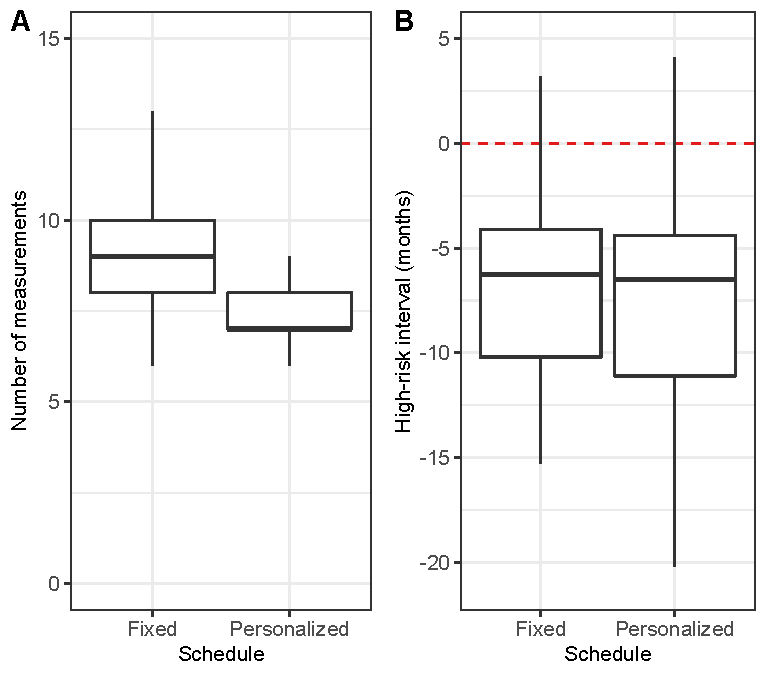
\includegraphics{contents/c6/images/c6_fig2.pdf}
\caption{\textbf{Total NT-proBNP measurements and high-risk interval (months) preceding the primary endpoint (PE)} for fixed (quarterly measurements) and personalized schedules. Results are based on a realistic simulation study of 263 test patients. NT-proBNP is measured as per personalized and fixed schedules, until a patient's cumulative-risk of obtaining PE in the subsequent three months is above 7.5\%. The boxplot for the number of measurements in Panel~A is made using data of all simulated patients. The boxplot for the high-risk interval (the difference between the time at which NT-proBNP measurements are stopped and the true simulated PE time) in Panel~B, is based on only those patients who observe PE. In Panel~B a zero high-risk interval (dashed red line) indicates that no time is available for intervention before occurrence of PE.}
\label{c6:fig:2}
\end{figure}

Results of the analyses using risk thresholds of consecutively 5\% and 10\% over three months are depicted in the Supplemental Materials, Figure~\ref{c6:fig:app1}, and Figure~\ref{c6:fig:app2}, respectively. Based on a risk threshold of 5\% over three months, the fixed and personalized screening schedules demonstrated similar results for the high-risk interval. However, again, the personalized screening schedule used fewer measurements as compared to the fixed screening schedule. The same was true for the risk threshold of 10\%. In case of a risk threshold of 5\% over three months, we found that the start of the high-risk interval was further away from the true event time as compared to a risk threshold of 7.5\% over three months. Conversely, in case of a risk threshold of 10\% over three months, the start of the high-risk interval was closer to the true event time as compared to a risk threshold of 7.5\% over three months. These results comply with the increase in the risk threshold.
\section{Discussion}
\label{c6:sec:discussion}
This study aimed to optimally schedule NT-proBNP measurements for individual patients with CHF while maximizing the gain in prognostic information and reducing costs. Furthermore, to compare the efficacy of such personalized scheduling with fixed scheduling. We found that over a median follow-up time of 1.8 years, personalized scheduling required fewer NT-proBNP measurements per patient as compared to fixed scheduling while demonstrating similar performance regarding the prevention of adverse cardiac events. Since personalized scheduling required fewer measurements, this approach is expected to reduce related health care costs as well as patient burden compared to fixed scheduling.

The findings from our study carry important implications for future trials on biomarker-guided therapy. Previous biomarker-guided trials have generally used predefined sampling intervals and target levels~\citep{khan2018does,felker2017effect}. We show that, by using a personalized approach for scheduling NT-proBNP, timely intervention is enabled while using fewer NT-proBNP measurements as compared to a fixed schedule. Even though our fixed schedule consisted of rather frequent (trimonthly) NT-pro-BNP measurements, the high-risk interval identified by the personalized schedule was similar. On top of this, the fixed schedule was outperformed by the personalized schedule in terms of the number of measurements needed per patient to obtain this result. Maximizing information gain by estimating prognosis in an individual and optimal manner, while minimizing healthcare burden, may provide novel opportunities for timely adaptation of treatment. Future trials on natriuretic peptide-guided therapy for chronic heart failure may benefit from incorporating personalized screening intervals and personalized biomarker value targets; tailoring therapeutic interventions using this approach may reveal benefits that could not be demonstrated by previous trials, by nature of their design. 

Previous studies on personalized scheduling of blood sampling moments for measurements of biomarkers of disease are scarce, but this topic seems to be gaining attention recently. Personalized scheduling has been applied to patients undergoing aortic allograft root implantation~\citep{rizopoulos2016personalized}. Similarly to our study, this study used joint modeling. Aortic gradient levels were measured according to a fixed screening schedule. The authors demonstrated that personalized scheduling of aortic gradient assessments required fewer measurements and also performed better regarding the prevention of recurrent events as compared to fixed scheduling. Recently, personalized schedules for reducing the number of biopsies in low-risk prostate cancer patients have also been developed~\citep{tomer2019personalized}. Altogether, these promising results in other disease areas concur with our conclusion that personalized screening intervals carry the potential to improve patient monitoring and to ultimately individualize and herewith improve treatment.

\subsection{Limitations}
Several aspects of this study warrant consideration. First, we made several assumptions when developing the model, defining the thresholds, and setting up of the simulation study. However, in a sensitivity analysis, we performed the simulation study for three different risk thresholds, and the results remained essentially unchanged. Second, in our investigation, we performed a so-called demonstration, meaning that the analysis was performed on one `test' set of 50 patients, and was not repeated. We performed a demonstration because we aimed to provide a proof-of-concept here. A study with multiple test sets should be performed to validate our findings further. Although, it should be noted that such repeated estimations pose a heavy computational burden. Third, we did not account for the costs of implementation. Finally, while the concept of personalized screening intervals we present here seems promising, whether it would actually lead to the prevention of adverse events remains to be investigated in a clinical trial.

\subsection{Conclusions}
In conclusion, this study demonstrates for the first time that personalized scheduling of NT-proBNP measurements in patients with CHF, as compared to fixed scheduling, shows similar performance with regard to prevention of recurrent events but requires fewer NT-proBNP measurements. If such personalized scheduling were to be applied in natriuretic peptide-guided therapy, these benefits might translate into improved outcomes. Therefore, a clinical trial incorporating personalized scheduling should be considered.
\section*{Author Contributions}
\noindent \emph{Study Design}: Akkerhuis, Umans, Boersma, Kardys\\
\noindent \emph{Data analysis}: Schuurman, Tomer\\
\noindent \emph{Drafting Manuscript}: Schuurman, Tomer\\
\noindent \emph{Analytics Strategy}: Rizopoulos, Kardys\\
\noindent \emph{Directing Implementation}: Umans, Kardys\\
\noindent \emph{Quality Control}: Kardys\\
\noindent \emph{Data Interpretation}: All authors\\
\noindent \emph{Critical revision of manuscript for important intellectual content}: All authors

\section*{Appendix}

\begin{subappendices}
\section{Details: Materials and Methods}
\subsection{Study procedures and outcome measures}
During their baseline and follow-up visits, all patients were evaluated by research physicians, who collected information on CHF-related symptoms, New York Heart Association (NYHA) class, and performed a physical examination. Information on CHF etiology, left ventricular ejection fraction, cardiovascular risk factors, medical history, and treatment was retrieved primarily from hospital records and was checked in case of ambiguities. History of cardiovascular and other comorbidities was defined as clinical diagnosis thereof reported in the hospital records.

\subsection{Blood sampling and NT-proBNP measurement}
Blood samples were processed and stored at a temperature of -80 degrees C within 2 hours after blood collection. When applicable, samples were transported to the central laboratory (Erasmus MC, Rotterdam, the Netherlands) under controlled conditions (at a temperature of -80 degrees C) until batch analysis was performed. Accordingly, results of the biomarker assays were not available to treating physicians at the time of the outpatient visits and hence did not alter patient care. Plasma NT-proBNP was analyzed using an Electrochemiluminescence immunoassay (Elecsys 2010; Roche Diagnostics, Indianapolis, IN), which measures concentrations ranging from 5 to 35000 ng/L. 

\subsection{Joint Modeling}
We utilized a joint model to estimate the association between longitudinally measured NT-proBNP and clinical outcomes. A joint model combines a linear mixed-effect (LME) model for longitudinally measured data with a Cox regression model for time-to-event data. The use of joint modeling was motivated by the following considerations. In the Bio-SHiFT study, NT-proBNP levels were measured trimonthly until the PE occurred, or until the patient was censored. Thus, naturally, patients who experienced a PE had NT-proBNP measurements available over a shorter time-course than those who did not experience a PE; or in other words, further NT-proBNP measurements could be considered as missing due to occurrence of the PE. However, commonly used methods to model such longitudinal data, for example, linear mixed-effect (LME) models, assume that missing data is non-informative with regard to a patient's health status. In other words, they do not account for the fact that patients with missing NT-proBNP values are more likely to have higher NT-proBNP levels (if hypothetically, we would have been able to observe them). This may lead to bias in the parameter estimates. In addition, a classical time-dependent Cox regression may be used in order to measure the impact of NT-proBNP on the PE. However, due to the aforementioned issue, the time-dependent Cox model may also be biased. To correctly estimate the effects, the parameters of these two types of models are required to be estimated jointly. We did so by applying the joint model.

\subsection{Costs}
Based on the number of scheduled measurements by the personalized and the fixed scheduling approach, we compared the cost estimates from the perspective of Erasmus MC as well as the perspective of society at large for both scheduling approaches. Cost estimates from the perspective of the Erasmus MC included costs of NT-proBNP sampling and measurement, as well as visiting the Cardiology outpatient clinic, at this particular institution~\citep{kanters2017update,hakkaart2015costing}. Cost estimates from the perspective of society at large included average Dutch cost estimates of NT-proBNP sampling and measurement and average Dutch cost estimates of visiting a Cardiology outpatient clinic. Moreover, patients' travel costs and patients' production losses associated with visiting the outpatient clinic were included~\citep{kanters2017update,hakkaart2015costing}.

\section{Supplemental Results}
\subsection{Fixed versus personalized screening schedule: costs}
Costs are depicted in Table~\ref{c6:table:app1}. From the perspective of the Erasmus MC, the costs associated with a visit to the Cardiology outpatient clinic, including blood sampling and NT-proBNP measurement, were €182.1 Thus, since the personalized screening schedule required two visits less than the fixed schedule (Figure~\ref{c6:fig:1}), from the perspective of the Erasmus MC the costs saved by personalized scheduling were on average €364 per patient, over a mean follow-up of 1.76 years (€207 saved per patient per year).

From the perspective of society at large, costs for visiting the outpatient clinic, blood sampling, and NT-proBNP measurement were €106.1 Travel costs and production losses amounted to €6 and €33, respectively. Altogether, costs per visit amounted to €145, with, on average, €290 saved per patient by personalized scheduling versus fixed scheduling, again over a mean follow-up of 1.76 years (€165 saved per patient per year).

In The Netherlands, the prevalence of CHF is estimated at 227,000 patients (\url{www.nivel.nl/node/4309}). In this context, personalized screening could reduce the involved annual costs by approximately €37 million from the perspective of society at large.

\begin{table}
\small
\centering
\caption{\textbf{Cost estimates from the perspective of the Erasmus MC and society at large.} Abbreviations are, CHF: chronic heart failure; NL: The Netherlands; NT-proBNP: N-terminal pro-B-type natriuretic peptide.}
\label{c6:table:app1}
\begin{tabular}{p{6cm}rr}
\toprule
\textbf{Costs} & Erasmus MC (€) & Society at large (€)\\
\midrule
NT-proBNP measurement, per measurement & 19 & 15\\
Visit to outpatient clinic, per visit & 163 & 91\\
Travel costs, per visit	& - & 6\\
Production loss costs, per visit & - & 33\\
Total costs, per visit & 182 & 145\\
\midrule	
Total costs for fixed schedule (median of 9 measurements) & 1638 & 1305\\
Total costs for personalized schedule (median of 7 measurements) & 1274 & 1015\\
Costs saved by personalized scheduling, per patient & 364 & 290\\
Annual costs saved by personalized scheduling (prevalence CHF in NL estimated at 227,000 patients) & - & 37,455,000\\
\bottomrule
\end{tabular}
\end{table}

\begin{figure}
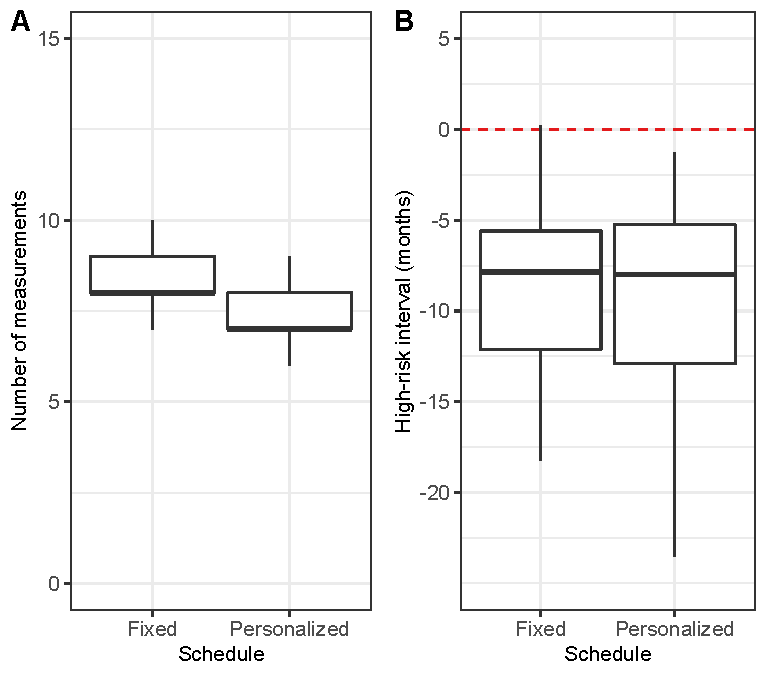
\includegraphics{contents/c6/images/c6_fig_app1.pdf}
\caption{\textbf{Total NT-proBNP measurements and high-risk interval (months) preceding the primary endpoint (PE)} for fixed (quarterly measurements) and personalized schedules. Results are based on a realistic simulation study of 263 test patients. NT-proBNP is measured as per personalized and fixed schedules, until a patient's cumulative-risk of obtaining PE in the subsequent three months is above 5\%. The boxplot for the number of measurements in Panel~A is made using data of all simulated patients. The boxplot for the high-risk interval (the difference between the time at which NT-proBNP measurements are stopped and the true simulated PE time) in Panel~B, is based on only those patients who observe PE. In Panel~B a zero high-risk interval (dashed red line) indicates that no time is available for intervention before occurrence of PE.}
\label{c6:fig:app1}
\end{figure}

\begin{figure}
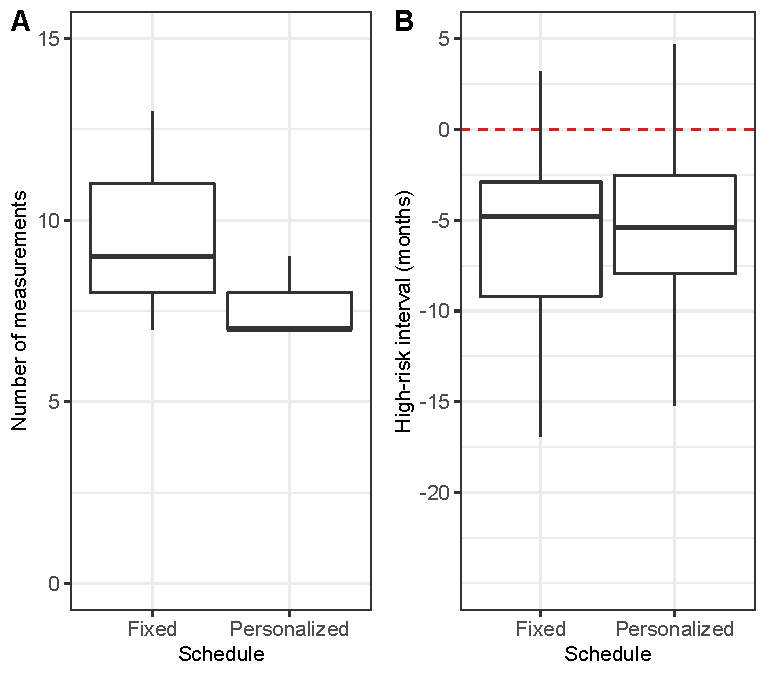
\includegraphics{contents/c6/images/c6_fig_app2.pdf}
\caption{\textbf{Total NT-proBNP measurements and high-risk interval (months) preceding the primary endpoint (PE)} for fixed (quarterly measurements) and personalized schedules. Results are based on a realistic simulation study of 263 test patients. NT-proBNP is measured as per personalized and fixed schedules, until a patient's cumulative-risk of obtaining PE in the subsequent three months is above 10\%. The boxplot for the number of measurements in Panel~A is made using data of all simulated patients. The boxplot for the high-risk interval (the difference between the time at which NT-proBNP measurements are stopped and the true simulated PE time) in Panel~B, is based on only those patients who observe PE. In Panel~B a zero high-risk interval (dashed red line) indicates that no time is available for intervention before occurrence of PE.}
\label{c6:fig:app2}
\end{figure}
\end{subappendices}

\clearpage
\bibliographystyle{apalike}
\bibliography{c6_bib}
\part{Summary}
\chapter[General Discussion][General Discussion]{General Discussion}
\label{c7}

\cleardoublepage

\section{Background}
\label{c7:sec:background}
Low-risk chronic non-communicable disease (e.g., localized prostate cancer, low-risk dysplasia) patients often undergo repeated invasive \emph{tests} (biopsies, endoscopies, etc.) for confirming disease \emph{progression}. A progression is a non-terminal event upon which patients usually undergo serious treatments, e.g., surgery, radiotherapy. Typically, invasive tests are conducted routinely according to a one-size-fits-all (e.g., yearly) fixed schedule~\citep{bokhorst2015compliance,choi2012screening,krist2007timing,mcwilliams2008surveillance,henderson2011surveillance}. Invasive tests are burdensome~\citep{loeb2013systematic,krist2007timing} but also indispensable for timely detection of disease progression. Specifically, frequent one-size-fits-all test schedules promise shorter time delays in observing progression at the cost of imposing an extra burden on patients who progress slowly. The vice versa holds for infrequent tests. Our aim in this thesis was to balance better the number of tests (burden) and time delay in detecting progression (shorter is beneficial) than fixed schedules. To this end, we developed and applied statistical methods for scheduling invasive diagnostic tests (e.g., biopsies, endoscopies) in a personalized manner.

To create personalized test schedules we first utilized a statistical model to predict a patient's cumulative-risk of progression over the whole follow-up period based on his accumulated clinical data. This risk profile manifested the transition of a patient's disease state over time from low-risk to progressed. Hence, subsequently, we used it to guide the timing of future invasive tests. Specifically, we derived personalized test schedules by optimizing utility functions of clinical parameters of interest (Chapters~\ref{c2}, \ref{c3}, and \ref{c4}) under the estimated patient-specific cumulative-risk of progression. We also employed the cumulative-risk of progression to assess the widely utilized approach of scheduling invasive tests using partially observable Markov decision processes (Chapter~\ref{c4:appendix:pomdp}). We then implemented personalized biopsy schedules for real patients of the seven largest prostate cancer active surveillance programs (Chapter~\ref{c5}) in a web-application (\url{https://emcbiostatistics.shinyapps.io/prias_biopsy_recommender/}). The use of personalized schedules is not limited to invasive tests only. In this regard, we also applied them for planning the NT-proBNP biomarker (a simple blood test) measurements in chronic heart failure patients (Chapter~\ref{c6}).
\section{Subgoals and Research Questions}
\label{c7:sec:subgoals}
\subsection{Statistical Modeling Framework to Process Observed Patient Data}
We used the framework of joint models for time-to-event and longitudinal data~\citep{rizopoulos2012joint,tsiatis2004joint} to process a patient's data and predict his patient's cumulative-risk of progression. We chose this for three main reasons. First, joint models utilize patient-specific random-effects and are hence inherently personalized. Second, they accommodate outcomes of various types, including longitudinally measured, baseline patient data, and results from previous invasive tests. Third, they update risk predictions automatically over follow-up as more patient data become available. 

There are some limitations of the joint models that we utilized. First, in our model, we selected predictors based on existing hypotheses regarding the clinical relevance of the predictors. However, such hypotheses can change with time, e.g., PSA velocity~\citep{vickers2014commentary}. An alternative is choosing model predictors based on their predictive ability. Second, we ignored competing-risk scenarios and estimated only cause-specific cumulative-risk of progression. Third, our model did not account for the sampling error and inter-observer variation in invasive test results. However, these limitations apply only to the model, i.e., the scheduling methodology remains the same, even if a better model is employed.

\subsection{Pros of Cons of Different Utility Functions}
\paragraph{Utility functions: squared and absolute loss, Parameter of interest: time of progression} In Chapter~\ref{c2}, we optimized two commonly used loss functions, namely, expected squared and absolute loss~\citep{robertBayesianChoice} for the time of progression to decide the time of the next invasive test. These loss functions plan an invasive test at the estimated mean (square loss) and median (absolute loss) time of progression of a patient. There are two limitations to this method. First, due to the limited follow-up period of real-world studies, only a restricted version of the mean time of progression can be calculated, which has no straightforward interpretation. Second, depending upon the standard deviation of the posterior predictive distribution of time of progression, the difference between the actual and mean time of progression can be substantial. Both mean and median time of progression may sound suitable when interpreted as the central tendency of the distribution for time of progression. However, they also represent the time at which a patient has a 50\% risk of progression, which may seem large clinically.

\paragraph{Utility function: multi-linear loss (risk-based tests), Parameter of interest: time of progression} Squared and absolute loss penalize equally a planned invasive test that exceeds or falls short of the time of progression. However, patients may weigh these two scenarios unequally, especially because multiple tests before the actual time of progression can be burdensome. In this regard, a multi-linear loss function (Chapter~\ref{c2}) can be used. This loss function plans a test at a time point at which the patient's risk of progression is equal to a particular risk threshold. Smaller risk thresholds plan a test earlier than higher risk thresholds. In other words, smaller risk thresholds penalize exceeding the time progression more than falling short of the time of progression. 

The main caveat in such risk-based test decisions (Chapter~\ref{c3}) is the choice of risk threshold. This threshold may be chosen by patients and/or doctors according to how they weigh the relative harms of doing an unnecessary test versus a missed disease progression (e.g., 10\% threshold means a 1:9 ratio) if the test is not conducted~\citep{vickers2006decision}. Threshold choice can also be partly data-driven, e.g., based on the threshold's estimated sensitivity and specificity of diagnosing progression. In this regard, it is also possible to choose risk thresholds using more sophisticated measures than just sensitivity or specificity, e.g., Youden's index, F1 score~\citep{lopez2014optimalcutpoints}. However, a critical limitation of such measures is that they may automatically select a risk threshold with clinically unsuitable sensitivity and specificity. Also, typically such measures are difficult to interpret.

\paragraph{Utility function: Partially observable Markov decision process (POMDP) value function} In Chapter~\ref{c4:appendix:pomdp} we explored the framework of POMDP to schedule invasive tests. The choice of POMDP was motivated by its wide usage in numerous optimal screening and surveillance test schedules for chronic diseases~\citep{steimle2017markov,denton2018optimization}, and especially for nearly all types of cancers~\citep{alagoz2010operations}. 

In general, POMDPs utilize estimates from previously conducted studies or surveys to build a disease state transition model. In this work, we did not have to rely on existing studies as we made a joint model for modeling the patient's disease state and the associated clinical data. We integrated joint models with POMDPs by replacing the Bayes-rule based belief (risk of disease progression, see Equation~\ref{c4:eq:belief_jm}) update of POMDPs, with the dynamic predictions~\citep{rizopoulos2017dynamic} of cumulative-risk of progression from joint models. This had the advantage that it also personalized the POMDP. Concerning the use of clinical data, POMDPs assume that the probability distribution of future longitudinal data adds extra information over observed data. However, we estimated the posterior probability distribution of future longitudinal data based on observed data using the joint model. Hence, sampling a new observation from the future distribution and using it to update belief adds no information. This was not our sole reason for ignoring the posterior probability distribution of future longitudinal data. Another was that POMDP algorithms suffer from the curse of dimensionality with continuous longitudinal outcomes~\citep{sunberg2018online}.

We also observed a more substantial drawback of POMDPs lying in their very flexible specification. Specifically, in a simple POMDP with binary test/no test decisions, and binary disease state (low-risk, progressed), it can be shown that there exist infinite possible rewards result in the same optimal schedule (Chapter~\ref{c4:appendix:pomdp}). Typically POMDP rewards are chosen based on survey results~\citep{denton2018optimization} and translated as quality-adjusted life-years saved. However, with infinite optimal reward sets, any reward set can be cherry-picked, including those that correspond to (improbable) thousands of quality-adjusted life-years saved. Hence, POMDPs may find the most optimal schedule, but to achieve that, the choice of suitable rewards is tough in practice.

\paragraph{Utility function: Euclidean distance, Parameters of interest: expected number of tests and time delay in detecting progression} Motivated by the POMDP framework we improved over planning one future test at a time (Chapter~\ref{c2}~and~\ref{c3}), by replacing it with a whole schedule of tests planned until a maximum future time point (e.g., end of the study period) in Chapter~\ref{c4}. To this end, we made risk threshold based test decisions iteratively at each future follow-up visit (e.g., future visits for biomarker measurement) of the patient. An important question, in this case, is which risk threshold yields the optimal schedule? To assist patients and doctors in this endeavor, we proposed a utility function to find the optimal risk threshold based schedule. The utility function was the Euclidean distance between a risk-based schedule and a perfect schedule (one test planned at the exact time of progression) in a bi-dimensional space of the expected number of tests and time delay in detecting progression. While we included only risk-based schedules in the Euclidean space, given $L$ future visits of a patient, the Euclidean distance can be used to find the optimal schedule among all $2^L$ possible schedules.

The main advantage of this approach is that we directly minimize quantities that manifest burden and benefit. Second, personalized schedules get updated with newly collected data over follow-up. Third, Euclidean distance is easier to understand compared to squared loss or the recursive POMDP value function. A drawback of our approach is that we are only able to schedule tests up to a maximum horizon time. Another caveat is that a fair comparison of time delays between different schedules for the same patient requires a compulsory test at a common horizon time point in all schedules.

\subsection{Criteria for Comparison of Schedules}
An important question for patients and doctors is if personalized schedules are any better than fixed schedules. Especially if personalized schedules improve upon patient deaths and/or progression to an advanced disease state (e.g., metastasis) compared to fixed schedules. However, to our knowledge, currently, there are no running studies that compare personalized versus fixed schedules. Also, reliable data on the number of patient deaths are difficult to obtain in low-grade diseases. This is because, in such diseases, the prevalence of death from disease can be quite low. For example, in the PRIAS prostate cancer dataset, only two out of 7813 patients were reported to die from prostate cancer.

In search of the criteria for comparison of schedules, in Chapter~\ref{c4:subsec:kappa_selection} we proposed a method to calculate expected number of tests (burden) per schedule and expected time delay in detecting progression (shorter is beneficial) for any schedule, fixed or personalized. These two are easily-quantifiable surrogates for important clinical aspects, such as the window of opportunity for curative treatment, risk of adverse downstream outcomes, quality-adjusted remaining lifetime, and additional complications in treating a delayed progression. Based on these two quantities, patients/doctors can compare any schedule with any other and decide which schedule suits them best. Both expected number of tests and expected time delay in detecting progression are calculated in a personalized manner. That is, two patients may be prescribed the exact same schedule of tests, but their expected time delay in detecting progression and the expected number of tests will depend on their disease progression risk profile.

\subsection{Factors Affecting Performance of Personalized Schedules}
We utilized the estimated cumulative-risk of disease progression for developing personalized schedules throughout this work. Thus, how accurately this risk profile resembles the actual disease state dictates the performance of the personalized schedules. In this regard, both the quality of the clinical data and the accuracy of the model are important. For example, in the prostate cancer surveillance scenario, we found that prostate-specific antigen (PSA) and its derivatives, such as PSA velocity, were not very strong predictors of progression (Chapter~\ref{c5}). Besides, the PSA measurement error was best modeled with a t-distribution with three degrees of freedom. As a result, until a rise in PSA was evident via multiple observations and the surge was sharp as well, the predicted risk profile remained almost the same. Another effect of this was that once a negative result was obtained on a biopsy, a patient's predicted risk remained low until PSA consistently showed a sharp rise. Consequently, our model discriminated poorly (Chapter~\ref{c5:appendix:validation_res}) between patients who obtained progression versus patients who did not obtain progression within a short time period of their last biopsy (e.g., an year). Overall, while building a model for personalized schedules, the focus should be on predictive ability of the model.

\subsection{Reusing a Test Scheduling Framework Across Different Cohorts and Diseases}
The utility functions and methodology we developed in this work is generic for scheduling tests in both screening and surveillance scenarios. It is also not necessary to rely only on joint models. The proposed utility functions only require an estimate of cumulative-risk of progression. While we focused on balancing the number of tests and time delay in detecting progression, users can extend the proposed methodology to include other aspects such as quality-adjusted life years. Our methodology may work differently in certain diseases. For example, in Barrett's esophagus~\citep{choi2012screening}, longitudinal data (e.g., p53 and SOX2 protein expressions) is collected when endoscopy (invasive test) is conducted. Consequently, risk predictions and personalized schedules do not update unless a test is conducted. Based on our findings from validation of the PRIAS (prostate cancer data introduced in Chapter~\ref{c1:subsec:PRIAS}) based model in external datasets (Chapter~\ref{c5:appendix:validation_res}), a model may require recalibration (e.g., of baseline-risk) before reusing in other cohorts. Alternatively, one may fit a new model to the new cohort before using the model for personalized schedules.
\section{Recommendations for Practice, and Future Improvements}
\label{c7:sec:future_research}
Based on the work done in this thesis, we have certain recommendation for practitioners as well a list of improvements that may be researched in future. We next provide these recommendations and improvements in each of the four steps of creating invasive test schedules (defined in Chapter~\ref{c1:subsec:goal}). These are, namely, processing the observed data of the patient, choosing the reward/utility/loss function and the corresponding clinical parameters, comparing proposed personalized schedules with currently practiced schedules, and implementing personalized schedules in a computer application for practitioners.

\subsection{Observed Data of the Patient}
Our overall recommendation while developing a model for personalized schedules is to focus on the predictive performance of the model. For example, in the prostate cancer surveillance joint model, we used a limited set of predictors (e.g., PSA value and velocity). However, this did not necessarily lead to the model with the best prediction error, and/or capacity of discrimination (e.g., the area under the receiver operating characteristic curve) between patients who are progressing and non-progressing patients. In this regard, although a joint model is a suitable candidate for modeling both longitudinal and time-to-event data, practitioners may also explore other models, and strive to achieve the best predictions. In addition, there are four broad areas of improvement in modeling observed data of the patient than the standard joint model we used.

\paragraph{Sampling error} In general invasive procedures such as biopsies are prone to sampling error, especially when the site for sampling the tissues is not chosen carefully. In this regard,~\citet{coley2017} have proposed a joint model that predicts the time of actual disease progression given the time of observed progression. Actual progression means progression in the absence of sampling error, e.g., progression based on complete tumor such as via surgical removal, rather than biopsy samples.

\paragraph{Inter-observer variation} Invasive test results are also prone to inter-observer variation. Models that have been proposed~\citep{balasubramanian2003estimation} to handle this problem require an estimate of the size and direction of the inter-observation variation. However, if the inter-observer variation for a test is inherently large, then overall model parameter estimates for risk of progression may also inflate.

\paragraph{Recurrent cancer} We did not consider the scenario of surveillance of recurrent occurrence of progression (e.g., recurrent breast cancer). Although, if a model predicts risk of progression while accounting for recurrent events~\citep{rizopoulos2012joint}, the scheduling methodology that we proposed may not change.

\paragraph{Competing-risks} In this work, we assumed all competing events to be non-informative censoring. However, treatment without progression or death may occur in a substantial number of patients. This affects our methodology in three ways. First, while creating risk-based schedules; second, during the calculation of the expected number of tests given a schedule; and third, in the calculation of expected time delay in detecting progression given a schedule. Among these, schedules based on cause-specific cumulative-risk may be alternatively obtained using the cumulative-incidence function~\citep{andrinopoulou2017combined, putter2007tutorial}. The expected number of tests requires a model in which all events are combined to form a composite event. This is because the occurrence of any of the competing events will stop surveillance. On the other hand, time delay in detecting progression may only be defined if progression occurs before any other competing event.

\subsection{Choice of Reward/Utility Function}
The majority of the scheduling methods we explored in this work optimized the expected value of a utility function. Although, another key aspect is the variance of the utility. This is because a schedule with sub-optimal expected utility but lower utility variance may seem more trustworthy owing to its consistency. For example, the squared loss has a high variance in delay in detecting progression despite having expected delay equal to zero (Chapter~\ref{c2}). Second, we relied on the number of invasive tests and time delay in detecting disease progression as measures of burden and benefit of scheduling an invasive test. However, it is also important to consider patient anxiety, risk of complications, risk of non-compliance, and quality-adjusted life-years (QALY). Among these, the reference measure in a cost-utility analysis is QALY~\citep{sassi2006calculating}. Although it can be included in the utility functions we proposed (Chapter~\ref{c4}), the biggest challenge is calculating QALYs correctly in different disease surveillance.

\paragraph{Optimizing the schedule of invasive tests and longitudinal outcomes together} In Chapters~\ref{c2} to~\ref{c5}, we optimized the schedule of invasive tests, whereas in Chapter~\ref{c6} we optimized the schedule of the longitudinal outcome. In diseases such as chronic heart failure (Chapter~\ref{c6}), being able to measure the longitudinal outcome also indicates the survival of the patient. This is because if the patient obtains the event (cardiac failure), the longitudinal outcome cannot be measured. Whereas in a disease such as Barrett's esophagus, longitudinal outcomes are also measured via endoscopy (invasive). Hence, there is no need to optimize the schedule of invasive tests and the longitudinal outcomes separately. Conversely, in prostate cancer active surveillance, longitudinal outcomes can be measured even after patient obtains progression because progression in prostate cancer active surveillance is a non-terminal event. Hence, an interesting question is if we can optimize both the schedule of invasive tests and multiple longitudinal measurements together. 

Optimizing the schedule of invasive tests and longitudinal outcomes together has the potential to reduce patient burden even further. However, it has certain caveats too. For example, in Chapter~\ref{c5}, we observed that PSA is not a strong indicator of progression. Thus, fewer PSA measurements will mean increased variance of estimates of cumulative-risk of progression. On the other hand, in diseases where the biomarker is a strong indicator of progression, measuring it less frequently may still provide reasonably accurate estimates of progression. Hence, our overall recommendation while pursuing this research problem is that for all longitudinal biomarkers, we first calculate a quantitative estimate of their burden (both financial and medical) and their predictive ability. Perhaps, optimal results can be obtained by employing a combination of, frequently measuring a cheaper but poor indicator of progression with infrequently measuring an expensive but reliable indicator of progression.

\subsection{Simulation of Invasive Test Randomized Clinical Trials}
While simulating hypothetical patients, we ignored the correlation between a patient's baseline features, and the patient's non-compliance to invasive tests. Generating correlated predictors will make the simulation cohort more realistic. Whereas, accounting for patient non-compliance to invasive tests will correct the currently likely over-estimated benefit of personalized schedules over fixed schedules.

\subsection{Linking Patient Databases with Web-interfaces for Personalized Schedules}
Risk-calculators for disease progression, including our web-application for prostate cancer surveillance patients, are not difficult to create given the current support for web-based technologies in the R framework. The larger challenge is linking the risk calculators with patient databases. We recommend the current industry standard of RESTful Web services~\citep{rodriguez2008restful} for this purpose. 
\section{General Conclusion}
\label{c7:sec:conclusion}
In this work, we explored personalized schedules for invasive diagnostic tests in chronic non-communicable disease surveillance. To detect disease progression timely, in surveillance, typically invasive tests are planned in a one-size-fits-all manner, or flowcharts are used for test protocols. Neither of these methods exploit patient data fully. In contrast, the proposed personalized schedules rely on joint models for time-to-event and longitudinal data, which utilize complete patient data, including baseline covariates, longitudinal outcomes, and results of previous tests. The model building process is crucial in obtaining effective personalized schedules. Specifically, a model that predicts progression with a low error and a high capacity for discrimination will lead to personalized schedules that better balance the burden and benefit of repeated tests. 

Personalized schedules are not a panacea, and there is no single schedule that is suitable for all patients. In this regard, our methodology for estimating the expected number of tests and expected time delay in detecting progression in a patient-specific manner for any schedule can assist patients and doctors in shared decision making of an appropriate schedule. It is also essential to implement personalized schedules in Internet and web-applications, separately for each disease surveillance. Currently, we have done so for prostate cancer active surveillance patients. We hope this work will motivate surveillance studies to investigate personalized schedules more, e.g., via a randomized clinical trial.

\clearpage
\bibliographystyle{apalike}
\bibliography{c7_bib}





\backmatter
\chapter[English Summary, Nederlandse Samenvatting, PhD Portfolio, CV, and Acknowledgements][]{English Summary, Nederlandse Samenvatting, PhD Portfolio, CV, and Acknowledgements}
\cleardoublepage

\section{Summary}
Low-grade chronic non-communicable disease (e.g., localized prostate cancer, low-grade dysplasia) patients often undergo repeated invasive \emph{tests} (biopsies, endoscopies, etc.) for confirming disease \emph{progression}. A progression is a non-terminal event, and upon progression, patients usually undergo serious treatments, e.g., surgery, radiotherapy. For detecting progression, invasive tests are typically conducted as per a one-size-fits-all (e.g., yearly) fixed schedule. Such invasive tests have two main features. First, they are indispensable because they are the benchmark/reference criteria for diagnosing progression. Second, they are burdensome for patients. Since invasive tests can only be conducted with a time gap between them, there is always a time delay in observing progression. In general, this delay is shorter when the tests are planned frequently. However, this simultaneously leads to an extra burden of biopsies on slow-progressing patients. The proportion of slow-progressing patients can be moderate to large in low-grade diseases that are the focus of our work. For the overall patient population, one-size-fits-all infrequent tests are also not a solution because they may lead to a large delay in patients who need early detection and care. Hence, our aim in this thesis was to balance better the number of tests (burden) and time delay in detecting progression (shorter is beneficial) in the whole patient population than one-size-fits-all schedules. To this end, we developed and applied statistical methods for scheduling invasive diagnostic tests (e.g., biopsies, endoscopies) in a personalized manner.

For creating personalized test schedules, our first step was to develop a statistical model. The purpose of this model was to use patients' accumulated clinical data to predict their cumulative-risk of progression over the whole follow-up period. A risk profile manifests the transition of a patient's disease state over time, from low-grade to progressed. Hence, subsequently, we used the risk profile to guide the timing of future invasive tests. That is, our second step was to obtain patient-specific test schedules using their estimated risk profiles. To this end, we optimized loss functions (e.g., squared loss) of certain clinical parameters of interest (e.g., time delay in detecting progression). The various parameters we utilized are detailed in Chapters~\ref{c2}, \ref{c3}, and \ref{c4}. In each chapter, we optimized the loss functions with respect to the estimated patient-specific cumulative-risk of progression.

The choice of loss functions and parameters lead to different types of test schedules. For example, in Chapter~\ref{c2}, we chose three standard loss functions from Bayesian decision theory. They were, namely, squared loss, absolute loss, and multilinear loss. The parameter optimized via these loss functions was the time difference between the time of the future test and the true time of progression. Squared and absolute losses resulted in tests planned at a patient's estimated mean and median time of progression, respectively. Whereas, multilinear loss planned the future test at a time point where the patient's predicted risk of progression was equal to a certain threshold. Squared and absolute loss functions aim to plan a test exactly at the true time of progression so that progression is observed without any delay. However, in doing so, they ignore the variance of the posterior predictive distribution of the time of progression of a patient. Consequently, when squared/absolute loss functions are applied repeatedly until progression is detected, they may lead to very few tests but also a large time delay in detecting progression. On the other hand, planning a test when the risk of progression is equal to a certain threshold (multilinear loss), allows patients and doctors to weigh the unnecessary tests versus time delay in detecting progression. Particularly, choosing smaller risk thresholds means a patient is willing to undergo more tests but does not want the time delay in detecting progression to be high.

In a risk threshold based approach, the key question is how to choose an appropriate threshold? Typically, thresholds are chosen based on receiver operating characteristic curve analysis or on how patients weigh the burden of an unnecessary test against a large delay in detecting progression. To further facilitate decision making for an appropriate threshold, we conducted a realistic simulation randomized controlled trial with different risk thresholds for the prostate cancer active surveillance scenario in Chapter~\ref{c3}. While the results of this simulation study are only applicable for the study cohort (PRIAS prostate cancer surveillance) to which we fitted our dataset, certain results are generalizable across all diseases. The most important of the results is that thresholds should not be chosen using measures of diagnostic accuracy, such as Youden's~J or F1~score. This is because they do not allow controlling sensitivity and specificity of a threshold.

In Chapter~\ref{c2} and Chapter~\ref{c3} we only planned one future test at a time. Later in Chapter~\ref{c4}, we extended our methodology to allow planning a full test schedule at once. We also calculated new measures of efficacy of schedules to assist patients and doctors in finding an optimal schedule. These measures were the expected number of tests and the expected time delay in detecting progression. We calculated these two in a personalized manner. Our choice of these criteria is motivated by two reasons. First, we argue that time delay in detection of progression is an easily-quantifiable surrogate for important clinical aspects such as the window of opportunity for curative treatment, risk of adverse downstream outcomes, quality-adjusted remaining lifetime, and additional complications in treating a delayed progression. Similarly, the number and timing of tests manifest financial costs of tests, risk of side-effects, and reduction in quality of life, etc. Second, both the number of tests and time delay in detecting progression are easy to understand for both patients/doctors and can facilitate \emph{shared decision making} of test schedules.

A personalized schedule is only as good as the predictive performance of the underlying statistical model. In this regard, we externally validated the model we proposed for prostate cancer active surveillance. For validation, we employed the largest six cohorts of the Movember Foundations' Global Action Plan (GAP3) database (Chapter~\ref{c5}). We calculated the time-dependent mean absolute prediction error and time-dependent area under the receiver operating characteristic curve (AUC) in each cohort. The results indicated that our model had a moderate prediction error and moderate AUC. It is important to note that our patient population had a very low risk of metastases and mortality. Also, a PRIAS based simulation study has concluded that after the first biopsy, future biopsies leading to a time delay in detecting progression up to three years may lead to very limited adverse outcomes. Thus, even with a moderate predictive performance of the model, personalized schedules based on our model can be useful for our patients. Besides, patients can review the expected time delay in detecting progression for different schedules to limit their risks. To assist them in comparing multiple schedules side by side, we also implemented biopsy schedules for real patients of the validated cohorts in a web-application (\url{https://emcbiostatistics.shinyapps.io/prias_biopsy_recommender/}). The use of personalized schedules, however, is not limited to invasive tests only. We demonstrated this by planning the NT-proBNP biomarker (a simple blood test) measurements in chronic heart failure patients using an existing personalized methodology (Chapter~\ref{c6}).
\clearpage
\section{Nederlandse Samenvatting}
Patiënten met laaggradige chronische niet-overdraagbare ziektes (zoals gelokaliseerde prostaatkanker en laaggradige dysplasie) krijgen vaak herhaalde invasieve testen (biopsieën, endoscopieën, enz.) om de progressie van ziekte te kunnen detecteren. Progressie gaat vaak gepaard met zware behandelingen met ernstige bijwerkingen, zoals chirurgie of radiotherapie. Om progressie te kunnen vaststellen worden invasieve testen vaak routinematig uitgevoerd volgens een vast (bijv. jaarlijks) schema dat voor alle patiënten gelijk is. Deze invasieve testen zijn belastend, maar tegelijkertijd noodzakelijk voor het tijdig detecteren van ziekteprogressie. Het frequent uitvoeren van invasieve testen kan leiden tot een versnelde detectie van ziekteprogressie, maar het is onnodig en belastend voor patiënten die slechts langzaam achteruitgaan. Daarentegen hebben teststrategieën waarbij niet frequent wordt getest, het nadeel dat de ziekteprogressie vertraagd wordt gedetecteerd. Het doel van dit proefschrift was om met geïndividualiseerde schema’s een beter evenwicht te vinden tussen het aantal testen enerzijds en de vertraging in de detectie van progressie anderzijds, dan mogelijk zou zijn met vaste schema's. Hiervoor hebben we statistische methoden ontwikkeld en toegepast met als doel om invasieve diagnostische testen (bijvoorbeeld biopsieën, endoscopieën) op een gepersonaliseerde manier te kunnen plannen. 

De eerste stap in het creëren van geïndividualiseerde testschema's was het ontwikkelen van een statistisch model. Dit model hebben we gebruikt om op basis van de verzamelde klinische data van een patiënt, het cumulatieve risico op progressie over de gehele follow-up periode te voorspellen. Zo’n risicoprofiel voorspe lt de progressie van de ziekte van een patiënt over de tijd, van laaggradig naar gevorderd. Dit risicoprofiel gebruikten we vervolgens als leidraad om de timing van toekomstige invasieve testen te bepalen. De tweede stap was dus het creëren van een geïndividualiseerd testschema voor een patiënt op basis van zijn geschatte risicoprofiel. Voor dit doeleinde hebben we ‘doelfuncties’ (bijvoorbeeld een kwadratische functie) van relevante klinische parameters (zoals de vertraging in detectie van ziekteprogressie) geoptimaliseerd.. De parameters die we hiervoor hebben gebruikt staan beschreven in Hoofdstukken~\ref{c2}, \ref{c3} en \ref{c4}. In elk hoofdstuk hebben we de doelfunctie geoptimaliseerd ten opzichte van het geschatte cumulatieve risico op progressie, geïndividualiseerd voor de patiënt.

De gekozen doelfunctie en parameters heeft invloed op het testschema. In Hoofdstuk~\ref{c2} bijvoorbeeld, hebben we gebruik gemaakt van drie standaard doelfuncties uit de Bayesiaanse besliskunde, namelijk `squared loss', `abslote loss', en `multilinear loss'. Op basis van deze doelfuncties hebben we het tijdsverschil tussen de toekomstige test en het echte moment van progressie geoptimaliseerd. Het gebruik van `squared' en `absolute loss' resulteerde in testen op respectievelijk het gemiddelde en het mediane tijdstip van progressie, maar `multilinear loss' resulteerde in het tijdstip waarop het voorspelde risico van een patiënt een bepaalde drempelwaarde heeft bereikt. Het gebruik van `squared' en `abslote loss' resulteert in het testen op het precieze moment van progressie, en leidt dus tot geen vertraging in het detecteren hiervan. Echter, door gebruik te maken van deze functies wordt geen rekening gehouden met de variantie van de `posterior predictive distribution' (posterior voorspelverdeling) van het tijdstip van progressie van een patiënt. Het herhaaldelijk toepassen van deze functies tot het moment van progressie, betekent dat minder testen uitgevoerd worden maar dit kan ook leiden tot een vertraging in het detecteren van progressie. Daarentegen biedt het plannen van een test op het moment dat het risico van progressie een bepaalde drempelwaarde heeft bereikt, artsen de mogelijkheid om een afweging te maken tussen het onnodig uitvoeren van testen en een vertraging in het detecteren van progressie. Het kiezen van een lage drempelwaarde betekent bijvoorbeeld dat een patiënt ervoor kiest om veel testen te ondergaan en zo weinig mogelijk risico te lopen dat progressie te laat wordt gedetecteerd.

Als gebruik wordt gemaakt van een dremelwaarde, is het de vraag hoe een geschikte drempelwaarde gekozen dient te worden. Meestal worden drempelwaardes gekozen op basis van `receiver operating characteristic curve' (ROC analyse) of op basis van hoe voor patiënten de last van het uitvoeren van een onnodige testen opweegt tegen het te laat detecteren van progressie. Om de keuze van een geschikte drempelwaarde verder te vergemakkelijken, hebben we in Hoofdstuk~\ref{c3}, een realistische gerandomiseerde, gecontroleerde simulatiestudie uitgevoerd met verschillende drempelwaardes voor het actieve surveillancescenario voor prostaatkanker. Hoewel de resultaten van dit simulatieonderzoek alleen van toepassing zijn op het onderzoekscohort van onze dataset, zijn bepaalde resultaten generaliseerbaar naar alle ziektes. De belangrijkste uitkomst was dat drempelwaardes niet gekozen moeten worden op basis van maatstaven voor diagnostische nauwkeurigheid, zoals Youden's J of de F1 score, aangezien het voor dergelijke maatstaven niet mogelijk is de gevoeligheid en specificiteit van een drempelwaarde te controleren.

In Hoofdstuk~\ref{c2} en Hoofdstuk~\ref{c3} hebben we maar één toekomstige test tegelijk gepland. In Hoofdstuk~\ref{c4} hebben we onze methode uitgebreid zodat een volledig testschema in één keer gepland kan worden. Om patiënten en artsen te assisteren bij het vinden van een optimaal schema, hebben we het verwachte aantal testen en de verwachte vertraging in het detecteren van progressie voor bepaalde testschema's berekend, beide geïndividualiseerd voor de specifieke patiënt. Onze beweegredenen voor de keuze voor deze criteria zijn als volgt. Ten eerste stellen we dat vertraging in het detecteren van progressie een makkelijk te kwantificeren surrogaatuitkomst is voor belangrijke klinische aspecten zoals de kans op curatieve behandeling, het risico op nadelige `downstream' uitkomsten, de voor kwaliteit gecorrigeerde resterende levensduur en aanvullende complicaties bij de behandeling van een progressie die te laat wordt gedetecteerd. Ten tweede zijn de criteria (het aantal testen en de vertraging in het detecteren van progressie) voor zowel patiënten als artsen gemakkelijk te begrijpen, en ze kunnen een tussen arts en patiënt gedeelde besluitvorming van testschema's faciliteren.

Een geïndividualiseerd schema is slechts zo goed als de voorspellende waarde van het onderliggende statistische model. Om deze voorspellende waarde te bepalen, hebben we het model dat we hebben voorgesteld voor actieve surveillance van prostaatkanker extern gevalideerd in de grootste zes cohorten van de Movember Foundations Global Action Plan (GAP3) database (Hoofdstuk~\ref{c5}). We hebben voor elk cohort de tijdsafhankelijke gemiddelde absolute voorspellingsfout en de tijdsafhankelijke oppervlakte onder de receiver operating characteristic (AUC) curve berekend. Ons model had een redelijk lage voorspellingsfout en AUC. We hebben ook geïndividualiseerde biopsieschema's geïmplementeerd voor echte patiënten van de gevalideerde cohorten in een webapplicatie (\url{https://emcbiostatistics.shinyapps.io/prias_biopsy_recommender/}). Het gebruik van geïndividualiseerde schema's is echter niet beperkt tot invasieve testen. We hebben dit aangetoond door het plannen van metingen van de biomarker NT-proBNP (een eenvoudige bloedtest) voor patiënten met chronisch hartfalen op basis van een bestaande  geïndividualiseerde methode (Hoofdstuk~\ref{c6}).
\clearpage
\section{PhD Portfolio}
\autorows[0.75\textwidth]{l}{2}{l}{ PhD Candidate:, Anirudh Tomer, 
Department:, Department of Biostatistics, 
 , Erasmus MC Rotterdam the Netherlands,
PhD Period:, Sep 2016 -- Aug 2020,
Promoters:, Prof. dr. Dimitris Rizopoulos,
 , Prof. dr. Ewout W. Steyerberg}

\subsection*{Publications}
\noindent \underline{Tomer, A.}, Nieboer, D., Roobol, M.J., Steyerberg, E.W., and Rizopoulos, D. (2019), Personalized schedules for surveillance of low-risk prostate cancer patients. \emph{Biometrics}, 75: 153--162.\\

\noindent \underline{Tomer, A.}, Rizopoulos, D., Nieboer, D., Drost, F.J., Roobol, M.J., and Steyerberg, E.W. (2019). Personalized decision making for biopsies in prostate cancer active surveillance programs. \emph{Medical Decision Making}, 39(5): 499--508.\\

\noindent \underline{Tomer, A.}, Nieboer, D., Roobol, M.J., Steyerberg, E.W., and Rizopoulos, D. (2020), Personalized schedules for burdensome surveillance tests. Submitted to \emph{Journal of the American Statistical Association}\\

\noindent \underline{Tomer, A.}, Nieboer, D., Roobol, M.J., Bjartell, A., Steyerberg, E.W., and Rizopoulos, D. (2020), Personalized Biopsy Schedules Based on Risk of Gleason Upgrading for Low-Risk Prostate Cancer Active Surveillance Patients. \emph{BJU International}. Advance online publication. doi:10.1111/bju.15136\\

\noindent Schuurman, A.S., \underline{Tomer, A.}, Akkerhuis, K.M., Brugts, J.J., Constantinescu, A.A., van Ramshorst, J., Umans, V.A., Boersma, E., Rizopoulos, D., and Kardys, I. (2020). Personalized screening intervals for measurement of N-terminal pro-B-type natriuretic peptide improve efficiency of prognostication in patients with chronic heart failure. \emph{European Journal of Preventive Cardiology}. Advance online publication. doi:10.1177/2047487320922639\\ 

\noindent Papageorgiou, G., Mauff, K., \underline{Tomer, A.}, and Rizopoulos, D. (2019). An overview of joint modeling of time-to-event and longitudinal outcomes. \emph{Annual Review of Statistics and Its Application}, 6(1): 223--240.\\

\noindent Nieboer, D., \underline{Tomer, A.}, Rizopoulos, D., Roobol, M.J., and Steyerberg, E.W. (2018). Active surveillance: a review of risk-based, dynamic monitoring. \emph{Translational Andrology and Urology}, 7(1), 106--115.\\

\small
\begin{ctabular}[l]{llr}
\toprule
\textbf{1. PhD Training} & year & ECTS\\
\midrule
\textbf{International Conferences} & & \\
29th IBS Conference, Barcelona, Spain & 2018 & 1.5\\
(\emph{runner-up best oral presentation}) & & \\
10th EMR-IBS Conference, Jerusalem, Israel & 2018 & 1.0\\
(\emph{student award for attending conference}) & & \\
40th ISCB Conference, Leuven, Belgium & 2019 & 1.0\\
35th EAU Conference, Netherlands  & 2020 & 1.0\\ 
\\
\textbf{Seminars and Workshops (the Netherlands)} & & \\
Fortnightly Biostatistics CQM Seminar & 2016 -- 2020 & 3.0\\
Yearly Erasmus Statistics Day & 2016 -- 2020 & 1.0\\
Erasmus MC -- LUMC Joint Statistics Meeting & 2016 & 0.2\\
BMS-ANed PhD Day & 2017 & 0.2\\
BMS-ANed Spring Meeting & 2018 & 0.2\\
VVSOR R Shiny Workshop (\emph{presenter}) & 2019 & 1.0\\
BMS-ANed PhD Day & 2019 & 0.2\\
\\
\textbf{Courses} & & \\
Research Integrity & 2017 & 0.3\\
\\
\midrule
\textbf{2. Teaching and Work Experience} & year & ECTS\\
\midrule
\textbf{Teaching Assistant} & & \\
SPSS Practicals (VO1) & 2016 -- 2020 & 1.0\\
Biostatistical Methods II (EP03) & 2016 -- 2020 & 1.0\\
Repeated Measurements (CE08) & 2016 -- 2020 & 1.0\\
\\
\textbf{CPO Consultant} & & \\
Erasmus MC CPO Statistical Consultant (\emph{65 clients}) & 2016 -- 2020 & 10.0\\
\bottomrule
\end{ctabular}
\normalsize
\clearpage
\section{CV}
The author was born in Jorhat, India in February 1990. He obtained a BEng degree in Computer Engineering from the University of Pune in 2011. Subsequently, he worked as a software developer at TIBCO Software for three years. Due to a repetitive strain injury, in 2014, he switched careers from software programming to statistics. He graduated with an MSc in Statistics (magna cum laude) at KU Leuven, Belgium, in 2016. In September 2016 he commenced his PhD project under the supervision of Professor Dimitris Rizopoulos and Professor Ewout W. Steyerberg at Erasmus University Medical Center, the Netherlands.
\clearpage
\section{Acknowledgements}
This work was not possible without the blessings, well wishes, and the support of my family. With limited financial resources, my parents made enormous sacrifices to send me to university. It is because of their hard work and strength that I was able to study abroad, stay focused, and write this thesis. I am indebted to my father for his ever-present support for my decisions, to my mother for motivating me to maintain good health, and to my sister for always telling me that she believes in me. I married my lovely wife, Nikhita, in the second year of my PhD. Her love, care, support, and urging me to stop working at 5 pm, saved me from a possible PhD burnout. 

I am grateful to my friends and soul brothers/sisters for listening to both the eureka and frustrating moments of my PhD. Outside work, we hiked, camped, made bonfires and barbecues, and cycled together. Special thanks to Kamen and his parents (Bulgaria), and Karin (Luxembourg) for making me a part of their families. Visiting them gave insights into European culture, and brought me closer to nature and delicious food. Being away from home, my friends turned a `sometimes' mundane PhD routine into a fun life overall.

Isaac Newton said, \emph{`If I have seen further it is by standing on the shoulders of Giants'}. I am no Newton, but I had the fortune of receiving support from two giants of statistics; my advisors Dimitris, and Ewout. I am indebted to them for allowing me to pursue research under their guidance. Dimitris was especially gentle towards my research mistakes. He provided me ample space and time throughout my PhD to understand the subject matter and grow into the researcher role. Truth be told, ideas in this work are only my minor extensions to his novel conceptions. Yet, he was kind enough to give me credit for the work. His humility, compassion, and friendliness towards his PhD students have inspired me to follow in his footsteps in the future. Without his support, I could not have written this thesis timely. I enjoyed statistical discussions with him because he evaluated our ideas based on merit. Dimitris consistently motivated me to leave no stone unturned and emphasized presenting our work in an easy to understand manner. I will carry these lessons for a lifetime.

I am also thankful to my co-advisor Ewout Steyerberg. In our meetings, he spoke with the eloquence of a spiritual guru on a range of topics. His critique on our papers was invariably to the point; his counterexamples exposed weaknesses of our methodologies; and his suggestions were often the hard truth, which is bitter and difficult to absorb, usually frustrating, and yet the right thing to do. Ewout inspired me to be concise in my scientific writing and taught me to prioritize the usefulness of an idea over its mathematical complexity. I am grateful to him for sharing his wisdom whenever we met. 

I was lucky to often collaborate with Daan, a through and through seasoned statistician. I am grateful to him for assisting me formulate response letters for reviewers, prediction modeling, and expert advice on prostate cancer surveillance. My kind regards and best wishes to my colleagues from the Department of Urology. Although mostly we know each other only by face, they made me feel welcome whenever I visited them with questions.

I am grateful to all of my colleagues for sharing their knowledge during my PhD. Greg went above and beyond to help me even before I started. Elrozy and Joost always responded to my knocks on their office doors with a smile. They never even asked me to come later. Talking with them over lunch and tea lowered my work-related stress. I am indebted to both of them. Joost, thank you for providing useful advice for administrative matters related to my stay in the Netherlands. Special thanks to Paloma and Floor for being great friends. Paloma and Dino, your Bolivian dishes are delicious. Thank you for the evening walks and smiles. I am glad Nikki and I could share our cultures and cuisines with Floor and Paloma. Floor took extra efforts to make my wife and I feel welcome in the Netherlands. She is one of the kindest people I have met. I wish everyone gets a Dutch friend like her. Lastly, I would like to thank Eline for being a true friend in need. I do not have words to express my gratitude for the countless number of times she helped me in dire situations outside work. I may not be able to return her favors, but I promise to pay them forward to others.

In the end, I am grateful to the almighty for keeping me in good health, for giving me the means to see mountains up close, eat tasty food from around the world, and for showing miracles whenever I almost gave up.

\end{document}